%\documentclass[draft]{book}%%% Use for inspecting Overfull boxes.

\documentclass[twoside,a4paper,12pt]{book}

%%%%%%%%%%%%%%%%%%%%%%%%%%%%%%%%%%%%%%%%%%%%%%%%%%%%%%%%%%%
%% Currently there are very few unicode math fonts so we load fontspec %%
%% with the no-math option. This means that math fonts are defined %%%%
%% by traditional LaTeX means. Here we load the Euler fonts. %%%%%%%%%%%
%% An alternative is to delete the no-math option and enable %%%%%%%%%%
%% unicode-math and Cambria Math fonts %%%%%%%%%%%%%%%%%%%%%%%%%
%% If all else fails, you can always load the "kerkis" package %%%%%%%%%%%%
%% In any case fontspec with or without the no-math option is needed. %%
%\usepackage[no-math]{fontspec} %%%%%%%%%%%%%%%%%%%%%%%%%%%%%%%%
%\usepackage{fontspec} %%%%%%%%%%%%%%%%%%%%%%%%%%%%%%%%
%\usepackage{eulervm} %%%%%%%%%%%%%%%%%%%%%%%%%%%%%%%%%%%%%%%%%
%\usepackage[bold-style=tex,math-style=iso]{unicode-math} %%%%%%%%%
%\setmathfont{Cambria Math} %%%%%%%%%%%%%%%%%%%%%%%%%%%%%%%%%%%
%%%%%%%%%%%%%%%%%%%%%%%%%%%%%%%%%%%%%%%%%%%%%%%%%%%%%%%%%%%

%\usepackage{xltxtra}

%%%%%%%%%%%%%%%%%%%%%%%%%%%%%%%%%%%%%%%%%%%%%%%%%%%%%%%%%
%% Language setup: The proper setup is to use the polyglossia %%%%%%%
%% package together with setting the main and other languages %%%%%%
%% and not the xgreek. However, there is still bugs and may %%%%%%%%%
%% cause problems. So we load xgreek instead but this should %%%%%%%
%% definitely change in the future. %%%%%%%%%%%%%%%%%%%%%%%%%%%%%
%\usepackage{xgreek} %%%%%%%%%%%%%%%%%%%%%%%%%%%%%%%%%%%%%%%
%\usepackage{polyglossia} %%%%%%%%%%%%%%%%%%%%%%%%%%%%%%%%%%%
%\setmainlanguage{greek} %%%%%%%%%%%%%%%%%%%%%%%%%%%%%%%%%%%
%\setotherlanguage{english} %%%%%%%%%%%%%%%%%%%%%%%%%%%%%%%%%%
%%%%%%%%%%%%%%%%%%%%%%%%%%%%%%%%%%%%%%%%%%%%%%%%%%%%%%%%%

%\defaultfontfeatures{Mapping=tex-text}

%%%%%%%%%%%%%%%%%%%%%%%%%%%%%%%%%%%%%%%%%%%%%%%%%%%%%%%%
%% We choose our main fonts. Fonts must be installed on the system. %
%% I.e. in /home/user/.fonts/ for Linux %%%%%%%%%%%%%%%%%%%%%%%%%
%%       in C:\Windows\Fonts\ for Winows %%%%%%%%%%%%%%%%%%%%%%%%
%% etc. We should also respect spaces in names. %%%%%%%%%%%%%%%%%%
%% So Times New Roman is not the same with TimesNewRoman %%%%%%
%\setmainfont[]{Times New Roman} %%%%%%%%%%%%%%%%%%%%%%%%%%%%%%%%%%%%
%\setmainfont[]{Cambria} %%%%%%%%%%%%%%%%%%%%%%%%%%%%%%%%%%%%
%\setsansfont[]{Candara} %%%%%%%%%%%%%%%%%%%%%%%%%%%%%%%%%%%%
%\setmonofont[]{Consolas} %%%%%%%%%%%%%%%%%%%%%%%%%%%%%%%%%%%
%\setmainfont[]{serif} %%%%%%%%%%%%%%%%%%%%%%%%%%%%%%%%%%%%

%\setmainfont[]{Times New Roman} %%%%%%%%%%%%%%%%%%%%%%%%%%%%%%%%%%%%
%\setsansfont[]{Times New Roman} %%%%%%%%%%%%%%%%%%%%%%%%%%%%%%%%%%%%
%\setmonofont[]{Times New Roman} %%%%%%%%%%%%%%%%%%%%%%%%%%%%%%%%%%%
%%%%%%%%%%%%%%%%%%%%%%%%%%%%%%%%%%%%%%%%%%%%%%%%%%%%%%%%

%%%%%%%%%%%%%%%%%%%%%%%%%%%%%%%%%%%%%%%%%%%%%%%%%%%%%%%%%
%% If you need reverse search and your pdf viewer support this %%%%%%%
%% Currently AcrobatReader does not support this. New Linux %%%%%%%%
%% and Mac software supports this. %%%%%%%%%%%%%%%%%%%%%%%%%%%%% 
%\usepackage{pdfsync} %%%%%%%%%%%%%%%%%%%%%%%%%%%%%%%%%%%%%%
%%%%%%%%%%%%%%%%%%%%%%%%%%%%%%%%%%%%%%%%%%%%%%%%%%%%%%%%%

%%%%%%%%%%%%%%%% Use custom style %%%%%%%%%%%%%%%%
\usepackage{ptyxiakh}
%%%%%%%%%%%%%%%%%%%%%%%%%%%%%%%%%%%%%%%%%%%%%%%%%%

%\usepackage{amsmath}
%\usepackage{amssymb}
%\usepackage{yhmath}
%\usepackage{amsthm}
\usepackage{IEEEtrantools}
\usepackage{graphicx}
%%CO2 
\usepackage[version=3]{mhchem}
\parskip=0.1in
%%
\usepackage{pdfpages}

\usepackage{subcaption}
\usepackage{enumitem}

\usepackage[english]{babel}
\RequirePackage[T1]{fontenc}
\RequirePackage{fix-cm}
\usepackage{mathptmx}      % use Times fonts if available on your TeX system
\RequirePackage{flushend}
\RequirePackage[square,sort]{natbib}
\usepackage{apalike}
\usepackage{url,amsfonts,amsbsy,amsmath}
% insert here the call for the packages your document requires
\usepackage{latexsym}
\usepackage{parskip}
\usepackage{ulem}
\usepackage{tensor}
\usepackage{graphicx}
\usepackage{amssymb}    %The caption2.sty file for captions.
\usepackage{colortbl}
%sections
%\usepackage{scrextend}
%\addtokomafont{labelinglabel}{\sffamily\bfseries}

\usepackage{tikz}
\usepackage{pgfplots}
\pgfplotsset{compat=newest}
\usetikzlibrary{patterns}
\usepackage{pgfplotstable, booktabs}  % booktabs for \toprule etc
%\usepackage{times}     %this is optional. You need times.sty file for this
% etc.
%
% please place your own definitions here and don't use \def but
% \newcommand{}{}
%
% Insert the name of "your journal" with
% \journalname{myjournal}
%
% for strike out text
\newcommand{\red}[1]{\textcolor{red}{#1}}
\newcommand{\blue}[1]{\textcolor{blue}{#1}}
\newcommand{\brown}[1]{\textcolor{brown}{#1}}
\newcommand{\green}[1]{\textcolor{green}{#1}}
\newcommand{\purple}[1]{\textcolor{purple}{#1}}
\newcommand{\gray}[1]{\textcolor{gray}{#1}}


% MATH -----------------------------------------------------------
\newcommand{\integral}[1]{\int_{t_0}^{t_N} {#1} \, dt}
\newcommand{\fsum}[3]{\sum_{#1}^{#2}{#3}}
\newcommand{\pder}[2]{\frac{\partial #1}{\partial #2}}
\newcommand{\dder}[2]{\frac{d #1}{d #2}}
\def\u{{\vec u}}
\def\c{{\vec c}}
\def\d{{\vec d}}
\def\w{{\vec w}}
\def\v{{\vec v}}
\def\e{{\vec e}}
\def\b{{\vec b}}
\def\x{{\vec x}}
\def\s{{\vec s}}
\def\g{{\vec{G}}}
\def\p{{\vec{g}}}
\def\h{{\vec h}}
\def\A{{\vec A}}
\def\H{{\vec H}}
\def\Z{{\vec Z}}
\def\W{{\vec W}}
\def\0{{\vec 0}}
\def\blambda{{\pmb{\lambda}}}%works with package amsbsy
\def\bpi{{\boldsymbol{\pi}}}%works with package amsbsy
\def\bpsi{{\pmb{\psi}}}%works with package amsbsy
\def\J{{\vec J}}
\def\M{{\varphi}}
\def\F{f}
\def\myobj{J}
% ----------------------------------------------------------------




%%%%%%%%%%%%%%%%%%%%%%%%%%%%%%%%%%%%%%%%%%%%%%%%%%%%%%%
%%%%%%%%%%%%%%%%%%%%%%%%%%%%%%%%%%%%%%%%%%%%%%%%%%%%%%%
%%%%%%%%%%%%%%%%%%%%%%%%%%%%%%%%%%%%%%%%%%%%%%%%%%%%%%%
% macros

%\def\A{_{\scriptscriptstyle A}}
\def\BS{_{\scriptscriptstyle BS}}
\def\cond{\hbox{\rm cond}}
\def\D{_{\scriptscriptstyle D}}
%\def\Deltait{\mit \Delta}
%\def\Deltait{\mathnormal{\Delta}}

%%%% New code
\ifx\varDelta\undefined%
\def\varDelta{{\mathit\Delta}}
\def\varOmega{{\mathit\Omega}}
\else
\fi
\def\Deltait{\varDelta}
\def\Omegait{\varOmega}
%%%% end of new code

\def\disp{\displaystyle}
\def\drop{^{\null}}
%\def\etal{{\em et al.\ }}  %%% e.g., Gill \etal (1986)
\def\etal{et al.}  %%% No italics!!  Also, must say \etal\
\def\grad{\nabla}
\def\half  {{\textstyle{\frac12}}}
\def\Hbar{\skew5\bar H}
\def\Hess{\nabla^2}
\def\kp#1{_{k+#1}}
\def\km#1{_{k-#1}}
\def\m{\phantom-}
\def\mat#1#2{(\; #1 \quad #2 \;)}
\def\Mscr{{\mathcal M}}
\def\minim{\mathop{\hbox{\rm minimize}}}
\def\minimize#1{{\displaystyle\minim_{#1}}}
\def\mod#1{|#1|}
\def\N{_{\scriptscriptstyle N}}
\def\R{_{\scriptscriptstyle R}}
\def\Null{\mathop{\hbox{\rm null}}}
\def\nbar{\skew2\bar n}
\def\norm#1{\|#1\|}
\newcommand{\normm}[1]{\biggl\|#1\biggr\|}
\def\nthinsp{\mskip -2   mu}
\def\Lscr{{\mathcal L}}
%\def\Omegait{{\mathnormal{\Omega}}} %replaced above
\def\blambdahat{\skew1\widehat \blambda}
\def\blambdastar{\blambda\superstar}
\def\bpistar{\bpi\superstar}
\def\P{_{\scriptscriptstyle P}}
\def\Q{_{\scriptscriptstyle Q}}
\def\Rbar{\skew5\bar R}
\def\Rhat{\widehat R}
\def\shat{\widehat \s}
\def\sstar{\s\superstar}
\def\subject{\mbox{\rm subject to}}
\def\superstar{^{\raise 0.5pt\hbox{$\nthinsp *$}}}
\def\Seq#1{\{ #1 \}}
\def\Set#1{\{\, #1 \,\}}
\def\T{^T\!}
\def\inv{^{-1}}
\def\Tinv{^{-T}\!}
\def\words#1{\hbox{\quad#1\quad}}
%\def\Re{I\!\!R}
%\def\R{\mathbb R}      %oops! (\R defined differently above!) acm
\def\Re{\mathbb R}
\newcommand{\ubar}{\skew3\bar u}
\def\V{_{\scriptscriptstyle V}}

\def\Wbar{\skew3\bar W}
\def\What{\widehat W}
\def\xbar{\skew{2.8}\bar \x}
\def\xhat{\skew{2.8}\widehat \x}
\def\xstar{\x\superstar}
\def\ubar{\skew{2.8}\bar \u}
\def\uhat{\skew{2.8}\widehat \u}
\def\ustar{\u\superstar}

\def\Y{_{\scriptscriptstyle Y}}
\def\Z{_{\scriptscriptstyle Z}}
\def\Zbar{\skew5\bar Z}
\def\Zhat{\widehat Z}

%%%%%%%%%%%%%%%%%%%%%%%%%%%%%%%%%%%%%%%%%%%%%%%%%%%%%%%%%%%%%%%%%%%%%%%%%%%%%%%
% snopt macros

 \def\hatbox{\hskip 2pt%
             \widehat{\phantom{\hbox{\vrule width 2pt height 3pt\hskip 1pt}}}%
             \hskip 2pt}

 \def\ka#1{k\mskip -0.75 mu\mbox{\it#1}}
 \def\kb#1{k\mskip -0.90 mu\mbox{\scriptsize\it#1}}

 \def\strut{\rule[-1.25ex]{0pt}{4ex}}%
 \def\strutl{\rule[-1.25ex]{0pt}{3ex}}%
 \def\strutu{\rule{0pt}{3ex}}%

 \def\bigtimes{\mbox{\Large $\times$}}

 \def\Deltay{\Deltait y}
 \def\Deltax{\Deltait x}
 \def\Deltapi{\Deltait pi}

% \newcommand\Deltay{{\mathnormal\Delta} y}     % trying to get these to work!!
% \def\Deltax{{\mathnormal{\Delta}} x}
% \def\Deltapi{{\mathnormal{\Delta}} pi}

 \def\GQP#1{GQP$_{#1}$}
 \def\GQPk{GQP$_k$}
 \def\fk{f_k}
 \def\gk{\g_k}
 \def\ck{\c_k}
 \def\Jk{\J_k}
 \def\gkp{\g_{k+1}}
 \def\Jkp{\J_{k+1}}

 \def\cL{\c_{\scriptscriptstyle L}} % the constraint linearization
 \def\dL{\d_{\scriptscriptstyle L}} % the departure from linearity
 \def\L{L}                    % the modified Lagrangian
 \def\LQ{\Lscr_q}                  % quadratic approx of the modified Lagr'n
 \def\LA{\Lscr\A}                  % the augmented modified Lagrangian

 \def\Lmax{\hbox{$\tau_{\scriptscriptstyle L}$}}  % LU factor tol
 \def\NP#1{NP$(#1)$}
 \def\GNP#1{GNP$(#1)$}
 \def\QP#1{QP$_{#1}$}
 \def\QPk {QP$_k$}
 \def\RL {\ensuremath{\mathcal{R}_L}}   % linear feasible region
 \def\Scr{\ensuremath{\mathcal{S}}}
%\def\v#1{\texttt{#1}}
%\def\z{\phantom0}

%\def\LA#1#2{{\small LA#1#2}}      % For LA05, but already used above
 \def\MA#1#2{{\small MA#1#2}}      % For MA28
 \def\IPOPT {{\small IPOPT}}
 \def\KNITRO{{\small KNITRO}}
 \def\SNOPT {{\small SNOPT}}

\def\problem#1#2#3#4{\fbox
   {\begin{tabular*}{0.85\textwidth}
    {@{}l@{\extracolsep{\fill}}l@{\extracolsep{6pt}}l@{\extracolsep{\fill}}c@{}}
      #1 & $\minimize{#2}$ & $#3$ & $ $ \\[5pt]
         & $\subject$      & $#4$ & $ $
    \end{tabular*}}}

\def\newproblem#1#2#3#4#5{\fbox
   {\begin{tabular*}{0.85\textwidth}
    {@{}l@{\extracolsep{\fill}}l@{\extracolsep{6pt}}l@{\extracolsep{\fill}}c@{}}
      #1 & $\minimize{#2}$ & $#3$ & $ $ \\[5pt]
         & $\subject$      & $#4$ & $ $ \\[5pt]
         & & $#5$ & $ $
    \end{tabular*}}}

\def\sb  {\hbox to 0pt{$\null^s$\hss}}
\def\hp  {\hbox to 0pt{$\null^h$\hss}}
\def\ff  {\hbox to 0pt{$\null^*$\hss}}
\def\inf {\hbox to 0pt{$\null^i$\hss}}
\def\cbi {\hbox to 0pt{$\null^c$\hss}}
\def\linf{\hbox to 0pt{$\null^l$\hss}}
\def\itr {\hbox to 0pt{$\null^t$\hss}}
\def\acc {\hbox to 0pt{$\null^e$\hss}}
\def\unb {\hbox to 0pt{$\null^u$\hss}}
\def\Cute#1{\hbox{\it\lowercase{#1}\/}}
\def\Ampl#1{\hbox{\it#1\/}}
\def\n#1{{\tt #1}}


% New macros for SIGEST article

\newcommand{\pmat}[1]{\begin{pmatrix}#1\end{pmatrix}}
\newcommand{\pvec}[1]{\begin{pmatrix}#1\end{pmatrix}}
\newcommand{\till}{\,{:}\,}                 %  Matlab i = 1:n as i = 1\till n
\newcommand{\rhobar}{\skew4\bar\rho}
\newcommand{\rhohat}{\skew4\hat\rho}
\newcommand{\rhostar}{\rho\superstar}
\newcommand{\twonorm}[1]{\norm{#1}_2}
\newcommand{\onenorm}[1]{\norm{#1}_1}
\newcommand{\infnorm}[1]{\norm{#1}_{\infty}}
\DeclareMathAlphabet{\mathbfsf}{\encodingdefault}{\sfdefault}{bx}{n}
\newcommand{\tens}[1]{\mathbfsf{#1}}
\renewcommand{\vec}[1]{\mathbf{#1}}

%%%%%%%%%%%%%%%%%%%%%%%%%%%%%%%%%%%%%%%%%%%%%%%%%%%%%%%
%%%%%%%%%%%%%%%%%%%%%%%%%%%%%%%%%%%%%%%%%%%%%%%%%%%%%%%
%%%%%%%%%%%%%%%%%%%%%%%%%%%%%%%%%%%%%%%%%%%%%%%%%%%%%%%

%%%%%%%%%%%%%%%%%%% Make index %%%%%%%%%%%%%%%%%%%
\makeindex
%%%%%%%%%%%%%%%%%%%%%%%%%%%%%%%%%%%%%%%%%%%%%%%%%%

%%%%%%%%%% Information about this work %%%%%%%%%%%

\title{Production optimization through water-front control using adjoint gradient-based techniques}

\author{Christini Fandridi}
\projectlevel{Master Thesis}
\date{19 January 2017}
\advisor{Dr. Drosos Kourounis}
\committeememberone{Prof. Nikolaos Pasadakis}
\committeemembertwo{Prof. Dionysios Hristopoulos}
%% leave empty if less than 3: \committeemembertwo{}
\committeememberthree{Dr. Vassileios Gaganis}
\dedication{To my family}
\university{Technical University of Crete}
\department{Department of Mineral Resources Engineering}
\def\master{Master of Science}
\def\mastertitle{In Petroleum Engineering}
\separator{,\ }
%% another separator
%% \separator{\ $|$\ }
%% yet another one
%% \separator{\ \ding{'107}\ }
%% a simpler separator 
%% \separator{\ $\cdot$\ }
\city{Chania}
%%
%% University logo and scale factor. File must be in eps.
\universitylogo{%

\includegraphics[scale=1]{tuc.jpg}% University of the Aegean
\hfill{~}

\includegraphics[scale=.5]{figures/peteng.png} %%%%%%% University of Athens
%\includegraphics[scale=.125]{uoc_logo.pdf} %%%%%%%% University of Crete
}
%%%%%%%%%%%%%%%%%%%%%%%%%%%%%%%%%%%%%%%%%%%%%%%%%%

%%%%%%%%%%%%%%%%%%%%% Document starts %%%%%%%%%%%%
\begin{document}
%%%%%%%%%%%%%%%%%%%%%%%%%%%%%%%%%%%%%%%%%%%%%%%%%%

%%%%%%%%%%%%%%%%%%%%%%% Start Roman numbering %%%%
%%%%%%%%%%%%%%%%%%%%%%%%%%%%%%%%%%%%%%%%%%%%%%%%%%

\includepdf[pages={1}]{eksofyllo.pdf}

\pagenumbering{roman}
\makecover  % Eksofyllo
%%%%%%%%%%%%%%%%%%% Table of contents %%%%%%%%%%%%
\tableofcontents
%%%%%%%%%%%%%%%%%%%%%%%%%%%%%%%%%%%%%%%%%%%%%%%%%%

\chapter*{Abstract}
The optimization of oil production is a tedious and computationally intensive 
process that requires the solution of time dependent nonlinear set of partial 
differential equations describing the flow of hydrocarbons in anisotropic porous 
media. Optimization of production is usually performed using either gradient 
free techniques like genetic algorithms, particle swarm algorithms, or 
gradient-based techniques where the gradients are computed through the solution 
of the adjoint problem. A gradient-based optimization method, in which the 
gradient is computed using an adjoint formulation, is often the method of choice 
since in contrast to numerical perturbation techniques that require as many 
objective function evaluations as the number of control parameters, the gradient 
using adjoint-based techniques is obtained  only at a small fraction of the time 
spent for the evaluation of the objective function. The production optimisation 
problem is usually subject to industrial constraints, for example, maximum gas 
rate specification in injection or production wells, when the control variables 
are well bottom-hole pressures. At the same time optimising  time-varying well 
settings, such as injection rates, production rates or bottom-hole pressures, is 
an important aspect of optimal reservoir management that increases significantly 
the dimension of the search space. It is well known that for non-convex 
optimisation problems, gradient-based techniques are likely to get trapped in poor 
local optima. A common practise is to lunch several independent optimisation runs
from different initial guesses or to combine ideas from gradient-free algorithms 
with gradient-based to benefit from the merits of both. An adequate sampling of 
the search space would require an intractable number of simulations and it is 
thus impossible.

The aim of this work is to exploit an observation in homogeneous reservoirs, 
where the global optimum, when optimising cumulative oil recovery,  is usually 
achieved from any initial guess. We perform continuation with 
respect to a parameter that transforms the homogenous reservoir with respect to 
porosity and permeability, to the current one, solving an optimal control 
problem for each distinct value of the parameter, where the objective function 
now is defined to be the misfit between a subset of the states of the two 
problems. The proposed technique is tested in several examples of increased 
complexity.
\cleardoublepage


%%%%%%%%%%% Return to normal numbering %%%%%%%%%%%
\pagenumbering{arabic}
%%%%%%%%%%%%%%%%%%%%%%%%%%%%%%%%%%%%%%%%%%%%%%%%%%

%%%%%%%%%%%%%%%%%%%%%%%%%% Part One %%%%%%%%%%%%%%%%
\part{Oil production}
%%%%%%%%%%%%%%%%%%%%%%%%%%%%%%%%%%%%%%%%%%%%%%%%%%%%
%%%%%%%%%%%%%%%%%%%%%%%%%%%%%%%%%%%%%%%%%%%%%%%%%%%%%%%%%%%%%
\chapter{Oil production methods}
%\addcontentsline{toc}{chapter}{Introduction}

\section*{Need for energy}

Modern industrial societies consume large quantities of energy in order to 
maintain todays high standard of living. Most of that energy comes as a 
result of the technology of oil production.  According to the U.S. Energy 
Information Administrations (EIA) International Energy Outlook 2016, the global 
supply of crude oil, other liquid hydrocarbons, and biofuels is expected to be 
adequate to meet the world's demand for liquid fuels through 2040. There is 
substantial uncertainty about the levels of future liquid fuels supply and 
demand. According to current prognosis, oil production in matured reservoirs is 
expected to decline and this could create gap between supply and demand of 
hydrocarbons in various parts of the world. To counterpart
this growing demand-supply discrepancy,the petroleum industry will have to give more
attention to their mature fields to sustain current production levels. It should be
realized that most operators have not exploited the full capacity of mature fields
to their potential. In addition to this they face the challenge of developing green
fields in such a way that they can be produced to their maximum potential in
the future. With a mean recovery factor of about 36\%, there is an immense
opportunity for ``production optimization''.

The primary objective within reservoir management is to provide optimal
production scenarios, accompanied by estimates of expected hydrocarbon recovery,
ultimately resulting in an optimized field development plan. Elements of such a plan
include recovery techniques, well types and position or pattern designs, completion
types, and production scheduling. In fields with significant complexity, automated
workflows based on numerical algorithms will need to be used to find optimal
choices for all these variables.



\section{Oil production methods} \label{sec:OilProductionMethods}

During the life of a producing oil field, several production stages are 
encountered. Initially, when a field is brought into production, oil flows 
naturally to the surface due to current reservoir pressure in the primary stage. 
As reservoir pressure drops, water is typically injected to boost the pressure, 
so that it displaces the oil in the so called ``secondary'' stage. Lastly, the 
remaining oil can be recovered by a variety of methods such as \ce{CO2} injection, natural gas 
miscible injection, and steam recovery in a tertiary or enhanced oil recovery (EOR) 
phase 
\citep{Meyer}. 

\section{Primary recovery}
Glover \citep{Glover} explained all recovery methods, 
including primary recovery mechanism as it is the stage when the natural energy 
of the reservoir is used to transport hydrocarbons towards and out of the 
production wells. The earliest possible determination of the drive mechanism is 
a primary goal in the early life of the reservoir, as its knowledge can greatly 
improve the management and recovery of reserves from the reservoir in its middle 
and later life. There are five important drive mechanisms: (i) Solution gas 
drive; (ii) Gas cap drive; (iii) Water drive; (iv) Gravity drainage; (v) 
Combination or mixed drive. All these mechanisms maintain the reservoir pressure, 
though water drive maintains much higher pressure than the gas drive mechanisms (Figure 1.2).
\begin{description}[style=nextline]
\item [\textbf{Solution gas drive}] 
In solution gas drive, the expansion of the dissolved gases 
in the oil and water provides most of the reservoirs drive energy.
Oil recovery from this type is typically between 20\% and 30\% of original oil in place.
% Solution Gas Drive is associated to two types of Reservoirs that are related to pressure; 
%under saturated reservoirs (no free gases in oil), drive energy is provided only 
%by the bulk expansion of the reservoir rock and liquids; saturated reservoirs, 
%where the pressure is less than the bubble point pressure. A decline in 
%reservoir pressure causes bubbles of gas to expand. Thus gas expansion is the 
%primary reservoir drive for reservoirs below the bubble point. 

\begin{figure}[ht]
\begin{center}
      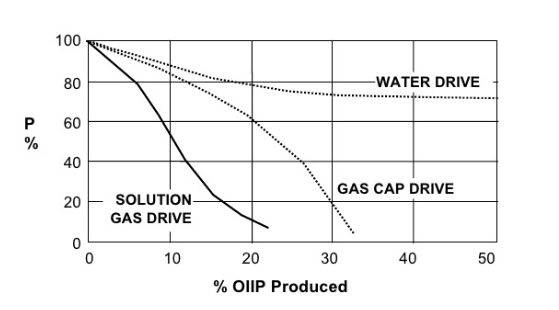
\includegraphics[width=8cm, height=5cm]{figures/ReservoirPerformancePrimary.png}
       \end{center}
     \caption{Pressure trends under various drive mechanisms.}
  \label{fig:ReservoirPerformancePrimary}
\end{figure}

\item[\textbf{Gas cap drive}] 
As production continues, the gas cap expands pushing the gas-oil 
contact (GOC) downwards. Eventually the GOC will reach the production wells and 
the gas oil ratio (GOR) will increase by large amounts. The recovery of gas cap 
reservoirs can be (20\% to 40\% OOIP). 
%Produced gas can be separated and immediately injected back into gas cap.
\item[\textbf{Water drive}]
The drive energy is provided by an aquifer that interfaces with the oil in the reservoir at the 
oil-water contact (OWC). The recovery from water driven reservoirs is usually good (20-60\% OOIP). 
%As production continues, and oil is extracted from the reservoir, the aquifer expands into the reservoir displacing the oil. 
%Oil production from a strongly water driven reservoir remains fairly constant until 
%water breakthrough occurs. When water breakthrough does occur the well can 
%either be shut-down, or assisted using gas lift.
\item[\textbf{Gravity drainage}]
Gravity drainage is the fourth drive force that might be 
considered for drive mechanism where the density differences between oil and gas 
and water result in their natural segregation in the reservoir. This process is relatively weak and in practice is only 
used in combination with other drive mechanisms. 
%\subsection*{Combination drive}
%In practice a reservoir usually incorporates at least two 
%main drive mechanisms. Therefore, Combination or Mixed Drive can be accounted as 
%the fifth type of Drives \citep{Glover}. Oil lifting by gas or pumps: In 
%addition to the previous drive mechanisms, artificial lifting is considered as a 
%primary recovery, which is a process used to increase pressure within the 
%reservoir, when the natural drive energy of the reservoir is not strong enough 
%to push the oil to the surface. The two main categories of artificial lift 
%include pumping systems and gas lift. Gas lift method injects compressed gas 
%into the well to re-establish pressure, making it produce. On the other hand, 
%jack pumps are submersed and used to lift the oil to the surface \citep{Fleshman}.
\end{description}
\section{Secondary recovery}
After initial discover and production, typical oil reservoirs lose the drive 
mechanism of gas or water that originally forced the oil to the surface. The 
second stage of hydrocarbon production in which an external fluid such as water: 
usually named water flooding or water injection or gas: referred to as gas 
flooding or gas injection, is injected into the reservoir through injection 
wells. By secondary recovery methods, another 15-20\% may be produced.
\citep{Fleshman}.
\begin{description}[style=nextline]
\item[\textbf{Water flooding}]
Water Flooding is implemented by injecting water into a set of 
wells while producing from the surrounding wells. Water flooding projects are 
generally implemented to accomplish reservoir pressure maintenance and as a water drive to 
displace oil from the injector wells to the producer wells\citep{Fleshman}.
\item[\textbf{Gas flooding}]
This method is similar to water flooding in principal, and is used 
to maintain gas cap pressure even if oil displacement is not required. Usually 
the produced natural gas is re-injected to the reservoir in order to maintain 
reservoir pressure rather than to displace the hydrocarbon. 
\begin{figure}[ht]
\begin{center}
      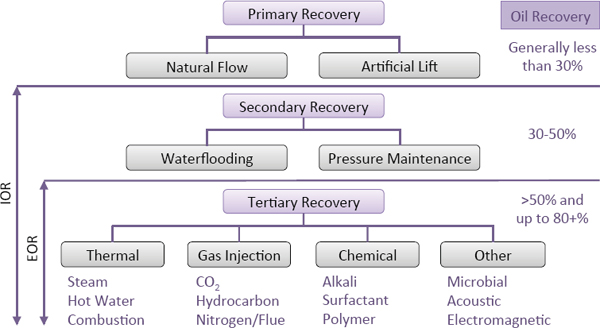
\includegraphics[width=10cm, height=6.5cm]{figures/OilRecoveryStages.png}
       \end{center}
     \caption{The different oil recovery stages and the corresponding oil recovery
factor.}
  \label{fig:OilRecoveryStages}
\end{figure}
%Traditional primary and secondary production methods typically recover one third 
%of oil in place, leaving two thirds behind. The reasons for this are not 
%difficult to understand. During the life of a well, there is always a point at 
%which the cost of producing an additional barrel of oil is higher than the price 
%the market will pay for that barrel. Production then halts. Under normal 
%circumstances, the well is abandoned, with 70\% of the oil left in the ground.
%Enhanced recovery techniques, EOR, can be used to recover additional 
%hydrocarbons. EOR introduces fluids that reduce viscosity and improve flow. 
%These fluids could consist of gases that are miscible with oil such as carbon 
%dioxide or nitrogen, steam, air or oxygen, polymer solutions, gels, 
%surfactant-polymer formulations, alkaline-surfactant-polymerformulations, or 
%microorganism formulations . However, the diagram of the oil recovery stages is 
%shown in Fig. 2 \citep{Lake_book89}.
\end{description}

\section{Enhanced oil recovery}
Enhanced oil recovery techniques refer to the recovery of oil through the injection of fluids and energy not 
normally present in the reservoir \citep{Romero}. The objectives of the 
injected fluids are to achieve mainly two purposes; First is to boost the 
natural energy in the reservoir; second is to interact with the reservoir 
rock/oil system to create conditions favourable for residual oil recovery that 
leads to reduce the interfacial tension between the displacing fluid and oil, 
increase the capillary number, reduce capillary forces, increase the drive water 
viscosity, provide mobility-control, create oil swelling, reduce oil viscosity, 
alter the wettability of reservoir rock \citep{Romero}. Enhanced oil 
recovery can be divided into two: thermal and non-thermal recovery \citep{Anazi}. Fig. 2 illustrates oil recovery stages by the different EOR 
techniques.
\subsection{Thermal techniques}
Thermal methods raise the temperature of the reservoir to heat the crude oil in 
the formation and therefore reduce its viscosity and/or vaporise part of the oil 
and thereby decrease the mobility ratio. The increase in heat reduces the 
surface tension, increases the permeability of the oil and improves the 
reservoir seepage conditions. The heated oil may also vaporise and then condense 
to be produced. This operation, however, requires substantial investment in 
special equipment. 
\begin{description}[style=nextline]
\item[\textbf{In-situ combustion (ISC)}]
In-situ combustion or fire flooding is a process in 
which an oxygen containing gas is injected into a reservoir where it reacts with 
the oil contained within the pore space to create a high temperature 
self-sustaining combustion front that is propagated through the reservoir. 
%The heat from the combustion thins out the oil around it, causes gas to vaporize 
%from it, and vaporizes the water in the reservoir to steam. Steam, hot water, 
%and gas, all act to drive oil in front of the fire to production wells. In-situ 
%combustion is possible if the crude-oil/rock combination produces enough fuel to 
%sustain the combustion front \citep{Romero}. Severe corrosion and 
%increased sand oil production are some of the problems that encountered by 
%implementation of this technique \citep{Romero}. 
\item[\textbf{Steam Injection}] 
Steam is injected into the reservoir either continuously or in 
cycles. %Continuous steam injection involves both injection and production wells, 
%whereas cyclic injection involves one well only which serves as both injection 
%and production well.
Steam floods are easier to control than in-situ combustion. 
For the same pattern size, the response time is 25-50\% lower than the response 
time for additional production by in-situ combustion \citep{Jelmert}.
\item[\textbf{Hot water flooding}]
Water-flooding in heavy oils is generally not an efficient 
way of production due to high viscosity of heavy oil compared to water. In hot 
water-flooding, thermal energy will increase oil mobility, and possibly improve
sweep efficiency \citep{Kermen}. 
%Injecting, regularly hot fresh to saline brines will improve oil recovery by dropping viscosity and decreasing 
%residual oil saturation. If low salinity waters are injected, clay matrix may 
%swell and therefore clog pore throats. Porosity and permeability can be 
%increased by collapsing some of the interlayer clays, when injecting water with 
%high temperature. According to \citep{Seni}, Burger and 
%others (1985) emphasized that although the incremental gain in production from 
%injecting hot water is substantial compared with that gained from injecting cold 
%water during typical water flood are less significant than those resulting from 
%injecting steam. Operators seldom employ hot water flooding because heat losses 
%in surface lines, wellbore, and formation are greater than the heat losses in 
%the other thermal processes. The heat losses reduce the processes effectiveness 
%in decreasing oil viscosity \citep{Ela}.
\end{description}
\subsection{Non thermal techniques}
\begin{description}[style=nextline]
\item[\textbf{Chemical Flooding}]
These processes use chemicals added to water in the injected fluid of a water 
flood to alter the flood efficiency in such a way as to improve oil recovery by: 
(i) Increasing water viscosity (polymer floods) (ii) Decreasing the relative 
permeability to water (cross-linked polymer floods) (iii) Increasing the 
relative permeability to oil (micellar and alkaline floods)  \citep{Glover} 
\item[\textbf{Polymer flooding}]
Polymers improve both vertical and areal sweep efficiency by 
reducing water-oil ratio. Polymers are injected through water injection wells in 
order to displace the residual oil. Increasing the displacing fluids viscosity 
and lowering its relative permeability through plugging \citep{Anazi}. 
\item[\textbf{Micelalr polymer flooding}]
It is well known that water and oil cannot be mixed 
until the third component, surfactant or soap, is added to reduce the 
interfacial tension between oil and water. Since micellar solution makes fluids 
miscible in the reservoir, almost 100\% of oil can be displaced especially in the 
presence of alkaline. However, due to reservoir rock non-uniformity in the field, the amount of oil recovered is reduced. 
 %The main objective of micellar injection is to reduce interfacial tension to enhance oil 
%recovery \citep{Zare}. 
%Micellar solutions are mixtures of surfactants, 
%co-surfactants, electrolytes, hydrocarbon, and water. Surfactants are substances 
%known as surface active agents, such as soap. Co-surfactants are used for 
%stability such as alcohols. Electrolytes are salts used to control viscosity and 
%interfacial tension such as sodium chloride or ammonium sulphate. \citep{Anazi}.
\item[\textbf{Alkaline-surfactant-polymer (ASP) flooding}]
During waterflooding residual oil is 
trapped due to low water viscosity and high water-oil interfacial tension, 
therefore another way is to inject the three chemicals; alkaline to minimize 
surface adsorption; surfactant to lower interfacial tension and stabilizes the 
emulsion. On the other hand, polymer is used to increase viscosity and to 
improve mobility control and sweep efficiency\citep{Kirk}. 
\end{description}
\subsection{ Nitrogen Injection}
%The nitrogen injection can be used in deep light to medium oil reservoirs mainly 
%containing \ce{C1} to \ce{C7} components. It is applicable in both the Sandstone and 
%Carbonate reservoirs.
Nitrogen itself is an inert gas that gets miscible at very 
high pressure and efficiently reduces the oil viscosity while providing efficient 
miscible displacement \citep{Syed}. Nitrogen can be used for the following
enhanced oil recovery applications: 
\begin{description}[style=nextline]
 \item [\textbf{Nitrogen immiscible flooding}]
%Gas cap displacement:The reservoir is a large anticlinal structure with a 
%sizable gas cap. 
Gas is being injected into the crest of the structure to 
maintain the pressure, to recover the hydrocarbon liquids in the gas cap, and to 
stabilize the gas/oil contact.
\item[\textbf{Nitrogen miscibility displacement mechanism}]
There are three types of miscibility including; First contact miscibility; Multi- contact miscibility; 
Vaporizing mass-transfer miscibility \citep{Shine}. 
\item[\textbf{Multi-contact miscibility}]
%In miscible flood processes some combination of transfer of components from the oil
%displaced to the injected fluid and from the injected fluid to the oil takes place as the phases flow through the porous 
%medium. Some hydrocarbon gases, with a high proportion of intermediate molecular 
%weight components (\ce{C3}, \ce{C4}, and\ce{C5}) are miscible with oil under pressure and 
%temperature conditions encountered in some oil reservoirs. Moreover, under much 
%wider condition the displacement of oil by hydrocarbon gases may lead, through 
%component exchange between oil and the gas, to creation of transition zone in 
%which the composition varies continuously between the composition of the 
%displacing fluid and the composition of the oil. Light to intermediate 
%components are exchanged between oil and injected fluid. A transition zone 
%spreads out in which both fluids are miscible. 
This type of miscibility is  subdivided into vaporizing gas drive, 
condensing gas drive\citep{Juttner}.

%\subsubsection*{Vaporising gas drive}
%It is a particular case of multiple contact 
%miscibility, based on the vaporization of intermediate components from the 
%reservoir oil to the injected gas creating a miscible transition zone. The \ce{\ce{C2}}-\ce{C5} 
%fraction is preferently extracted. This mainly occurs at high pressure, by 
%injecting natural (hydrocarbon) gas, flue gas or nitrogen. When Nitrogen is 
%injected at high pressure, it can form a miscible slug which aids in freeing the 
%oil from the reservoir rock.
%\subsubsection*{Gravity drainage}
%Gravity enhancement is by using the gravity drainage potential 
%of a dipping or thick hydrocarbon zone. (Nitrogen, which usually has a lower 
%density than the reservoir fluids, when injected into the crest or allowed to 
%migrate to the crest, will enhance the down dip displacement and production of 
%the reservoir fluids or of a gravity stable miscible slug) \citep{Clancy}.
%One of the most common gravity drainage processes is the Double 
%Displacement Process (DDP). This is done by injecting gas up -dip and producing 
%oil down-dip \citep{Shine}. By using Gravity Drainage, piston like 
%displacement is obtained, therefore gas fingering is avoided. In addition, the 
%following results are obtained: Horizontal gas-oil contact; gravity dominate the 
%gas flow; optimized time between gas injection and oil production as fast as 
%possible; the greater the dip angle the higher the injection and production 
%rates w/o gas fingering; the greater the dip the more effective the gravity 
%drainage \citep{Walker}.
\item[\textbf{Gas Flooding Injection}]
Gas is generally injected single or intermittently with water and this manner of 
injection called Water-Alternating-Gas (WAG), has become widely practiced over 
all of worlds oil fields \citep{Kulkarni}. According to miscibility 
between gas injected and oil displaced, gas injection can be classified into two 
major types: miscible gas injection and immiscible gas injection.
In miscible gas injection, the gas is injected at or above minimum miscibility 
pressure (MMP) which causes the gas to be miscible in the oil.
In contrast in immiscible gas injection, flooding by the gas is conducted below MMP. This low 
pressure injection of gas is used to maintain reservoir pressure to prevent 
production cut-off and thereby increase the rate of production \citep{Anazi}. 
In miscible flooding, the incremental oil recovery is obtained by one 
of the three mechanisms: oil displacement by solvent through the generation of 
miscibility (i.e. zero interfacial tension between oil and solvent hence 
infinite capillary number), oil swelling, and reduction in oil viscosity 
\citep{Kulkarni}. Miscible fluids are 100\% soluble in each other. The 
interfacial tension between miscible fluids is zero. Injection gases include:
\item[\textbf{LPG injection}]
Miscible LPG products such as ethane, propane, or butane have 
first contact miscibility, which means they will be miscible from the first 
contact with oil. However, LPGs are in such demand as marketable commodity that 
their use in EOR is limited \citep{Romero}. In particular, this process 
uses a slug of propane or other liquified petroleum gas (2 to 5\% of pore volume 
PV) followed by natural gas, inert gas, and/or water. Thus, the solvent will 
bank oil and water ahead, and fully displace all contacted oil \citep{Anazi}.
\item[\textbf{Enriched gas miscible process}]
In this process, a slug of methane (\ce{C1}) enriched 
with ethane (\ce{C2}), propane (\ce{C3}), or butane (\ce{C4}) (10\% to 20\% of the PV) and 
followed by lean gas and/or water is injected from water injection well into the 
reservoir. When the injected gas contacts virgin reservoir oil, \ce{C1}-\ce{C3} are 
quenched from the injected gas and absorbed into the oil \citep{Anazi}. 
The injected HC solvent is usually displaced with cheaper chase leaner or inert 
gas like Methane or Nitrogen. At reservoir conditions the most usual problem 
occurs with the hydrocarbon miscible flood is the gravity over-ride because of 
its lighter density than the oil and water. So that in any miscible flood the 
Minimum Miscibility Pressure (MMP) plays the most major role to overcome this 
problem. As a remedial factor the solvent is to be injected at or above the MMP 
of the reservoir fluid. Once it becomes miscible then it improves the sweep 
efficiency and fallouts in optimum recovery \citep{Syed}.
\item[\textbf{Carbon dioxide (\ce{CO2} ) injection}]
Is one of the most proven of these methods. Almost pure \ce{CO2} 
(>95\% of the overall composition) has the property of mixing with the oil to 
swell it, make it lighter, detach it from the rock surfaces, and causing the oil 
to flow more freely within the reservoir so that it can be swept up in the 
flow from injector well to producer well \citep{Melzer}. Flooding a 
reservoir with \ce{CO2} can occur either miscibility or immiscibly. Miscible \ce{CO2} 
displacement is only achieved under a specific combination of conditions, which 
are set by four variables: reservoir temperature, reservoir pressure, injected 
gas composition, and oil chemical composition. From a fundamental point of view, 
\ce{CO2} EOR works on a very simple principle, namely, that given the right physical 
conditions, \ce{CO2} will mix miscibly with oil, acting much like a thinning agent, 
the same way that gasoline does with motor oil. After miscible mixing, the fluid 
is displaced by a chase phase, typically water \citep{Meyer}. 
In this thesis \ce{CO2} injection as EOR method is going to by examined.
\end{description}
\section {Need for simulation and optimization}
Use of reservoir simulation has grown because of its ability to predict the 
future performance of oil and gas reservoirs over a wide range of operating 
conditions. Reservoir simulators use numerical methods and high-speed computers 
to model multidimensional fluid flow in reservoir rock. Technology improvements have enabled 
a widespread use of integrated simulation models for a better asset management 
to be fully combined with measured field data. Reliable simulators and 
adequate computing capacity are available to most reservoir engineers, so 
simulation is usually practical for all reservoir sizes and all types of 
reservoir performance studies. Although the use of simulation frequently is 
optional, it may be the only reliable way to predict the performance of a large, 
complex reservoir, especially if such external considerations as government 
regulations influence the production schedule. Even for small reservoirs where 
simple calculations or extrapolations may be adequate, simulation is often 
faster, cheaper, and more reliable than alternative methods for predicting 
performance.\citep{Mattax}

In petroleum fields, hydrocarbon production is often constrained by reservoir 
conditions, deliverability of the pipeline network, fluid handling capacity of 
surface facilities, safety and economic considerations, or a combination of 
these considerations. Optimization of reservoir development requires many 
evaluations of the possible combinations of the decision variables in order to 
obtain the best economical strategies. The objective of dynamic production 
optimization is to find the best operational settings at a given time, subject 
to all constraints, this gives you greater production gains for longer. 
Overall, optimization delivers a faster return on investment during initial 
production, yields greater revenues during plateau and decline, and delays well abandonment.
Given the fact that oil prices continue to drop to their lowest levels in 
several years, oil industry will inevitably turn to optimization in order to continue to 
deliver the dividend levels that investors have come to expect. Production 
optimization is no longer an option it is a necessity.

\section{Previous work}
In petroleum industry, optimization methods are necessary for history 
matching, where we adjust the physical properties of the 
reservoir model, and for optimization of production, where the objective is to maximize either the net present value 
or the cummulative production of hydrocarbons.
All the above methods can be 
implemented both with gradient-free and gradient-based techniques. 
Generally, gradient-free techniques are not necessarily guaranteed to find the true global optimal solution, they converge 
very slowly and require high performance computing infrastructures.
On the other hand, for gradient-based techniques, once the gradient is computed there are several options for finding an optimum.
Furthermore, proper exploitation of gradient information can significantly enhance the speed of convergence in comparison with a method
that does not compute gradients. Another feature of gradient-based methods is that they provide a clear convergence criterion.

Among gradient-based algorithms we consider only the adjoint approach for compositional reservoir
simulation problems.Procedures of this type entail the application of optimal
control theory and have their roots in the calculus of variations
\citep{Bryson:1975,Stengel:1986}. Adjoint-based optimization techniques have 
been used in a reservoir simulation setting both for history matching (see, e.g.,
\citep{Gavalas,Chavent,Li,Oliver,Pallav:2006}) and for production 
optimization. Much of the early work on their use for optimization of oil recovery was 
performed by Ramirez and coworkers, who considered the optimization of several different
enhanced oil recovery (EOR) processes \citep{Ramirez:book,Ramirez:1989,Ramirez:1993}. In subsequent work, the focus 
was on gradient-based optimization (and in some cases on the optimization of `smart
 wells') for water flooding \citep{Asheim,Virnovski,Sudaryanto:2000,Brouwer:2004,Pallav:2006}. 
 %Recent 
%studies have addressed the implementation of adjoint-based procedures into general
%purpose simulators, the treatment of general constraints, and regularization and
%other numerical issues \citep{Pallav:2008,Brouwer:2008,Doublet:2009,CPRA}.
Refer to \citep{Jansen:2011} for a more complete overview of adjoint-based 
optimization methods. We note additionally that, although not considered here, 
derivative-free methods can also be applied for production optimization problems -- see
\citep{echeverria:2011} for discussion and examples.
% Although much of the early (1980s) work noted above focused on the application
% of adjoint procedures for EOR problems, there has not been much work on the use
% of adjoint techniques for large-scale (practical) compositional reservoir
% simulation problems.This is likely due to the complexity entailed in
% implementing adjoint procedures into a general purpose compositional reservoir
% simulator and to the challenging computational problems that must be solved to
% perform the optimizations. 
Recently an adjoint treatment for multicomponent oil-gas
compositional systems was presented in~\citep{Kourounis2014}. 
The formulation included an extensive discussion on engineering
constraints that should usually be taken into account in realistic scenarios. 
These constraints appear either as bounds (box constraints) 
on the control variables or as inequality constraints on 
nonlinear functions of the controls and states of the underlying PDEs.
 Two treatments were proposed for the nondifferentiable constraints: a formal 
treatment within the optimizer performing lumping for all wells and time steps, and a heuristic 
approach, where bound constraints are treated in the optimization and nondifferentiable 
constraints are satisfied in the forward model. The investigation showed that 
although standard lumping techniques perform well for simple academic problems, they fail 
to obtain optimal solutions better than the reference for realistic problems.
That result motivated further developments of formal constraint-handling 
techniques. In ~\citep{Kourounis2015} the author introduces a new formal treatment for the 
nondifferentiable  constraints where lumping is avoided to allow for a more realistic 
discretization of the nonlinear constraints. The performance of the new approach is compared to
the ones introduced in~\citep{Kourounis2014} for several different examples
of increased complexity. 

\section{The scope of this work}
Optimization using gradients converges much faster than gradient-free techniques 
resulting in significant saving in computational time but it usually gets 
trapped to poor local optima~\citep{Kourounis2014,Kourounis2015}. 

The aim of this work is to exploit an observation in homogeneous reservoirs, 
where the global optimum, when optimising cumulative oil recovery,  is usually 
achieved from any initial guess. We perform continuation with 
respect to a parameter that transforms the homogenous reservoir with respect to 
porosity and permeability, gradually to the original inhomogeneous one, solving an optimal 
control 
problem for each distinct value of the parameter. This approach allows us to follow the optimal solution
(cummulative recovery or ...?residual oil?...) as the geology switches from homogeneous to inhomogenous.
This novel technique is presented at the best of our knowledge for first time for 
production optimization problems and tested in several examples of increased complexity.



 







\endinput
%%% Local Variables: 
%%% mode: latex
%%% TeX-master: "ptyxiakn"
%%% End: 




%%%%%%%%%%%%%%%%%%%%%%%%%% Part two %%%%%%%%%%%%%%%%
\part{Theory on production optimization and methods}
%%%%%%%%%%%%%%%%%%%%%%%%%%%%%%%%%%%%%%%%%%%%%%%%%%%%


%%%%%%%%%%%%%%%%%%%%%%%%%%%%%%%%%%%%%%%%%%%%%%%%%%
\chapter{Production Optimization}
%%%%%%%%%%%%%%%%%%%%%%%%%%%%%%%%%%%%%%%%%%%%%%%%%%
The optimization of oil production is a tedious and computational intensive 
process that requires the solution of time dependent nonlinear set of partial 
differential equations describing the flow of hydrocarbons in anisotropic porous 
media. The optimization of time-varying well settings, such as injection rates, 
production rates or bottom-hole pressures, is an important aspect of optimal 
reservoir management. Optimization of production is usually performed using either gradient 
free techniques like genetic, particle swarm algorithms, or gradient-based 
techniques where the gradients are computed through the solution of the adjoint 
problem.

\section{Gradient-free methods}
In this section we review the basic gradient-free method
employed in industry and academia for the solution of several
optimal control problems of the oil industry.
\subsection{Genetic algorithms (GAS)}
Genetic algorithms are commonly used to generate high-quality solutions to 
optimization and search problems by relying on bio-inspired operators such as 
mutation, crossover and selection.The method is a general one, capable of being 
applied to an extremely wide range 
of problems.
Genetic algorithms are based on three essential components:

- Survival of the fittest (Selection).

- Reproduction processes where genetic traits are propagated (Crossover).

- Variation (Mutation).
\subsection{Particle Swarm Optimization(PSO)}
Particle swarm optimization (PSO) is  is a stochastic, population-based computer algorithm.
It applies the concept of swarm intelligence (SI) to problem solving.
Swarm intelligence is the property of a system whereby the collective behaviors of 
(unsophisticated) agents interacting locally with their environment cause 
coherent functional global patterns to emerge (e.g. self-organization, emergent 
behavior). Gradient-free methods are not necessarily guaranteed to find the true global 
optimal solutions, but they are able to find many good solutions.

\section{Gradient-based methods}
Gradient-based optimization methods offer the advantage to construct additional 
information about the shape of the surface for the particular problem. Hence, 
the gradient of a function provides information about the behavior of a 
function such as steepness and extrema in the parameter space. The gradients are 
computed through the solution of the adjoint problem.  With this additional 
information, the convergence of the search algorithm can be drastically 
enhanced.
\subsection{Sequential quadratic programming (SQP) }
Sequential quadratic programming (SQP) is an iterative procedure that utilizes a 2.order approximation of
the Lagrangian function of a problem. The quadratic formulation of the problem is a local approximation
of the real problem and consists of a quadratic objective function and linear equality
and/or inequality constraints. SQP can be used both within a trust-region and a line
search framework. In a line search framework, the algorithm proceeds by first calculating
a search direction. If we are trying to maximize the original problem, a function is then
solved that maximize the quadratic approximation in the search direction. When a
new iteration point in the direction that was searched has been reached, a new local
approximation is constructed and the algorithm proceeds to the next iteration given that
a set of optimality conditions has not been fulfilled.
SQP is a generalization of Newtons method for unconstrained problems as it uses a
quadratic approximation of the Lagrangian function, steps in a direction it believes the
optimum lies, and then creates a new approximation of the original model when a new
iteration point has been reached. The main difference between Newtons method and
SQP is that for constrained nonlinear problems the Taylor approximation of the original
problem cannot be used, as the model problem also needs to incorporate the constraints
of the original problem. Instead, the Lagrangian function is used and the constraints of
the problem thereby taken into account. SQP is appropriate for small and large problems and it 
is well-suited to solving problems with significant nonlinearities\citep{Bonnans}.
\subsection{Interior point optimization (IPO)}
An interior point method is a linear or nonlinear programming method that 
achieves optimization by going through the middle of the solid defined by the 
problem rather than around its surface. This method is further discussed in section....


Both gradient-based and derivative-free methods have been considered for this 
problem, and both are applicable in different situations. 
A gradient-based optimization method, in which the gradient is computed using 
an adjoint formulation, is often the method of choice since in contrast to 
numerical perturbation techniques that require as many objective function 
evaluations as the number of control parameters, the gradient using 
adjoint-based techniques is obtained  only at a small fraction of the time 
spent for the evaluation of the objective function.  The development of adjoint 
procedures for general compositional flow problems is 
much more challenging than black-oil simulation because of the need to perform
phase-equilibrium (flash) calculations for all grid blocks at every iteration 
of every time step. Adjoint formulations are challenging to code
because they require analytical derivatives of many variables, and the
increased complexity of compositional simulators renders these derivatives
much more cumbersome to calculate than in the case of a black-oil simulator.
Furthermore, the production optimisation problem is usually subject to industrial 
constraints, for example, maximum gas rate specification in injection or 
production wells, when the control variables are well bottom-hole pressures. At 
the same time optimising  time-varying well settings, such as injection rates, 
production rates or bottom-hole pressures, is an important aspect of optimal 
reservoir management that increases significantly the dimension of the search 
space. It is well known that for non-convex optimisation problems, 
gradient-based techniques are likely get trapped in poor local optima. A common 
practise is to lunch several independent optimisation from different initial 
guesses or to combine ideas from gradient-free algorithms with gradient-based 
to benefits from the merits of both. An adequate sampling of the search space 
would require an intractable number of simulations and it is thus impossible.



%%%%%%%%%%%%%%%%%%%%%%%%%%%%%%%%%%%%%%%%%%%%%


\section{Oil-gas compositional simulation equations} \label{sec:forward}


The mass conservation equation for component $i$, which can exist in any
phase $j$ (here $j=o,~g$, where $o$ indicates oil and $g$ gas), is given
by \cite{Cao:Thesis,Voskov_nonlinear:2009,Voskov:2012}:
%
\begin{align}
\label{transport_eq_ci}
\dfrac{\partial}{\partial t} \left(\phi
  \sum_{j} x_{ij} \rho_j S_j \right)
    - \nabla \cdot \left ( \sum_{j} x_{ij} \rho_j  \boldsymbol{\tens{K}}
      \dfrac{k_{rj}}{\mu_j}\nabla \Phi_j \right ) + \\ \sum_{w} \sum_{j} x_{ij} \rho_j q_j^w = 0, \ \ i = 1,\ldots,n_c. \nonumber
\end{align}
%

In the first (accumulation) term, $t$ is time, $\phi$ is porosity, $x_{ij}$
designates the mole fraction of component $i$ in phase $j$, $S_j$ is saturation,
and $\rho_j$ is molar density. In the second (flow) term,  $\boldsymbol{\tens{K}}$ 
is the permeability tensor, $k_{rj}$ is the relative permeability to
phase $j$, $\mu_j$ the phase viscosity, and the phase potential
$\Phi_j$ is given by $\Phi_j = p_j-\rho_j g(D-D^0)$, where $p_j$ is
phase pressure, $D$ is depth, $D^0$ is a reference depth, and $g$ is
gravitational acceleration. In the third (source/sink) term, $q_j^w$
indicates the phase flow rate for well $w$. The treatment of this term will be discussed in Section~\ref{sec:constr-sim}. Equation~(\ref{transport_eq_ci}) is written for each of the $n_c$
components present in the system.

For a mixture of $n_c$ components in two fluid phases (oil and gas), thermodynamic equilibrium
can be expressed as:
%
\begin{equation} \label{general_therm_system1} f_{io}(p_o, x_{io}) - f_{ig}(p_g,
  x_{ig}) = 0,  \end{equation}
%
where $f_{io}(p_o, x_{io})$ is the fugacity of component $i$ in the oil phase and $f_{ig}(p_g, x_{ig})$ 
is the fugacity of component $i$ in the gas phase (temperature does not appear because the system is assumed to
be isothermal).
%and $n_p$ is the number of phases (here $n_p=2$).
We additionally must satisfy the saturation constraint ($S_o+S_g=1$) and the
component mole fraction constraints:
%
\begin{align}\label{eqn:MoleFractionCons} \sum_{i=1}^{n_c} x_{i0} -1 = 0, \ \ \
    \ \ \ \ \sum_{i=1}^{n_c} x_{ig} -1 = 0.  \end{align}
%
A capillary pressure relationship also appears in cases with nonzero capillary
pressure, though here we neglect capillary pressure so $p_o=p_g$.

As discussed by many authors (see, e.g.,
\cite{Coats:1980,Cao:Thesis,Voskov:2012,Young:1983}), the system described
above contains a total of only $n_c$ primary equations and primary variables per
grid block. These equations and variables are coupled (from block to block), and
in a fully-implicit method are all computed simultaneously at each Newton
iteration. The remaining (secondary) variables can be computed locally (block by
block), and thus very efficiently, once the primary variables are determined.
Various options exist for the choice of primary variables (see
\cite{Voskov:2012} for discussion). Here we use the so-called natural variable
set, which includes, for each grid block, one pressure unknown, $n_p-1$
saturation unknowns (where $n_p$ is the number of phases; here $n_p=2$), and $n_c-n_p$ component mole fraction unknowns.

In our formulation, the governing equations (\ref{transport_eq_ci}) are solved
fully-implicitly, using a backward-Euler time discretization, two-point flux
approximation, and single-point upwinding \cite{Aziz_book79}. These treatments
are standard in practical reservoir simulation. For the solution of the set of
nonlinear equations, we use Newton's method with the solution at the previous
time step as the initial guess. A limit on the change of the grid-block
saturation and mole fractions over a Newton iteration is applied
\cite{Younis:2010}. The Newton iterations terminate when the maximum relative
norm of the residual is less than $10^{-6}$ (tight convergence criteria are required for the adjoint solution, discussed below). For the solution of the
linear system at each Newton iteration we use GMRES preconditioned by the
constrained pressure residual method, as described in~\cite{CPRA}. Iteration is
terminated when the Euclidean norm of the initial residual has decreased by five
orders of magnitude.

We employ a simple time stepping strategy. The time step size at step $n+1$ is a
multiple of that at $n$, provided nonlinear convergence was achieved at step
$n$. In this way the time step can increase until it reaches the maximum
allowable value. If the nonlinear solver fails to converge within a prescribed number
of Newton iterations, we divide the time step by a fixed constant. This process
is repeated until the nonlinear system converges.



\section{Adjoint equations for the compositional system} \label{sec:adjoint}
We now present the discrete and continuous adjoint equations. Some numerical and coding issues are also discussed.


\subsection{Automatic differentiation} \label{sec:autodiff}


It is quite common for comprehensive computational platforms, in reservoir
simulation and other application areas, to undergo frequent modification and enhancement. This poses a problem for adjoint formulations
because, when an existing feature is modified the corresponding adjoint code may
also be impacted, and when a new feature is added, the associated adjoint code
must (in many cases) be written. The maintenance and development of adjoint code
poses challenges because the necessary derivatives are generally complicated.
This is particularly the case in compositional simulation where variables couple
in many ways, including through the nonlinear equation of state.


Automatic differentiation, or AD, is gaining popularity in the field of
scientific computing as a means of facilitating the development and enhancement of large code bases. AD enables, for example, the fast (analytical) determination of Jacobian matrix elements from the code
defining the residual vector. The use of AD has allowed the fast construction
and assessment of different compositional formulations within the same code
\cite{Voskov_nonlinear:2009}. In this work, we take advantage of AD to automate
the construction of many of the derivatives required for the adjoint
formulation.


The AD implementation used in our compositional simulator is the `automatic
differentiation expression templates library' (ADETL), developed originally by
Younis and Aziz~\cite{Younis:2007}.  This library generates efficient computer
code for the evaluation of the Jacobian matrix and the corresponding partial
derivatives from discrete algebraic expressions of the governing conservation
equations, associated constraint relations, and equations of state. We refer to
\cite{Younis:2007} for a detailed description of the underlying theory.


\subsection{Discrete adjoint formulation} \label{section:discreteAdjoint}

Following the fully-implicit discretization of the governing equations (using the usual finite volume method, with treatments as noted above), we can express the nonlinear system as:
%
\begin{align}
\label{eq:DiscretizedEquations}
\p_n(\x_n, \x_{n-1}, \u_n) =  \0 \rm,
\end{align}
%
where $\p_n$ denotes the fully discretized, both in space and time,
set of partial differential equations. Here $\x_n = \x(t_n)$ and $\u_n =
\u(t_n)$ are the states and controls (well settings), respectively, at time step $n$. The corresponding time step size
is designated $\Delta t_n$. We will use throughout the notation $\partial \p^T / \partial \x$ to denote the matrix $(\partial \p / \partial \x)^T$.



We are interested in either maximizing or minimizing
an objective function $\myobj$ that is in general a nonlinear function of the
states $\x_n$ and the controls $\u_n$ of the forward problem. We
assume that $\myobj$ has the following form:
%
\begin{align}
  \label{eq:continuousObjective}
  \myobj(\x, \u) = \integral{\F\left ( \x(t), \u(t) \right )} + \M(\x(t_N)),
\end{align}
%
where $\F(\x(t), \u(t))$ is a nonlinear function varying with time and $\M(\x(t_N))$ is a
function of only the last state $\x_N$. After the solution of the
forward problem has been obtained, $\myobj$ may be approximated by
%
\begin{align}
  \label{eq:discretizedObjective}
  \myobj \approx \fsum{n=1}{N}{ \Delta t_n \, \F_n \left ( \x_n, \u_n \right ) + \M(\x_N) }.
\end{align}
%

Using (\ref{eq:discretizedObjective}) we can state the optimal control
problem as:
%\\
%\begin{tabular}{ll}
%Extremize  &
%  $\displaystyle f =
%  \fsum{n=1}{N}{ \Delta t_n \, \F_n \left ( \x_n, \u_n \right ) + \M(\x_N) }$ \\
%  subject to &
%$\p_n(\x_n, \x_{n-1}, \u_n) = \0$, \\
%and &
%$\x_0 = \x(t_0)$.
%\end{tabular}
%\\ \\
\[
   \newproblem{NLP}{\u}{\displaystyle \myobj =
  \sum_{n=1}^N \Delta t_n \, \F_n \left ( \x_n, \u_n \right ) + \M(\x_N) }
                 {\p_n(\x_n, \x_{n-1}, \u_n) = \0,}
                 {\x_0 = \x(t_0)}.
\]

In general, a number of linear and nonlinear constraints may need to be included in the optimal
control problem. We postpone the discussion of their treatment until Section~\ref{sec:constraints}. 
Now, since $\p_n = \0$, we can introduce the augmented objective function $\myobj_A$ by `adjoining' 
the governing equations to the original objective function $\myobj$. The new objective $\myobj_A$ shares
the same extrema as $\myobj$ and is defined as:
%
\begin{align}
\label{eq:JAdefinition}
  \myobj_A = \fsum{n=1}{N}{\left ( \Delta t_n \F_n(\x_n, \u_n)
      + \blambda^T_n \p_n (\x_n, \x_{n-1}, \u_n)  \right )}
   + \M(\x_N).
\end{align}
%
In (\ref{eq:JAdefinition}), the vectors $\blambda_n$ are the Lagrange multipliers.


The maximum or minimum of $\myobj_A$ (and thus $\myobj$) is achieved when the first variation of $\myobj_A$ is 
zero ($\delta \myobj_A=0$). After performing some index-shifting, and grouping
terms multiplied by the same variation ($\delta \x_n, \delta \x_N,
\delta \u_n$), $\delta \myobj_A$ can be written as:
%
\begin{align}
\label{eq:discreteAfterRegrouping}
  \delta \myobj_A &=
  \left (
    \pder{\M_N}{\x_N}
    + \Delta t_N \pder{\F_N}{\x_N}
    + \blambda_N^T\pder{\p_N}{\x_N}
    \right ) \delta \x_N
    \nonumber \\
    &+\fsum{n=1}{N-1}{
      \left (
        \Delta t_n \pder{ \F_n}{\x_n}
        +\blambda^T_{n+1}\pder{\p_{n+1}}{\x_n}
        +\blambda^T_n\pder{\p_n}{\x_n}
      \right ) \, \delta \x_n
    } \nonumber \\
    &+\fsum{n=1}{N}{
      \left (
        \Delta t_n \pder{\F_n}{\u_n}
        +\blambda^T_n\pder{\p_n}{\u_n}
      \right ) \, \delta \u_n.
    }
\end{align}
%
In order to achieve $\delta \myobj_A=0$, we require $\delta \myobj_A / \delta \x_n=\0^T$ (for $n=1,2, \ldots, N$) and $\delta \myobj_A / \delta \u_n=\0^T$. To satisfy $\delta \myobj_A / \delta \x_n =\0^T$ for $n=1,2, \ldots, N$, we require that the Lagrange multipliers satisfy the following equations:
%
\begin{align}
\label{eq:discreteODE}
 \pder{\p_n^T}{\x_n}  \blambda_n &= -
 \left (\pder{\p_{n+1}^T}{\x_n} \blambda_{n+1} + \Delta t_n \pder{\F^T_n}{\x_n}
 \right ),% \quad n=1,2,\ldots,N-1
\\
\label{eq:discreteBC}
  \pder{\p_N^T}{\x_N} \blambda_N &= -
  \left ( \Delta t_N \pder{\F^T_N}{\x_N} + \pder{\M_N^T}{\x_N} \right ).
\end{align}
%
With this choice of the Lagrange multipliers the total variation becomes
\begin{align*}
  \delta \myobj_A =
    \fsum{n=1}{N}{
      \left (
        \Delta t_n \pder{\F_n}{\u_n}
      +\blambda^T_n\pder{\p_n}{\u_n}
      \right ) \, \delta \u_n ,
    }
\end{align*}
and the gradient of the objective function with respect to the controls is
\begin{align}
\label{eq:optimizerDiscreteGradient}
  \frac{\delta \myobj_A}{\delta \u} = \left [
  \frac{\delta f_1}{\delta \u_1}, \frac{\delta f_2}{\delta \u_2},
  \ldots,
  \frac{\delta f_N}{\delta \u_N} \right ].
\end{align}
The individual entries of $\delta \myobj_A/\delta \u$ are given by
%\footnote{If possible give some proof of this derivation}
\begin{align}
\label{eq:discreteGradient}
  \frac{\delta f_n}{\delta \u_n} =
  \Delta t_n  \pder{\F_n}{\u_n}
  +\blambda^T_n\pder{\p_n}{\u_n}, \quad n=1,2,\ldots,N.
\end{align}
%
By driving $\delta \myobj_A / \delta \u$ to zero, we achieve the minimum or 
maximum of $\myobj_A$ (and thus $\myobj$). In practice, $\delta \myobj_A / \delta \u$, 
along with other quantities related to constraints, are provided to a 
gradient-based optimization algorithm to determine the next estimate for the controls $\u$.

In optimization problems, the well control variables do not typically change at each time step in the flow simulation. Rather, they are defined over longer time periods that are referred to as control steps. Time steps are usually small in order to capture flow dynamics, reduce time-discretization error, and facilitate convergence of the Newton iterations. 
The gradient at the control period $m$, $\delta f_n/\delta \u_m$, is simply the sum of
the gradients $\delta f_n/\delta \u_n$ for all time steps that belong to control period $m$.


\subsection{Continuous adjoint formulation}
\label{section:continuousAdjoint}
The continuous adjoint formulation employs the continuous
representation of the objective function along with the spatially discretized reservoir flow equations. The optimal control problem can then be stated as:
%\\
%\begin{tabular}{ll}
%Extremize&
%  $\displaystyle f(\x, \u) = \integral{ \F(\x(t), \u(t)) } + \\M(\x(t_N))$
%\\
%subject to &
%$\p(\dot{\x}(t), \x(t), \u(t) ) = \0$.
%\end{tabular}
%\\ \\
\[
   \problem{}{\u}{\displaystyle \myobj(\x, \u) = \integral{ \F(\x(t), \u(t)) } + \M(\x(t_N))}
                 {\p(\dot\x(t), \x(t), \u(t) ) = \0.}
\]


In this case we express the governing set of partial differential
equations, for a specified dynamic well-control strategy $\u(t)$, as $\p(\dot{\x}(t), \x(t), \u(t) ) = \0$.  
We introduce the Lagrange multipliers $\blambda(t)$  and define the Lagrangian $\L$ as:
%
\begin{align}
  \label{eq:lagrangian}
  \L(\dot{\x}, \x, \u, \blambda) = \F(\x, \u) + \blambda^T \, \p(\dot{\x}, \x, \u ),
\end{align}
%
The
variables $\u(t)$, $\x(t)$, $\dot{\x}(t)$ and $\blambda(t)$ are denoted
as $\u$, $\x$, $\dot{\x}$ and $\blambda$ to simplify notation. The
augmented objective function, $\myobj_A$, can be expressed as:
%
\begin{align}
  \myobj_A(\dot{\x}, \x, \u, \blambda) = \integral{\L(\dot{\x}, \x, \u, \blambda)} + \M(\x_N).
\end{align}
%
The first variation of $\myobj_A$ is given by
%
\begin{align}
\label{eq:firstvariation}
  \delta \myobj_A
  &= \integral{
    \left (
    \pder{\L}{\dot{\x}} \, \delta \dot{\x}
  + \pder{\L}{\x} \, \delta \x
  + \pder{\L}{\u} \, \delta \u
  + \pder{\L}{\blambda} \, \delta \blambda \right ) }
  \nonumber \\
  &+ \pder{\M(\x_N)}{\x_N} \, \delta \x_N.
\end{align}
%
Note that $\delta \dot{\x} = d (\delta \x) / d t$, so any variation in
the state vector $\x$ will introduce a
variation in its time derivative $\dot{\x}$.

After integration by parts, using the fact that the variation of the initial conditions $\delta \x_0 = \0$, and
taking into account that $\partial \L^T / \partial \blambda = \p(\dot \x, \x, \u) \, = \0$,
the first variation of $\myobj_A$ can be written as:
%
\begin{align}
\label{eq:augmentedobjective}
  \delta \myobj_A
  &= \integral{
    \left(
      \pder{\L}{\x}  -\dder{}{t} \pder{\L}{\dot{\x} }
    \right) \, \delta \x} \nonumber \\
 &+ \left ( \pder{\L(\x_N)}{\dot{\x}_N} + \pder{\M(\x_N)}{\x_N} \right )
  \, \delta \x_N \nonumber \\
  &+ \integral{ \pder{\L}{\u} \, \delta \u }.
\end{align}
%
To achieve $\delta \myobj_A / \delta \x=\0$, $\blambda$ must be chosen
to satisfy the following:
%
\begin{align}
\label{eq:continuousadjointode}
  &\dder{}{t} \left ( \pder{ \p^T }{\dot \x} \blambda \right )
    - \pder{\p^T}{\x} \blambda - \pder{\F^T}{\x} = \0
\\
\label{eq:terminatingbc}
&\pder{\p^T_N}{\dot{\x}_N} \blambda_N = -\pder{\M^T(\x_N)}{\x_N}.
\end{align}
%
The ordinary differential equation in (\ref{eq:continuousadjointode}) is integrated backwards in
time starting from the final time condition
(\ref{eq:terminatingbc}). With the resulting $\blambda$, the first variation of the objective function becomes:
\begin{align}
  \delta \myobj_A = \integral{ \left ( \pder{\F}{\u} + \blambda^T
      \pder{\p}{\u} \right ) \, \delta \u}.
\end{align}


In order to allow a direct comparison of the discrete and continuous adjoint formulations,
we integrate the continuous adjoint backwards in time fully implicitly,
using the same scheme as is applied for the forward problem. The discrete
form of (\ref{eq:continuousadjointode}) is:
\begin{align}
  \label{eq:continuousODE}
  \pder{\p^T_n}{\x_n} \blambda_n
  = -  \pder{\p^T_{n+1}}{\x_n} \blambda_{n+1} -
   \Delta t_n \pder{\F^T_n}{\x_n}.
\end{align}
This equation is solved backwards in time, starting from the boundary condition~(\ref{eq:terminatingbc}).
Once the Lagrange multipliers have been obtained, the gradient is computed using
equations~(\ref{eq:optimizerDiscreteGradient}) and (\ref{eq:discreteGradient}). 
 

\subsection{Continuous versus discrete adjoint formulation}
The gradients obtained by the discrete adjoint formulation are, as would be
expected, fully consistent with the discrete forward problem. Indeed, if we
compute the gradients using numerical perturbation of the controls, we find that
they coincide with those from the discrete adjoint solution in the first 5-8
significant digits (to achieve this level of agreement, tight tolerances must be
used for linear and nonlinear convergence of the forward simulation). There are differences, however,
between these gradients and those provided by the continuous adjoint
formulation.

To illustrate this, consider
the simplified case where $\M(\x_N) = 0$. The solution of
(\ref{eq:terminatingbc}) in this case will give $\blambda_N = \0$,
and as a result, the first term in (\ref{eq:discreteAfterRegrouping})
will not vanish. There will be a nonzero term left multiplying the
variation of $\delta \x_N$:
%
\begin{align}
\label{eq:discreteAfterRegroupingWithContinuousBC}
  \delta \myobj_A &=
  \Delta t_N \pder{\F_N}{\x_N} \delta \x_N
  +\fsum{n=1}{N}{
      \left (
        \Delta t_n \pder{\F_n}{\u_n}
        +\blambda^T_n\pder{\p_n}{\u_n}
      \right ) \, \delta \u_n.
    }
\end{align}
It is evident that, as the time step size $\Delta t_N \rightarrow 0$,
the term multiplying $\delta \x_N$ will vanish, and the gradient provided by the continuous
formulation will become consistent with that from the discrete problem.
However, as long as $\Delta t_N$ is significant, the two gradients
will not coincide, especially at the last time step.



We implemented both the continuous and discrete adjoint formulations into our
optimization framework. Using a small $\Delta t_N$, we observed that the
computed gradients were very similar, consistent with
(\ref{eq:discreteAfterRegroupingWithContinuousBC}). Even using small $\Delta
t_N$, however, we did not observe any advantage of the continuous formulation
over the discrete formulation. In cases where $\Delta t_N$ was not small, the
continuous formulation required more iterations of the optimizer, presumably
because of errors in $\delta \myobj_A / \delta \u$. In light of these observations,
we do not present any detailed results using the continuous adjoint
formulation since we do not see any advantages to this approach for our
problem. We note that these finding are consistent with those reported
in~\cite{Hager2000} and \cite{Walther2007} for general Runge-Kutta
time stepping methods, 
in~\cite{Nadarajah:2000}, where the discrete and continuous adjoint
approaches were applied to automatic  aerodynamic optimization, and
in~\cite{Petra2011} for general variational inverse problems governed
by partial differential equations. A
 similar gradient discrepancy between discretization/optimization
 versus optimization/discretization can also occur with respect to the
 spatial discretization -- see the discussion for a shape
 optimization problem in~\cite{GunzburgerBook}. 



\subsection{Solution of adjoint equations} The solution of the linear system of
equations that arises when solving (\ref{eq:discreteODE}) constitutes the
largest computational demand in the adjoint problem. The matrix appearing in
this equation at time step $n$, $\partial {\p_n^T}/\partial {\x_n}$, is
the transpose of the Jacobian matrix for the converged forward problem,
    $\partial {\p_n}/\partial {\x_n}$. In our implementation, the converged
    states are written to disk during the solution of the forward problem. These
converged states are then read back, during the solution of the adjoint problem,
          and $\partial {\p_n}/\partial {\x_n}$ is reconstructed, along with all
other derivatives appearing in equations (\ref{eq:discreteODE}),
      (\ref{eq:discreteBC}) and (\ref{eq:discreteGradient}). This enables the
      evaluation of the Lagrange multipliers $\blambda_n$ and the gradients
      $\partial f_n/\partial {\u_n}$.


For the solution of the linear system in (\ref{eq:discreteODE}), we use
GMRES preconditioned by the transpose of the CPR (constrained
pressure residual) preconditioner, as described in~\cite{CPRA}. In these
linear solutions, we require very high accuracy to guarantee that residual
errors accumulated over hundreds of time steps do not pollute the gradients
(which would influence the computed optimum). For this reason, we continue
iterating the linear solver until the Euclidean norm of the initial residual has
decreased by 10 orders of magnitude. This is significantly higher accuracy than
is required for the forward problem.




\section{Gradient-based optimization and related software}
\label{sec:SQPSNOPT}

The \SNOPT{} optimizer is used in this work for solving the nonlinear constrained
optimization problem, and in this section we will provide a concise overview of the underlying theory. This discussion loosely follows \cite{SNOPT}, which provides a much more in-depth description. We note that the adjoint formulation described in this paper may also be used in conjunction with other optimization packages. \SNOPT{} uses a sparse sequential quadratic
programming (SQP) algorithm that exploits sparsity in
the constraint Jacobian and maintains a limited-memory quasi-Newton
approximation to the Hessian of the Lagrangian. The QP
subproblems are solved using an inertia-controlling reduced-Hessian
active-set method (\SQOPT) that allows for variables appearing
linearly in the objective and constraint functions. 
 
%\subsection{The SQP approach}


%%%%%%%%%%%%%%%%%%%%%%%%%%%%%

% \subsection{Notation}  \label{sec-notation}
%
%Some important quantities follow:
%$$
%\begin{tabular}{ll}
%        $(\u, \blambda, \s)$               & primal, dual and slack variables,
%\\[2pt] $(\xstar, \blambdastar, \sstar)$ & optimal variables,
%\\[2pt] $(\u_k, \blambda_k, \s_k)$         & the $k$th estimate of $(\ustar,\blambdastar,\sstar)$,
%\\[2pt] $f_k$, $\g_k$, $\c_k$, $f_k$  & functions and gradients evaluated at $\u_k$,
%\\[2pt] $(\uhat_k,\blambdahat_k,\shat_k)$& optimal variables for QP subproblem (\GQPk).
%\end{tabular}
%$$

 %%%%%%%%%%%%%%%%%%%%%%%%%%%

We now discuss the main features of the SQP method used to solve our
nonlinear program (NP). This discussion follows~\cite{SNOPT}. As will be discussed in detail in Section~\ref{sec:constr-opt}, all realistic recovery optimization problems involve bound constraints on the inputs, and often several other linear or nonlinear equality or inequality constraints, which together constitute a so-called general nonlinear program (GNP). All features described in this section are readily specialized to the GNP discussed in Section~\ref{sec:constr-opt}. Here we take the problem to be
$$
   \problem{(NP)}{\u}{f(\u)}{\c(\u) \ge 0,}
$$
where $\u \in \mathbb R^n$, $\c \in \mathbb R^m$, while the objective function $f(\u)$ and the constraints $c_i(\u), \; i=1,2,\ldots,m$
have continuous second derivatives. The gradient of $f$ is denoted
by the vector 
$\grad f(\u)$, 
%$\g(\u)$
and the gradients of each element of $\c$ form
the rows of the Jacobian matrix $\J(\u)$.

An SQP method obtains search directions (for the primal $\u$ and dual variables $\bpi$) from an iterative sequence of QP subproblems. Each QP subproblem, in turn, iteratively minimizes a convex quadratic
model of a certain Lagrangian function subject to
linearized constraints associated with (NP), namely,
\begin{equation}                                 \label{eqn-def-ML}
        \Lscr(\u,\u_k,\bpi_k) = f(\u) - \bpi_k^T \dL(\u,\u_k),
\end{equation}
defined in terms of the constraint linearization $\cL(\u,\u_k)$
and the departure from linearity $\dL(\u,\u_k)$:
\begin{eqnarray*}
        \cL(\u,\u_k) &=& \ck  + \Jk(\u - \u_k),
     \\ \dL(\u,\u_k) &=& \c(\u) - \cL(\u,\u_k),
\end{eqnarray*}
subject to linearized constraints. In this formulation $k$ is the SQP (major) iteration counter, and $\bpi$ are Lagrangian multipliers to adjoin $\dL$ to $f$. The first and second derivatives of the modified Lagrangian with
respect to $\u$ are
\begin{eqnarray*}
        \grad\Lscr(\u,\u_k,\bpi_k) &=& \grad f(\u) - (\J(\u) - \Jk)\T \bpi_k, \\[3pt]
        \Hess\Lscr(\u,\u_k,\bpi_k) &=& \disp \Hess f(\u)
                                           - \sum_i (\bpi_k)_i \Hess c_i(\u).
\end{eqnarray*}
Observe that $\Hess\Lscr$ is independent of $\u_k$
and is the same as the Hessian of the conventional Lagrangian.
At $\u = \u_k$, i.e., after convergence of the inner iterations, the modified Lagrangian has the same function and
gradient values as the objective:
$
           \Lscr(\u_k,\u_k,\bpi_k) = \fk, \ %\qquad
     \grad \Lscr(\u_k,\u_k,\bpi_k) = \grad \fk.
$
The modified augmented Lagrangian is `less' nonlinear than the augmented Lagrangian itself
because linear terms in the constraints disappear, especially in the quadratic penalty term.
The number of nonlinear variables in the modified augmented Lagrangian is the same as in the original problem.

The merit function 
\begin{equation}                              \label{eqn-def-merit}
        \Mscr_\rho(\u,\bpi,\s)
          = f(\u) - \bpi\T \bigl( \c(\u) - \s \bigr)
            + \half \sum_{i=1}^m \rho_i\big( c_i(\u) - s_i\big)^2,
\end{equation}
where $\rho$ and $\s$ are vectors of penalty parameters and slack variables, respectively, 
is reduced along each search
direction to ensure convergence from any starting point.

In summary, the basic structure of an SQP method involves major and
minor iterations.  The major iterations generate a sequence of
iterates $(\u_k,\bpi_k)$ that converge to the optimal solution $(\ustar,\bpistar)$.
At each major iterate a QP subproblem is solved to generate a search direction
towards the next iterate $(\u\kp1,\bpi\kp1)$.
Solving such a subproblem is itself an iterative procedure, and the minor iterations of an
SQP method are the iterations of the QP method.
\SNOPT{} requires first-order derivatives of the nonlinear
objective and constraint functions with respect to the control variables, which
are provided by our adjoint procedure.



\section{Nonlinear constraints} \label{sec:constraints} 
Several authors have discussed the incorporation of constraints in the optimal
control problem for oil recovery optimization. This includes partial and 
sometimes heuristic approaches, valid for particular types of constraints 
\cite{Brouwer:2004,VanEssen,Virnovski,Wang:2009}, and more systematic 
approaches, valid for a broader range of constraint equations 
\cite{Chen:2010,Montleau,Kraaijevanger,Pallav:2008,Suwartadi:2012}. An important 
feature in simulations involving highly compressible fluids, which we have in 
the systems considered here since we inject gas, is the occurrence of transient 
peaks in the rate in response to changes in well bottom-hole pressure 
(bottom-hole pressure, or BHP, is the wellbore pressure at a specified depth 
within the reservoir). These transient effects impact simulation results in our 
models because they occur over time scales that are larger than a time step 
(this is in contrast to nearly incompressible systems, where this type of 
transient decays very quickly and is not resolved by the simulator). These 
transient effects lead to challenges in constrained optimization of 
compositional systems, because rate constraints can be easily violated. Here we 
will present and assess both a formal constraint handling approach and a simpler 
heuristic procedure for satisfying rate constraints, which can be used in 
compressible systems.
% 
% Many constraints appear as simple bound constraints (e.g., bottom hole 
% pressure (BHP) limits in a problem where BHPs are the control variables), 
% but in other cases the constraints are nonlinear since a (nonlinear) simulation 
% is required to evaluate them. An example of this is the specification of maximum 
% gas production rate (either for an individual well or for a group of wells) in a 
% general compositional problem where the control variables are BHPs. In this 
% section we discuss the handling of nonlinear constraints. We describe a detailed 
% treatment within the optimizer, and an approximate heuristic treatment in the forward model.



\subsection{Constraint handling in the optimizer} \label{sec:constr-opt}
In the presence of nonlinear output inequality constraints, 
it can be difficult to determine an initial guess for the control parameters 
that does 
not violate these constraints. In such cases
the optimizer must apply a process to find a feasible set of control parameters. 
Some optimizers may also intentionally exit the feasible region, in an attempt 
to (eventually) find better optima. For these reasons, constraint and 
infeasibility handling are key architectural components of any general purpose 
optimizer. Here we described how they are handled within \SNOPT{}. 

To simplify notation, we first write the constrained optimization problem in the 
more 
general form (GNP) assuming lower and upper bounds on the controls and the 
nonlinear
constraints
$$
   \problem{(GNP)}{\u \in \mathbb R^n}{f(\u)}
      {\b_l \le \pmat{\u\\\c(\u)\strutl} \le \b_u,}
%   \problem{(GNP)}{\u \in \mathbb R^n}{f(\u)}
%      {\b_l \le \pmat{\u\\\c(\u)\\\A\u \strutl} \le \b_u,}
$$
where $f(\u)$ is a linear or nonlinear objective function,
$\c(\u)$ is a vector of nonlinear constraint functions $c_i(\u)$
with sparse derivatives, and $\b_l$ and $\b_u$
are vectors of lower and upper bounds.
We assume that the nonlinear functions are smooth and that their first
derivatives are available.

\subsubsection{Achieving feasibility} \label{sec-infeas}

\SNOPT{} deals with infeasibility using $\ell_1$ penalty functions.
%First, infeasible linear constraints are detected by solving a problem
%of the form
%%
%%First, a conventional Phase 1 simplex algorithm is applied to the
%%linear constraints and bounds on $x$.  (This starts with any convenient
%%basis and minimizes the one-norm of infeasibilities for the
%%basic variables.)  If the linear constraints prove to be infeasible,
%%\SNOPT{} solves a problem of the form
%\[
%   \problem{}{\u,\v,\w}{\e^T(\v + \w)}{%
%                   \b_l \le \pmat{\u\\ \A\u - \v + \w \strutl} \le \b_u, \ \ %
%                   \v \ge 0,\ \ \w \ge 0,}
%\]
%where $\e$ is a vector of ones and $\v$ and $\w$ are handled implicitly.
%This is equivalent to minimizing the one-norm of the general linear
%constraint violations subject to the simple bounds---often called
%elastic programming in the linear programming literature
%\cite{BroG75b}. 
%  If the linear constraints are infeasible ($\v \ne 0$ or $\w \ne 0$),
%\SNOPT{} terminates without computing the nonlinear functions.
%Otherwise, all subsequent iterates satisfy the linear constraints.
%
%
It solves (GNP) as given, using QP subproblems
based on linearizations of the nonlinear constraints.
If a QP subproblem proves to be infeasible or unbounded (or if the
Lagrange multiplier estimates for the nonlinear constraints become
large), \SNOPT{} reverts to a technique known as `elastic programming' to solve the problem
\[
   \newproblem{(\GNP{\gamma})}{\u,\v,\w}{f(\u) + \gamma \, \e^T(\v + \w)}
                 { \b_l \le \pmat{\u\\ \c(\u) - \v + \w \strutl} \le \b_u,}
                 { \ \ \v \ge 0, \ \ \w \ge 0,}
%   \problem{(\NP{\gamma})}{\u,\v,\w}{f(\u) + \gamma \, \e^T(\v + \w)}
%                { \b_l \le \pmat{\u\\ \c(\u) - \v + \w \\\A\u \strutl} \le \b_u,
%                   \ \ \v \ge 0,\ \ \w \ge 0,}
\]
where $\e$ is a vector containing all ones and $\v$ and $\w$ are `elastic variables' which allow the constraints to stretch in directions that increase the size of the feasible region. The resistance to stretching is obtained by minimizing the composite objective function $f(\u) + \gamma \, \e^T(\v + \w)$, where the penalty parameter $\gamma$ ($\gamma \ge 0$) may take a
finite sequence of increasing values.  
If (GNP) has a feasible solution and $\gamma$ is sufficiently large,
the solutions to (GNP) and (\GNP{\gamma}) are identical.
If (GNP) has no feasible solution, (\GNP{\gamma}) will tend to
determine a `reasonable' infeasible point if $\gamma$ is again sufficiently
large.  If $\gamma$ were infinite, the nonlinear constraint violations would
be minimized subject to the linear constraints and bounds.

This process may require many major iterations until a feasible initial set of control parameters
is obtained. For this reason, optimization with simple bound constraints on 
the inputs usually converges much faster than optimization with additional bounds
on output quantities.

\subsubsection{Constraint lumping}

Many constraints appear as simple bound constraints (e.g., BHP limits in a problem where BHPs are the control variables), but in other cases the constraints are nonlinear since a (nonlinear) simulation is required to evaluate them. Examples of this are the specification of maximum 
gas injection or production rates (either for an individual well or for a group of wells) in a 
general compositional problem where the control variables are BHPs. A variety of methods have been proposed to incorporate nonlinear constraints in the adjoint formulation; see,
e.g.,~\cite{Pallav:2006,Jansen:2011,Suwartadi:2012,Chen:2010} for detailed discussion.
 
As indicated above, operational constraints in reservoir simulation are often inequality constraints specified for input and/or output rates at every time step. In some cases these constraints must be satisfied by many, or by all, of the wells in the problem.
This means that the vector $\c(\u)$ in (GNP) can be of dimension $O(N_w N)$, where $N$ is the number of time steps and $N_w$ is the number of wells. Computing the gradients
for each of the entries of $\c(\u)$, which is required by SNOPT, will require $N$ adjoint simulations and thus, in total, the solution of $O(N_w N^2)$ linear systems of equations in addition to each forward simulation. This may be
computationally intractable for realistically-sized problems.

A more efficient way of approximating these gradients 
is to `lump' the constraints over the full simulation time frame~\cite{Pallav:2008}. 
This lumping can be performed on a well-by-well basis, in which case $O(N_w N)$ linear systems 
must be solved for the evaluation of the gradient, or over the entire model, in which case only $O(N)$ linear systems must be solved. The approximate gradients of the lumped
nonlinear constraints are then obtained in the same manner as the gradient of the
objective function; i.e., in terms of time-step contributions. It is important to recognize that the approach used for constraint lumping can impact the performance of the optimization procedure. Bound constraints on the controls do not require any special treatment as they are readily handled by the optimizer.

Constraints that are described by nondifferentiable functions can be challenging
to incorporate. A constraint of this type that appears frequently in production
optimization problems is the maximum (or minimum) well flow rate constraint,
e.g.,
%
\begin{align}
q_{jn} \leq q_{max},
\end{align}
%
where $q_{jn}$ is the rate of the well $j$ at time step $n$ and $q_{max}$ is a specified maximum rate.
To satisfy this constraint we must guarantee that
\begin{align}
\max_{j,n}{(q_{jn})} \leq q_{max}.
\end{align}
However, the $\max$ function is not differentiable 
so it cannot be used to provide
gradient information.  We thus approximate it by a smooth
function, specifically one suggested by~\cite{Bertsekas}:
%
\begin{align} \label{eq:maxdef} &c = \max_{j,n}(q_{jn}) \approx \alpha
\log{Q}, \nonumber \\
&Q = \sum_{j=1}^{N_w}\sum_{n=1}^{N} e^{q_{jn}/\alpha}, \\ 
&\alpha = 0.05 q_{max}. \end{align}
%
With this definition of the constraint
function, the gradient of the constraint with respect to the control variables,
  which is required by the optimizer, is given by:
  %
\begin{align} \label{eq:constraintGradient} \frac{\delta c}{\delta \u_n} &=
\frac{1}{Q}\sum_{j=1}^{N_w} e^{q_{jn}/\alpha} \pder{q_{jn}}{\u_n} +\blambda^T_n\pder{\p_n}{\u_n},  
\nonumber \\
\pder{q_{jn}}{\u_{n}} &= \left [ 0, 0, \ldots, \pder{q_{jn}}{u_{jn}}, \ldots, 0 \right ].
\end{align}
%
The Lagrange multipliers for the constraints $\blambda_n$ are
computed from the solution of the following adjoint problem:
  \begin{align}
\label{eq:discreteODEConstraints}
 \pder{\p_n^T}{\x_n}  \blambda_n &= -
\pder{\p_{n+1}^T}{\x_n} \blambda_{n+1} + 
\frac{1}{Q}\sum_{j=1}^{N_w} e^{q_{jn}/\alpha} \pder{q^T_{jn}}{\x_n}, 
\\
\label{eq:discreteBCConstraints}
\pder{\p_N^T}{\x_N} \blambda_N &= -
\frac{1}{Q}\sum_{j=1}^{N_w} e^{q_{jN}/\alpha} \pder{q^T_{jN}}{\x_N}.
\end{align}
The smaller the coefficient multiplying $q_{max}$ in (\ref{eq:maxdef}), the more accurate the
approximation of $\max$ becomes. The numerical value used here, $0.05$, ensures
that no overflow occurs in any of the exponential terms in the summation. The
approximation of $\max$ in (\ref{eq:maxdef}) is always greater than the maximum
of the component well rates, so if this maximum is honored, the true constraint
is guaranteed to be satisfied.




\subsection{Constraint handling in the simulator}  \label{sec:constr-sim}

A simpler way to render an infeasible solution feasible, when the
constraints are upper and lower bounds on output quantities 
(e.g., rates when BHPs are specified), is to satisfy these constraints 
in the forward model. This is often readily accomplished because, during the forward
simulation, wells can be controlled by specifying either the bottom-hole 
pressure or the rate. In the former case,
the well rate $q_j^w$ for phase $j$ in block $l$ is calculated from the well model, which (subject to some simplifications) is of the general form
%
\begin{align}
\label{eq:wellrate}
  \left( q_j^w \right)_l = \left( T_w\frac{k_{rj}}{\mu_j} \right)_l (p_l - p_{w,l}),
\end{align}
%
where $T_w$ is the well index (or well transmissibility), $p_{w,l}$ is the 
wellbore pressure for the well in block $l$, and $p_l$ is the well-block pressure.
Here $p_{w,l}$ is related to the BHP through an additional well equation. 
%that also involves $q_j^w$.
When well rate is specified, equations of the form of (\ref{eq:wellrate}) 
can be used to compute $p_{w,l}$. For more details on well models, and on the 
relationship between $p_{w,l}$ and BHP, see \cite{Cao:Thesis}.
%


This flexibility in defining the controls of the wells allows some constraints
to be easily satisfied during the forward simulation. For example, if a maximum
gas production rate is specified and a well operating under BHP control violates
this maximum, the well can be switched from BHP control to rate control and
operated at the maximum rate. This treatment is illustrated in
Fig.~\ref{fig:BHPvsRateControl}. The BHP (top left) is prescribed to be 50~bar
throughout the simulation, but we also have a maximum gas rate of 5,000~m$^3/$d at reservoir conditions (indicated by the blue line in the upper right figure). The well operates at
50~bar for the first 480 days, at which point the maximum rate constraint is
reached. The well then switches to operate at a gas rate of 5,000~m$^3/$d for the
rest of the simulation. The resulting BHP and gas production rate profiles
actually used in the simulation (and which honor the constraints) are shown in
the bottom two figures.

In the results below, we apply this treatment and compare it to the formal approach described in Section~\ref{sec:constr-opt}. Using this procedure, which we refer to as `heuristic constraint handling', we first perform the optimization without including the nonlinear constraints. Bound (linear) constraints are honored during the optimization. Then, after this initial optimization has converged, we run the forward problem once more using the `optimized' BHPs, but this time the simulator is allowed to switch to rate control when required to satisfy the nonlinear constraints. Thus the computational effort for this approach is little more than that required for optimizing the bound (and linearly) constrained problem, as just one additional simulation run is performed.


In our implementation of the heuristic constraint handling procedure, we also allow wells to switch back to BHP control (after they have switched from BHP control to rate control). The switch in control is accomplished, in either case, by checking (at each Newton iteration) to see if the current active control is violated. This assessment can be performed efficiently through use of the well equation. If the well does switch back to BHP control, it remains on BHP control unless (and until) the rate constraint is again violated. This process generally increases the number of Newton iterations required for convergence, though in most of the cases considered the total simulation time is within a factor of two of that for a typical forward simulation run (and, as noted above, the run using heuristic constraint handling is only performed once). 


%Control
%switching from BHP to rate and vice versa takes place within each Newton
%iteration, whenever the rate constraint is violated for a specific well. The
%well equation ~\ref{eq:wellrate} provides an estimate of the corresponding
%well rate. If the estimated well rate exceeds the specified upper bound the
%simulator stops controlling the BHP and controls the rate, in order to enforce
%feasibility. The same well equation is used for estimating the BHP when the
%well is rate-controlled. As soon as the BHP is estimated to lie within the
%specified upper and lower bounds, the well switches back to BHP control and
%remains on BHP control until at some future time step the rate constraint is
%violated again.  This process usually increases the number of Newton
%iterations needed for convergence to the desired tolerance, but in most of the
%cases considered we never observed the simulation time increasing further than
%two times the simulation times needed for the unconstrained simulation. So
%overall our Heuristic approach will always be as efficient as the unconstrained
%optimization plus the extra time needed for this additional forward simulation
%where control switching takes place to enforce feasibility.



\begin{figure}[ht]
\begin{center}
  \begin{tabular}{cc}
    BHP control & Rate \\
    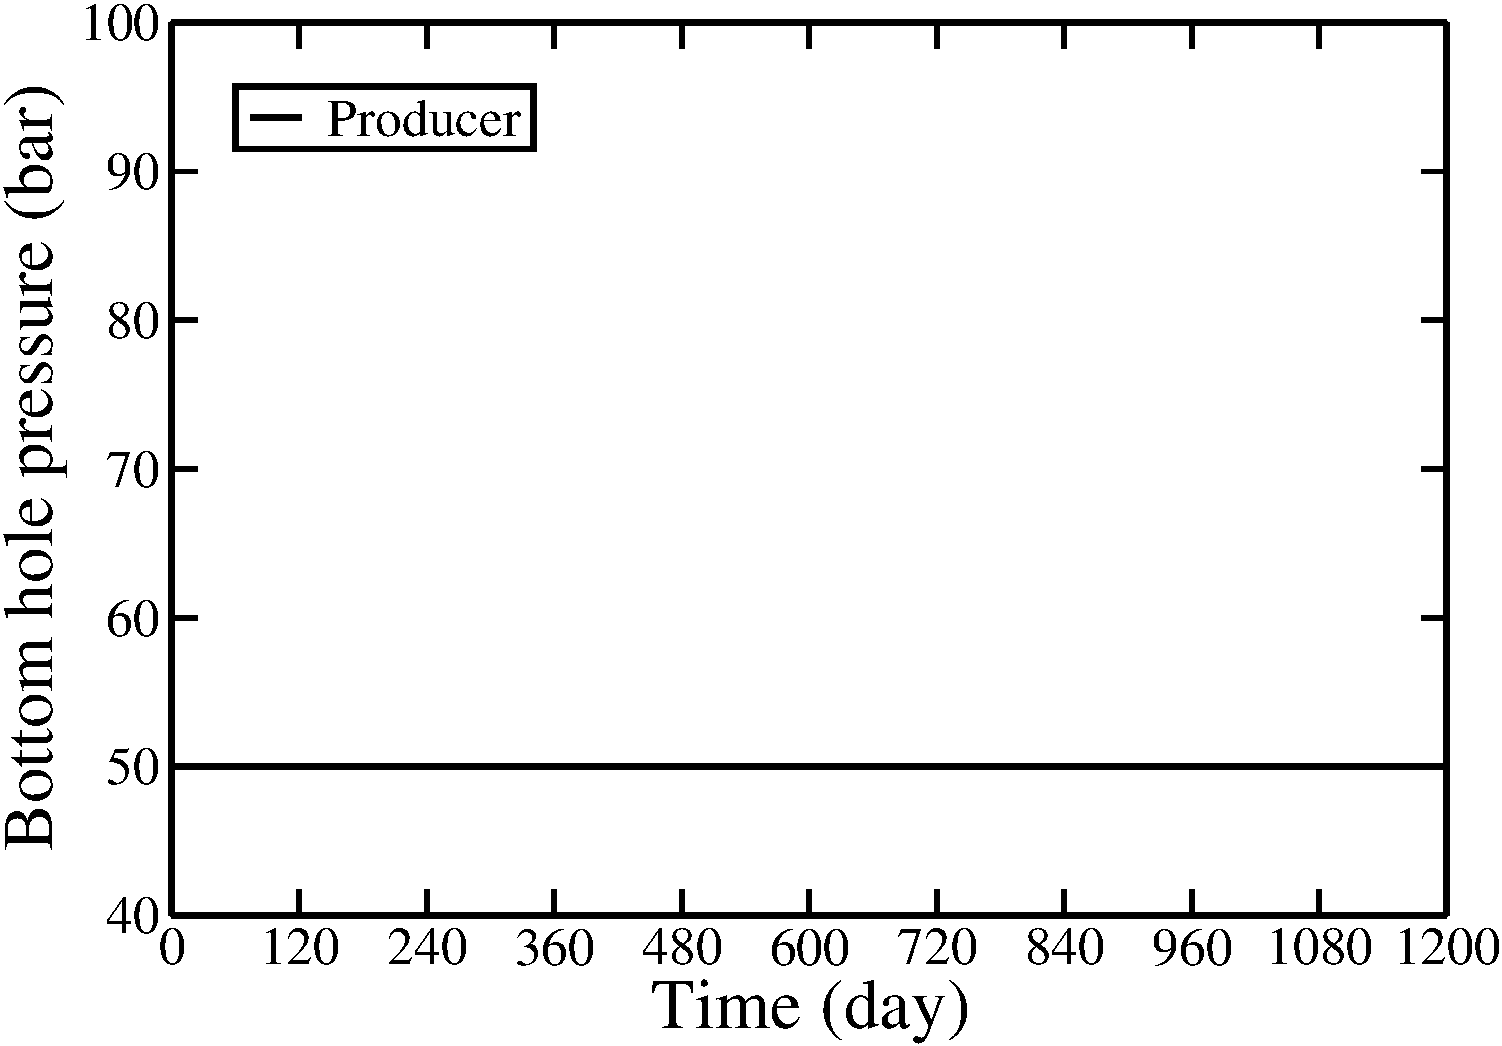
\includegraphics[height=2.7cm]{figures/SimpleBHP_BHP.pdf}
    &
    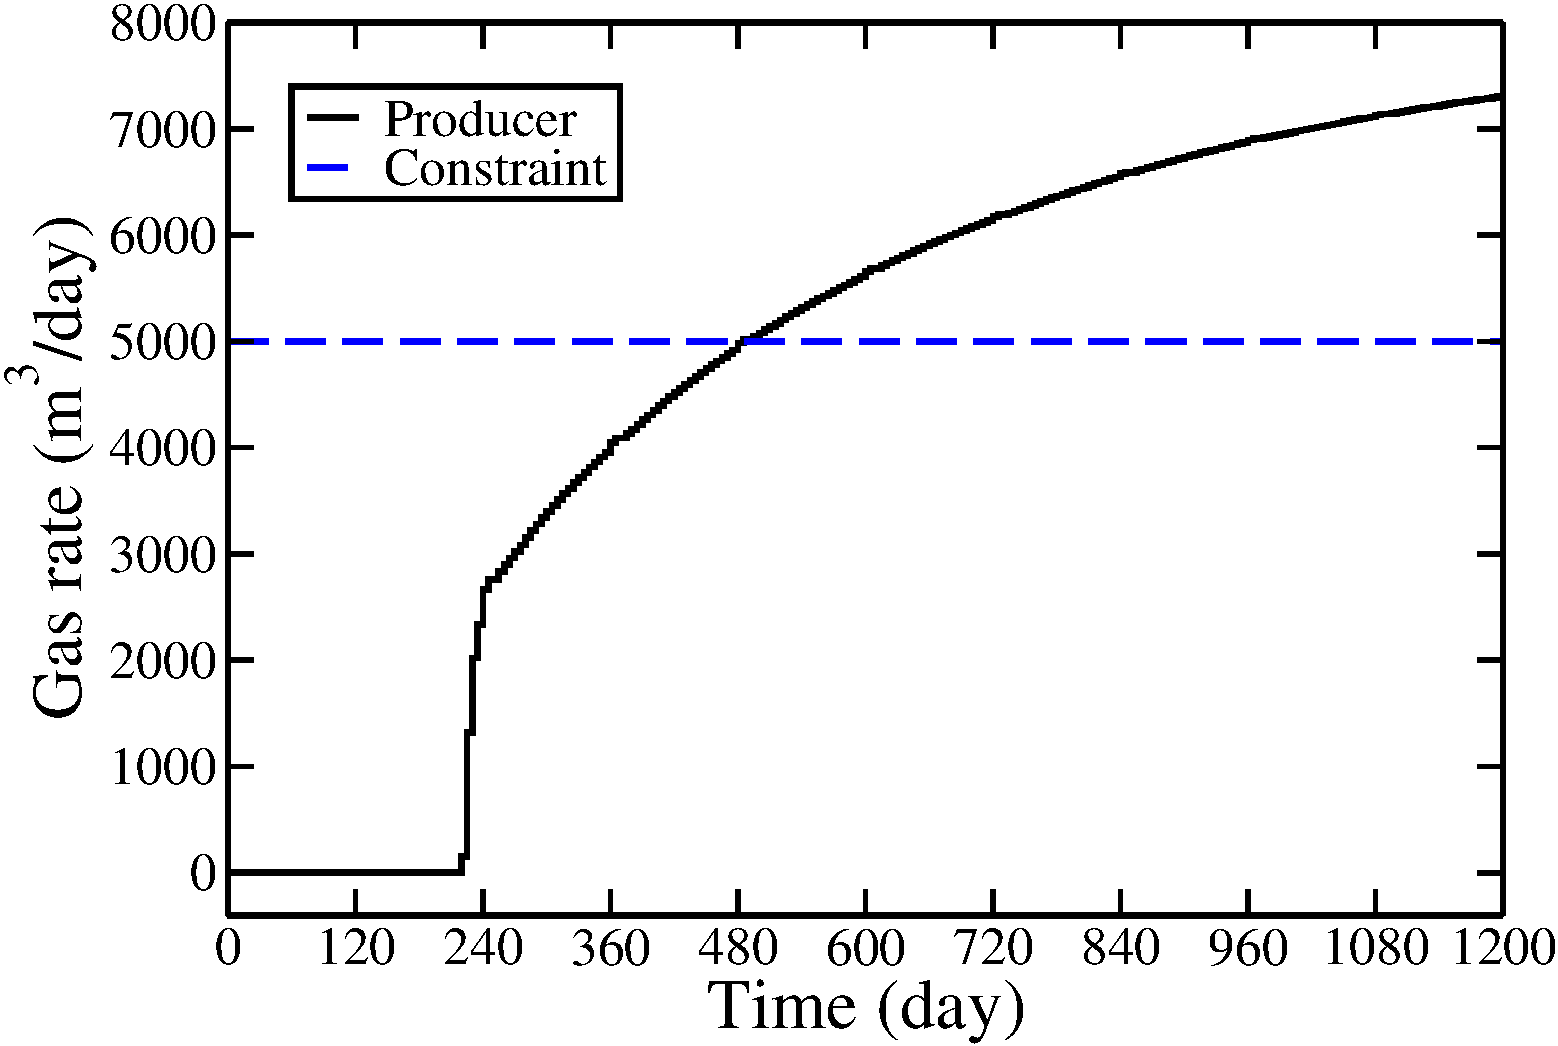
\includegraphics[height=2.7cm]{figures/SimpleBHP_rate_gas.pdf} \\
    BHP & Rate control \\
    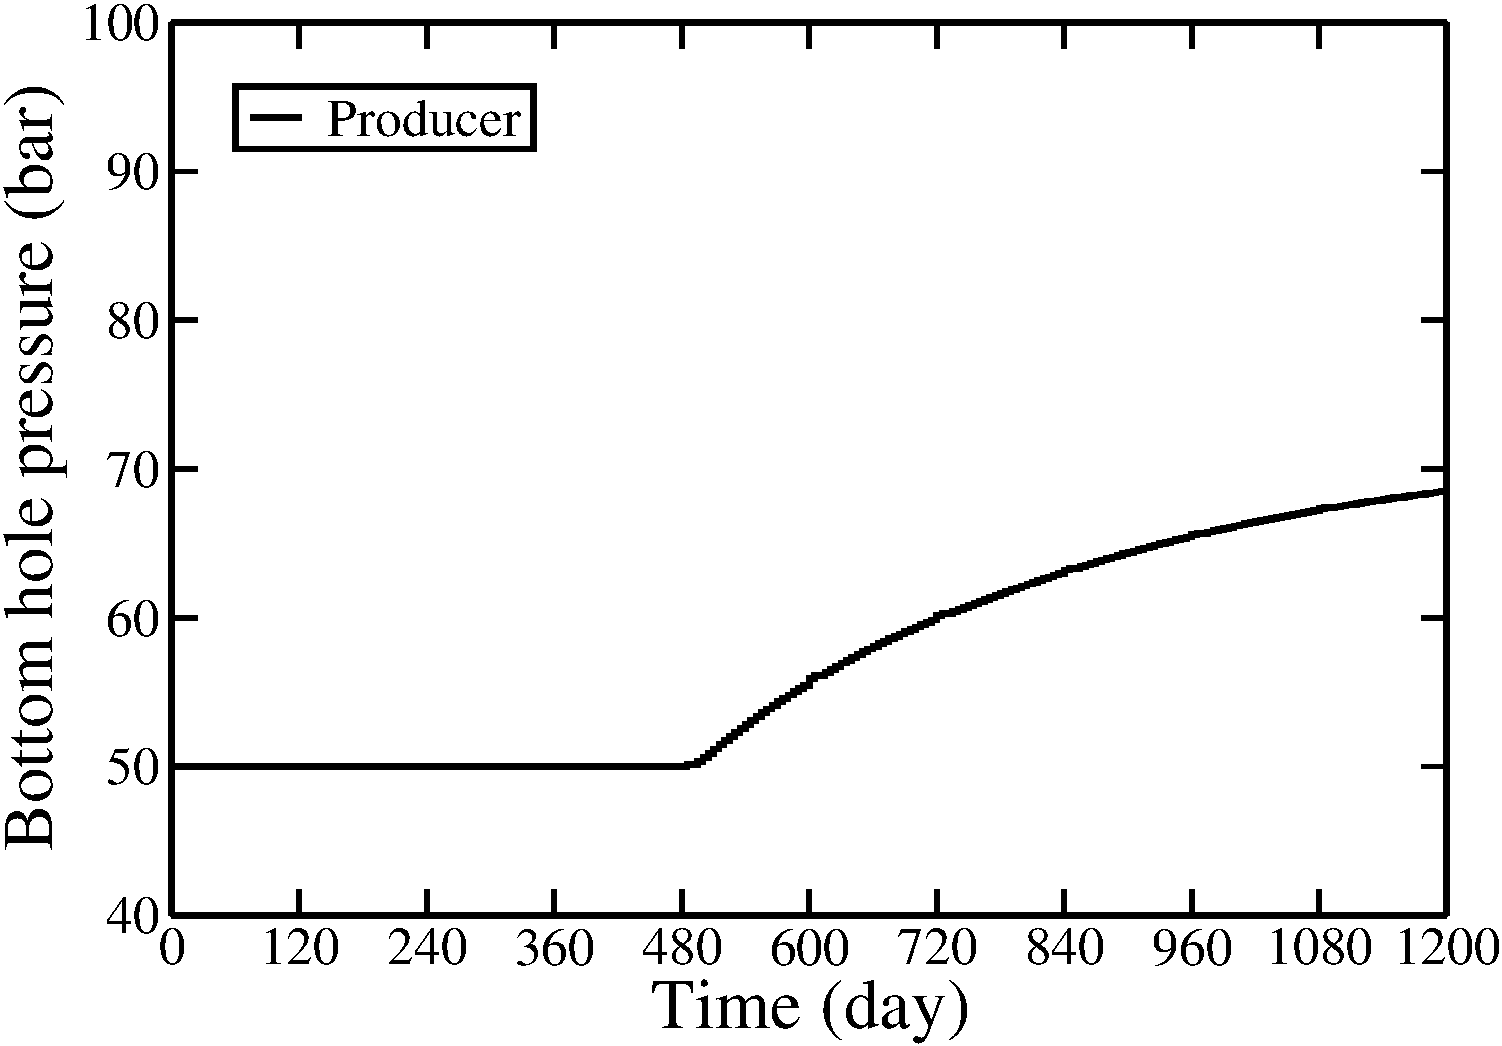
\includegraphics[height=2.7cm]{figures/SimpleRate_BHP.pdf}
    &
    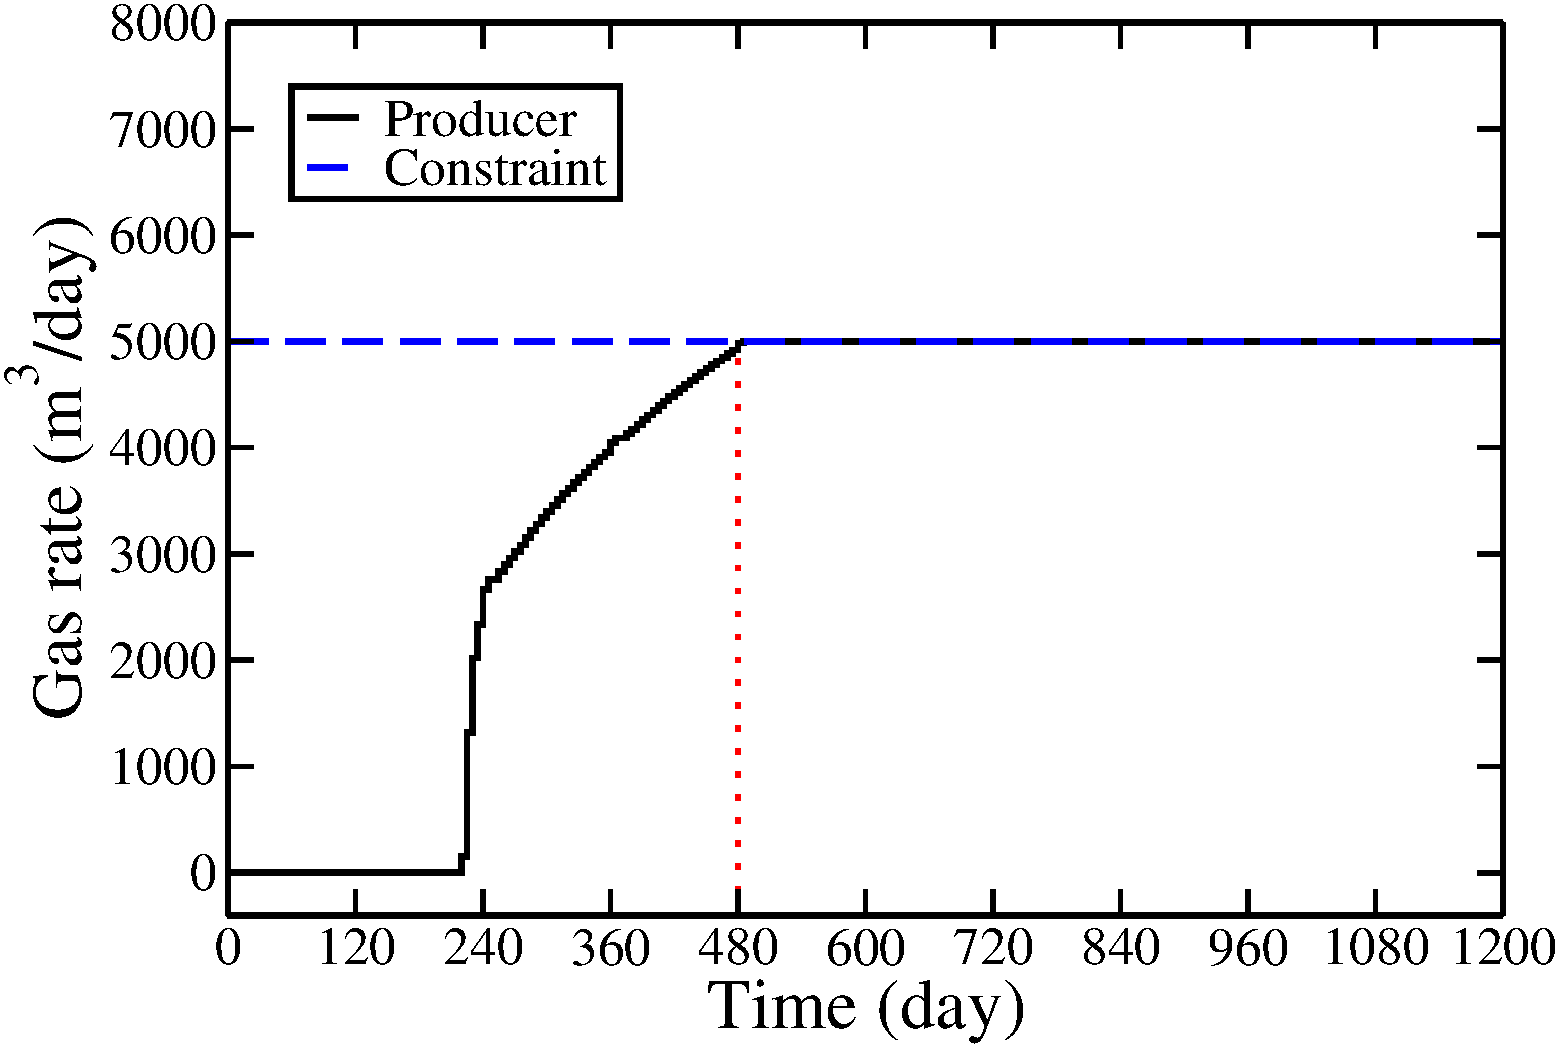
\includegraphics[height=2.7cm]{figures/SimpleRate_rate_gas.pdf} \\
  \end{tabular}
\end{center}
     \caption{Schematic illustrating heuristic constraint handling. Top: Constant BHP and resulting gas rate. Bottom: BHP and gas rate satisfying constraint.}
\label{fig:BHPvsRateControl}
\end{figure}


Although it is clearly approximate, this heuristic constraint handling approach
has some potential advantages over the formal method described in
Section~\ref{sec:constr-opt}. For example, the heuristic treatment allows the
simulator to switch controls at any time step in the simulation, while the
formal approach only allows controls to switch at a relatively small number of
control steps (by way of comparison, in a typical problem we may have
  $O(10^2-10^3)$ time steps but only $O(10)$ control steps). The heuristic
approach thus enables, in some sense, a more `fine-grained' response, and it can
be viewed as having many more `control' variables (though these variables are
  not optimized formally). Increasing the number of control steps to provide the
same granularity to the optimizer as in the forward problem (i.e., setting the
  control step size to equal the time step size) should theoretically result in
better performance by the formal approach, though in practice the large
increase in the number of control variables would result in a more difficult optimization
problem, which could negatively impact the performance of the optimizer. In the examples
below, we will compare the performance of these two approaches for handling
nonlinear constraints.

We note finally that if rates are used as the control variables, then the rate
constraints enter the optimization problem as simple bound constraints, which
are easy to satisfy. In this case, however, the BHPs become nonlinear
constraints. Our heuristic treatment would then entail the switch from rate
control to BHP control if the BHP constraint would otherwise be violated. We did
not test the performance of our procedure using rates as the control variables,
but this should be considered in future work.






%%%%%%%%%%%%%%%%%%%%%%%%%% Part One %%%%%%%%%%%%%%%%
\part{Numerical examples??}
%%%%%%%%%%%%%%%%%%%%%%%%%%%%%%%%%%%%%%%%%%%%%%%%%%%%

%%%%%%%%%%%%%%%%%%%%%%%%%%%%%%%%%%%%%%%%%%%%%%%%%
%\chapter{Constraint Handling Methods}
%%%%%%%%%%%%%%%%%%%%%%%%%%%%%%%%%%%%%%%%%%%%%%%%%
%\section{Lumping-based methods}
\chapter{Numerical results}  \label{sec:results}


We implement an adjoint treatment for multicomponent oil-gas
compositional systems through use of a recently developed automatic
differentiation capability \citep{Younis:2010}. The application of automatic
differentiation in the context of Stanford's General Purpose Research Simulator
(AD-GPRS) \citep{Cao:Thesis}, a modular simulator with many advanced features,
enables us to construct a gradient-based optimization framework suitable for
use in compositional problems. Our formulation includes the treatment of
bound, linear and nonlinear constraints. In a discrete implementation, the 
governing equations for the so-called adjoint
system are constructed based on the discretized-in-time forward model
equations. 

We will present results for four different cases. All involve bound and
nonlinear constraints, and we will compare the performance of the two approaches
described above for treating the nonlinear constraints. Because our
gradient-based optimization will find only a local optimum, we run each case
nine times, using a different initial guess for the well controls. Each initial
guess corresponds to a combination of BHPs from the set $\{p_I^u,p_I^l,p_I^a\}$
for the injectors and from the set $\{p_P^u,p_P^l,p_P^a\}$ for the producers,
where $p^u$, $p^l$ and $p^a$ designate the upper and lower limits on the
initial BHPs, and the average between these limits, respectively. We set
$p^l=p_{init}+1~{\rm bar}$ for the injectors and $p^u=p_{init}-1~{\rm bar}$
for the producers, where $p_{init}$ is the initial reservoir pressure. Note
that these `limits' are simply used to prescribe initial guesses for the
optimization -- they are not related to the actual BHP bound constraints.
For clarity, we will refer to each case by the number of the corresponding
run, as listed in Table~\ref{table:InitialGuesses}.



\begin{table}
\centering
\caption{Resulted objective values for every continuity step with respect to permeability 
for all benchmarks.}
\begin{tabular}{cccc}
\toprule
Run & SPE10TOP 1000D & SPE10TOP 3000D & Pi 256D   \\[2pt]
\midrule
1 & $5.443892E+05$ & $6.642702E+05$ & $1.252661E+05$  \\
2 & $5.631894E+05$ & $6.706731E+05$ & $1.252819E+05$ \\
3 & $5.873230E+05$  & $6.756695E+05$    & $1.244174E+05$ \\
4 & $5.986247E+05$ & $6.763321E+05$   & $1.242821E+05$ \\
5 & $5.998848E+05$  & $6.760098E+05$   & $1.241929E+05$  \\
6 & $5.962259E+05$  & $6.782397E+05$   & $1.240130E+05$   \\
7 & $5.909467E+05$  & $6.762526E+05$   & $1.242663E+05$  \\
8 & $5.850723E+05$  & $6.724442E+05$   & $1.241064E+05$  \\
9 & $5.775845E+05$  & $6.667619E+05$   & $1.240303E+05$  \\
10 & $5.688990E+05$  & $6.584114E+05$   & $1.234992E+05$   \\
11 & $5.594653E+05$  & $6.501344E+05$   & $1.229465E+05$  \\
12 & $5.507783E+05$  & $6.427540E+05$   & $1.229158E+05$  \\
13 & $5.422065E+05$  & $6.365637E+05$   & $1.226925E+05$  \\
14 & $5.339263E+05$  & $[p_I^a, p_P^a]$   & $1.225814E+05$   \\
15 & $5.256504E+05$  & $[p_I^a, p_P^a]$   & $1.221619E+05$  \\
16 & $5.180703E+05$  & $[p_I^a, p_P^a]$   & $1.217791E+05$  \\
17 & $5.120160E+05$  & $[p_I^a, p_P^a]$   & $1.214983E+05$   \\
18 & $5.071502E+05$  & $[p_I^a, p_P^a]$   & $1.212952E+05$  \\
19 & $5.044022E+05$  & $[p_I^a, p_P^a]$   & $1.211731E+05$  \\
20 & $5.033963E+05$  & $[p_I^a, p_P^a]$   & $1.211338E+05$  \\[2pt]
20* & $5.089974E+05$  & $6.018453E+05$   & $1.188555E+05$  \\[2pt]
\bottomrule
\end{tabular}
  \label{table:InitialGuesses}
\end{table}

% \begin{table}
% \centering
% \caption{Resulted objective values of the SPE10 benchmark produced for 3000 days.}
% \begin{tabular}{cc}
% \toprule
% Run & Objective value    \\[2pt]
% \midrule
% 1 & $6.642702E+05$ \\
% 2 & $6.706731E+05$ \\
% 3 & $111$ \\
% 4 & $[p_I^a, p_P^l]$ \\
% 5 & $[p_I^a, p_P^a]$ \\
% 6 & $[p_I^a, p_P^u]$ \\
% 7 & $[p_I^u, p_P^l]$ \\
% 8 & $[p_I^u, p_P^a]$ \\
% 9 & $[p_I^u, p_P^u]$ \\[2pt]
% \bottomrule
% \end{tabular}
%   \label{table:InitialGuesses}
% \end{table}
% 
% \begin{table}
% \centering
% \caption{Resulted objective values of the Pi benchmark produced for 256 days.}
% \begin{tabular}{cc}
% \toprule
% Run & Objective value    \\[2pt]
% \midrule
% 1 & $1.252661E+05$ \\
% 2 & $1.252819E+05$ \\
% 3 & $1.244174E+05$ \\
% 4c \\
% 5 & $[p_I^a, p_P^a]$ \\
% 6 & $[p_I^a, p_P^u]$ \\
% 7 & $[p_I^u, p_P^l]$ \\
% 8 & $[p_I^u, p_P^a]$ \\
% 9 & $[p_I^u, p_P^u]$ \\[2pt]
% \bottomrule
% \end{tabular}
%   \label{table:InitialGuesses}
% \end{table}
% 
% 
% 
% 
% \begin{table}
% \centering
% \caption{Initial guesses for the optimizations for all
%          cases considered.}
% \begin{tabular}{cc}
% \toprule
% Run & Initial guess    \\[2pt]
% \midrule
% 1 & $[p_I^l, p_P^l]$ \\
% 2 & $[p_I^l, p_P^a]$ \\
% 3 & $[p_I^l, p_P^u]$ \\
% 4 & $[p_I^a, p_P^l]$ \\
% 5 & $[p_I^a, p_P^a]$ \\
% 6 & $[p_I^a, p_P^u]$ \\
% 7 & $[p_I^u, p_P^l]$ \\
% 8 & $[p_I^u, p_P^a]$ \\
% 9 & $[p_I^u, p_P^u]$ \\[2pt]
% \bottomrule
% \end{tabular}
%   \label{table:InitialGuesses}
% \end{table}

\begin{figure}[htb]
\centering
\begin {tabular}{@{}cccc@{}}
 
\includegraphics[width=0.23\textwidth]{figures/VisitScreenshots/SPE1000/SPE1000_PERM_t01.png} &
 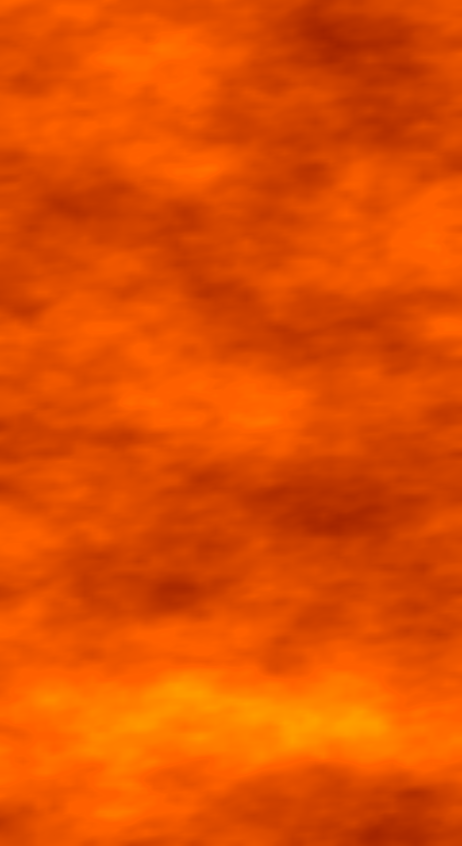
\includegraphics[width=0.23\textwidth]{figures/VisitScreenshots/SPE1000/SPE1000_PERM_t02.png} &
 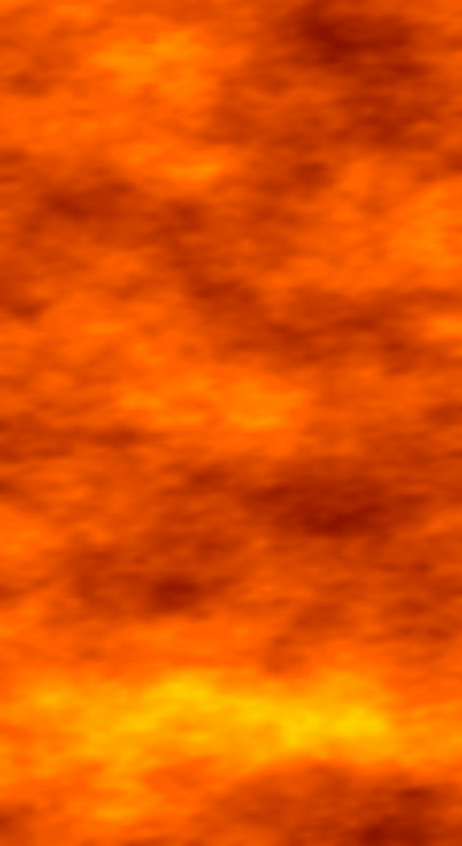
\includegraphics[width=0.23\textwidth]{figures/VisitScreenshots/SPE1000/SPE1000_PERM_t03.png} &
 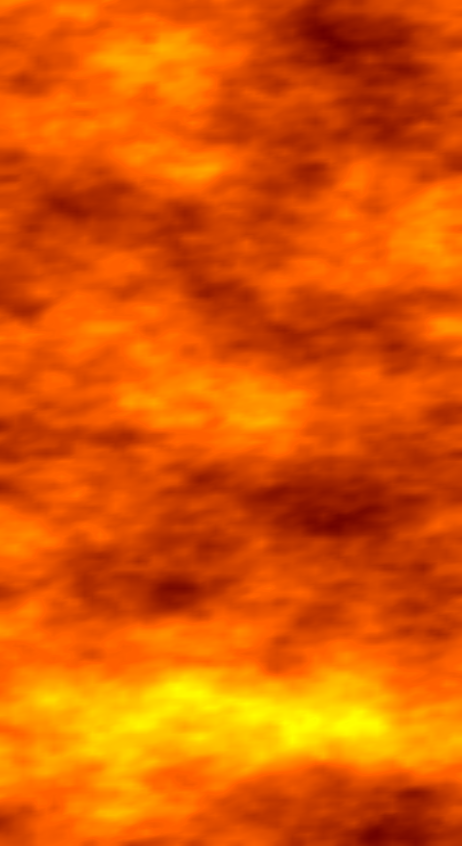
\includegraphics[width=0.23\textwidth]{figures/VisitScreenshots/SPE1000/SPE1000_PERM_t04.png} \\
 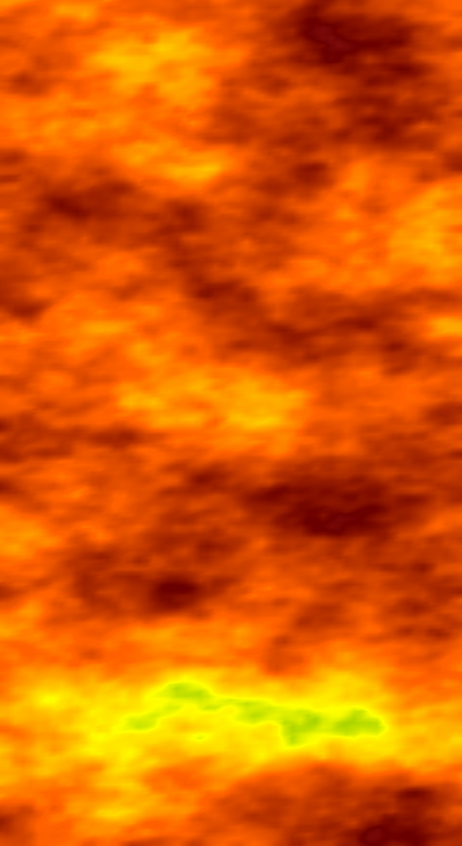
\includegraphics[width=0.23\textwidth]{figures/VisitScreenshots/SPE1000/SPE1000_PERM_t05.png} &
 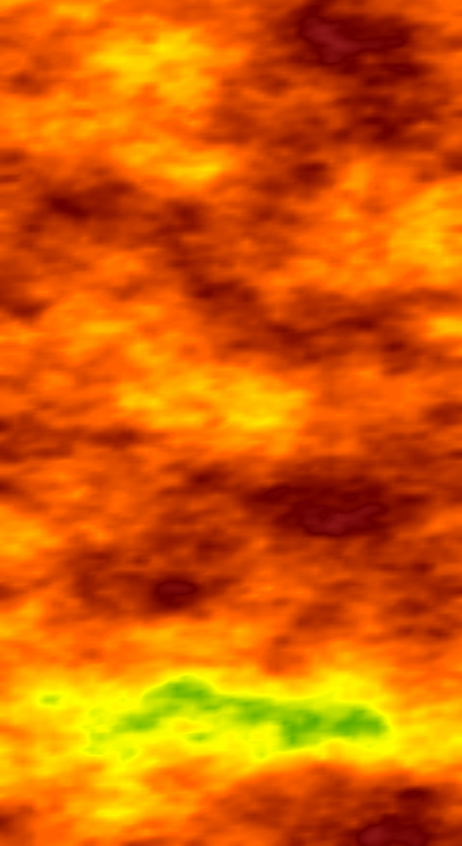
\includegraphics[width=0.23\textwidth]{figures/VisitScreenshots/SPE1000/SPE1000_PERM_t06.png} &
 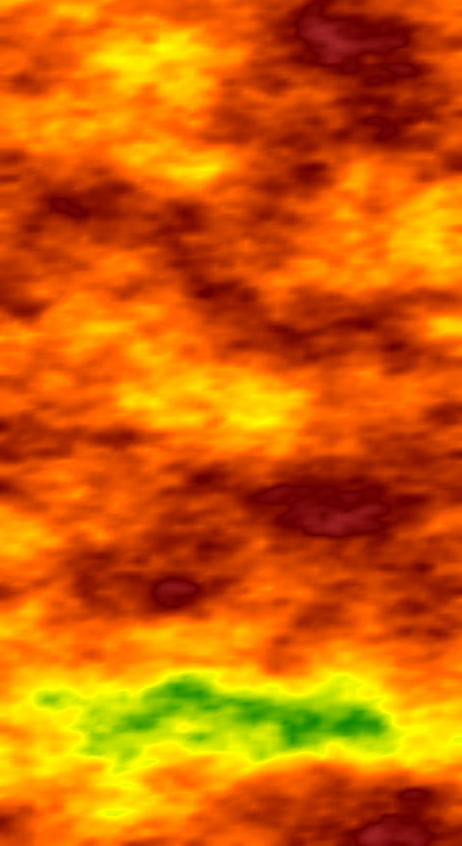
\includegraphics[width=0.23\textwidth]{figures/VisitScreenshots/SPE1000/SPE1000_PERM_t07.png} &
 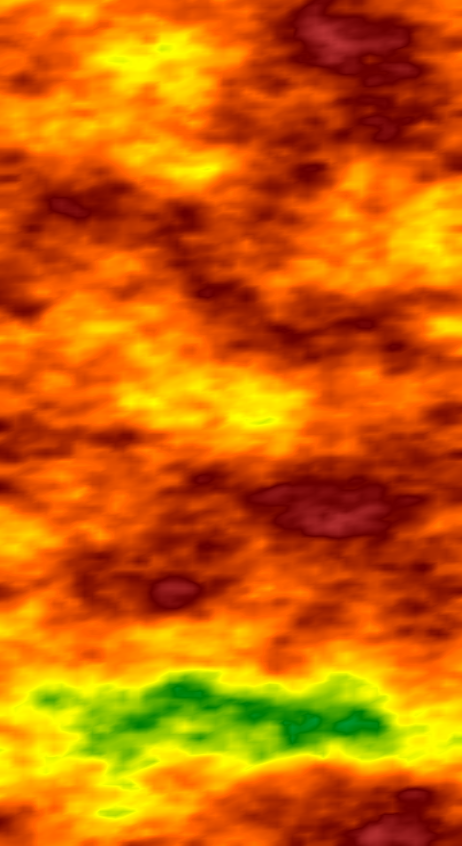
\includegraphics[width=0.23\textwidth]{figures/VisitScreenshots/SPE1000/SPE1000_PERM_t08.png} \\
 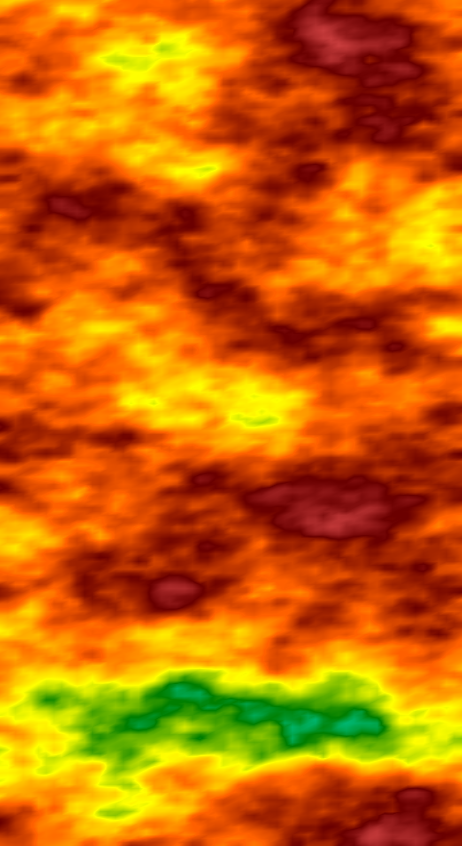
\includegraphics[width=0.23\textwidth]{figures/VisitScreenshots/SPE1000/SPE1000_PERM_t09.png} &
 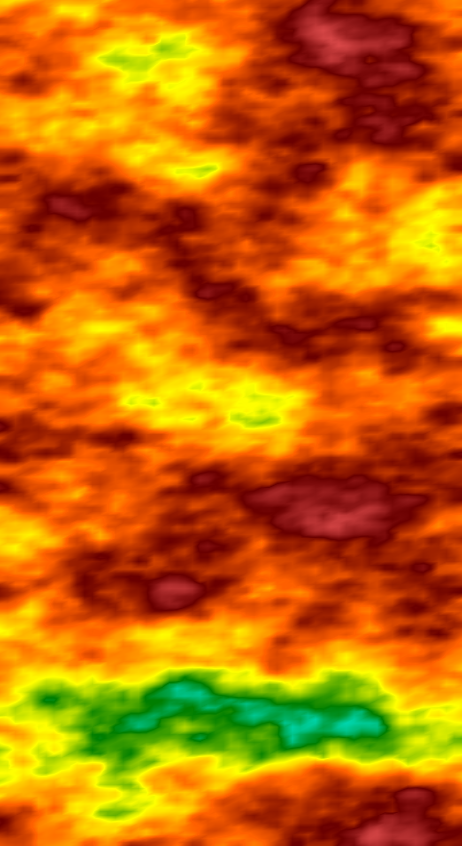
\includegraphics[width=0.23\textwidth]{figures/VisitScreenshots/SPE1000/SPE1000_PERM_t10.png} &
 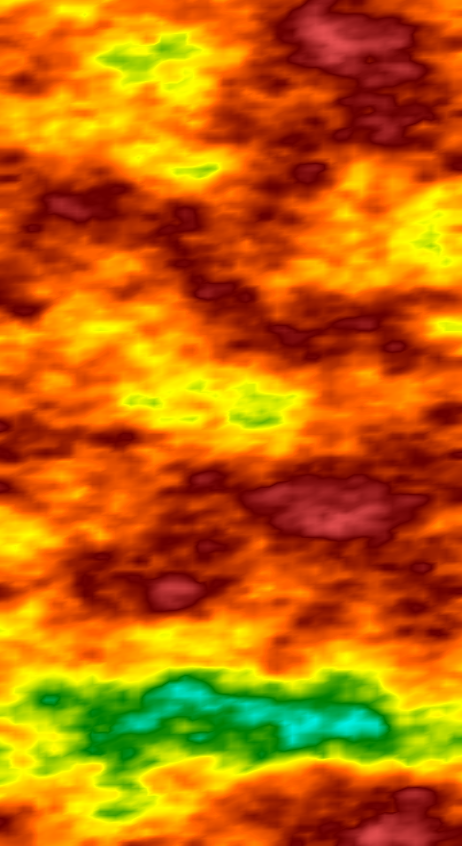
\includegraphics[width=0.23\textwidth]{figures/VisitScreenshots/SPE1000/SPE1000_PERM_t11.png} &
 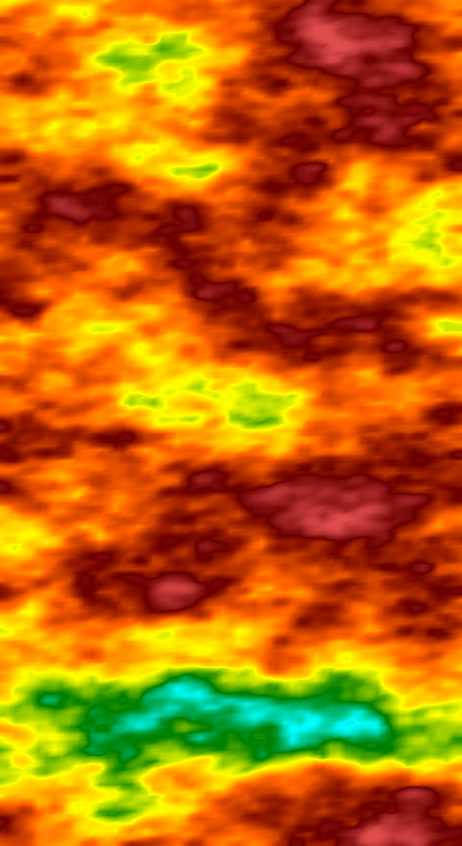
\includegraphics[width=0.23\textwidth]{figures/VisitScreenshots/SPE1000/SPE1000_PERM_t12.png} \\
 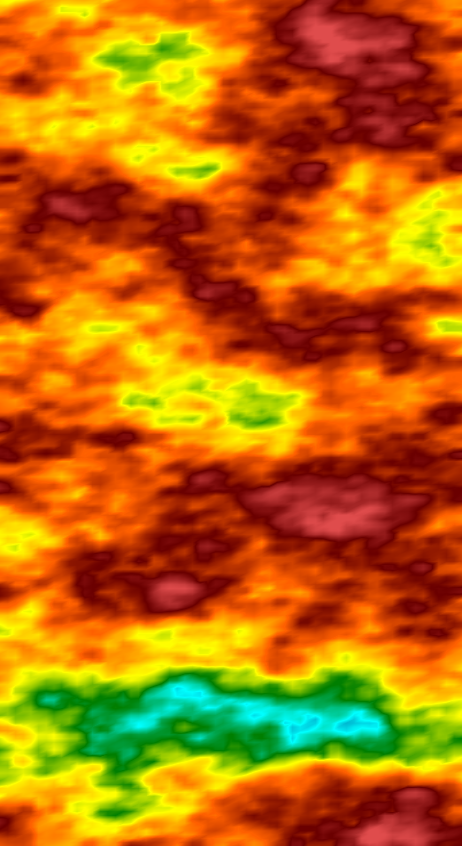
\includegraphics[width=0.23\textwidth]{figures/VisitScreenshots/SPE1000/SPE1000_PERM_t13.png} &
 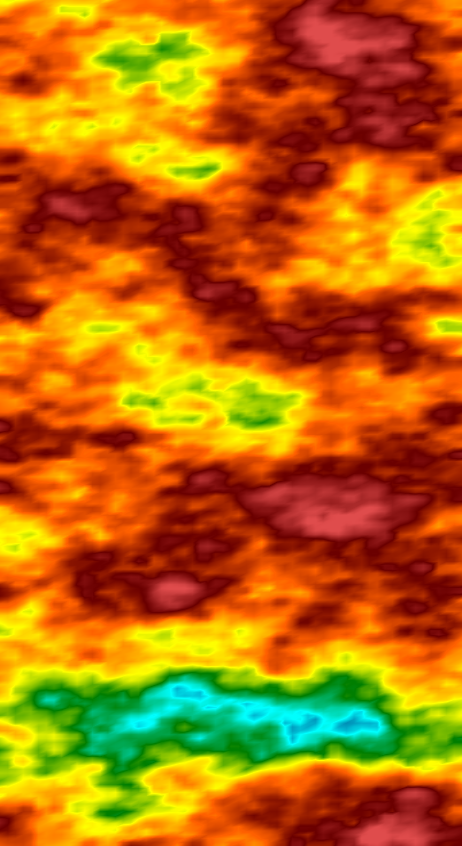
\includegraphics[width=0.23\textwidth]{figures/VisitScreenshots/SPE1000/SPE1000_PERM_t14.png} &
 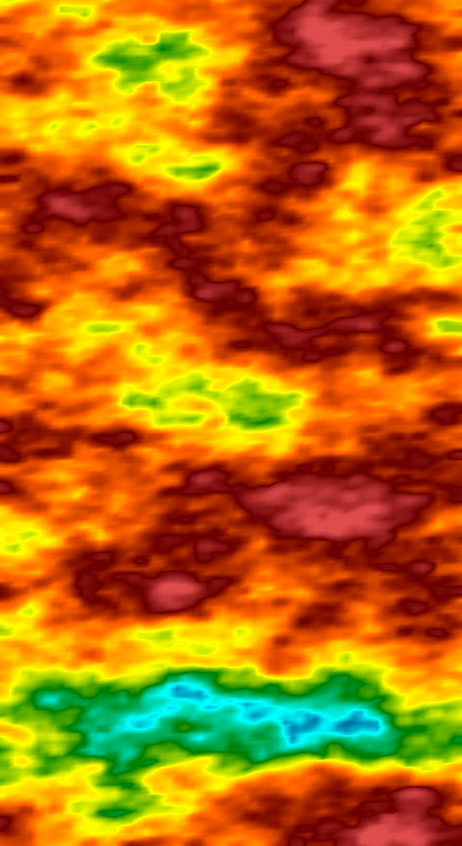
\includegraphics[width=0.23\textwidth]{figures/VisitScreenshots/SPE1000/SPE1000_PERM_t15.png} &
 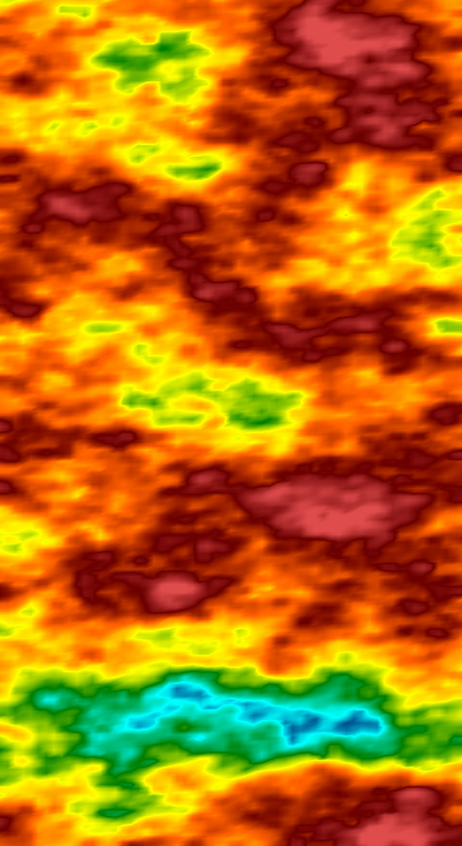
\includegraphics[width=0.23\textwidth]{figures/VisitScreenshots/SPE1000/SPE1000_PERM_t16.png} \\
%  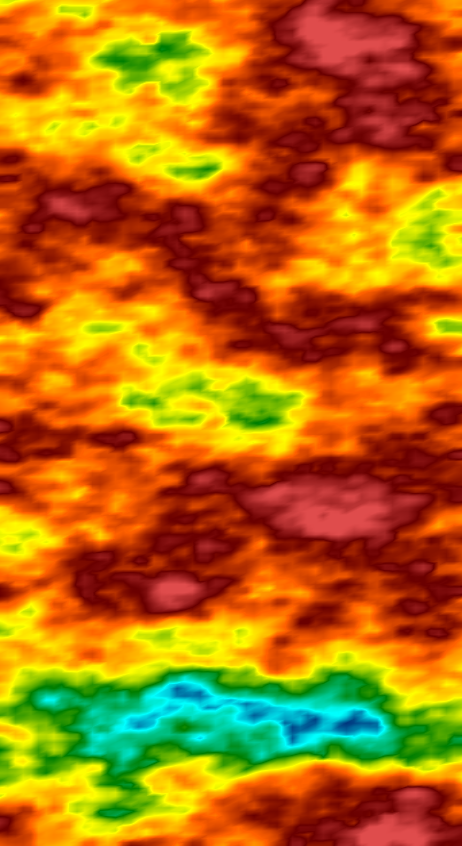
\includegraphics[width=0.23\textwidth]{figures/VisitScreenshots/SPE1000/SPE1000_PERM_t17.png} &
%  
\includegraphics[width=0.23\textwidth]{figures/VisitScreenshots/SPE1000/SPE1000_PERM_t01.png} &
%  
\includegraphics[width=0.23\textwidth]{figures/VisitScreenshots/SPE1000/SPE1000_PERM_t01.png} &
%  
\includegraphics[width=0.23\textwidth]{figures/VisitScreenshots/SPE1000/SPE1000_PERM_t01.png} \\
\multicolumn{4}{c}%{ 
\includegraphics[width=0.23\textwidth]{figures/VisitScreenshots/SPE1000/SPE1000_PERM_t01.png} }

\end {tabular}
\caption {hgchgm}

% \begin{subfigure}{0.5\textwidth}
% 
\includegraphics[width=0.9\linewidth, height=5cm]{figures/VisitScreenshots/SPE1000/SPE1000_PERM_t01.png} 
% \caption{Permeability}
% \label{fig:subim1}
% \end{subfigure}
% \begin{subfigure}{0.5\textwidth}
% 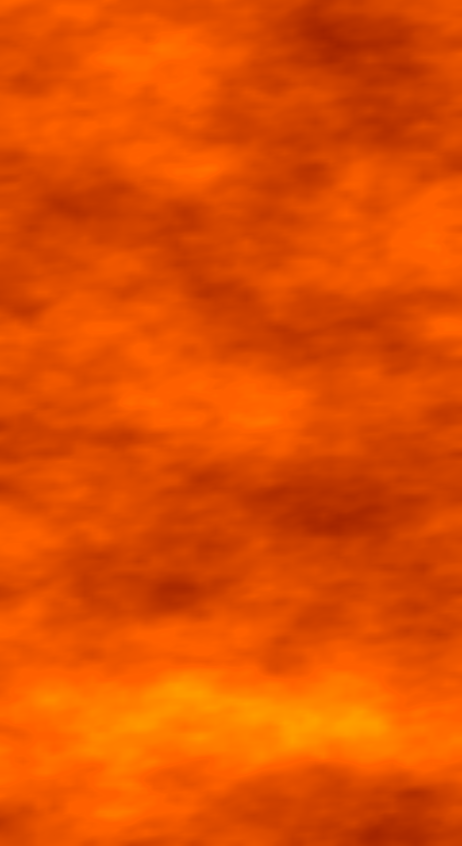
\includegraphics[width=0.9\linewidth, height=5cm]{figures/VisitScreenshots/SPE1000/SPE1000_PERM_t02.png}
% \caption{Oil saturation}
% \label{fig:subim2}
% \end{subfigure}
% \begin{subfigure}{0.5\textwidth}
% 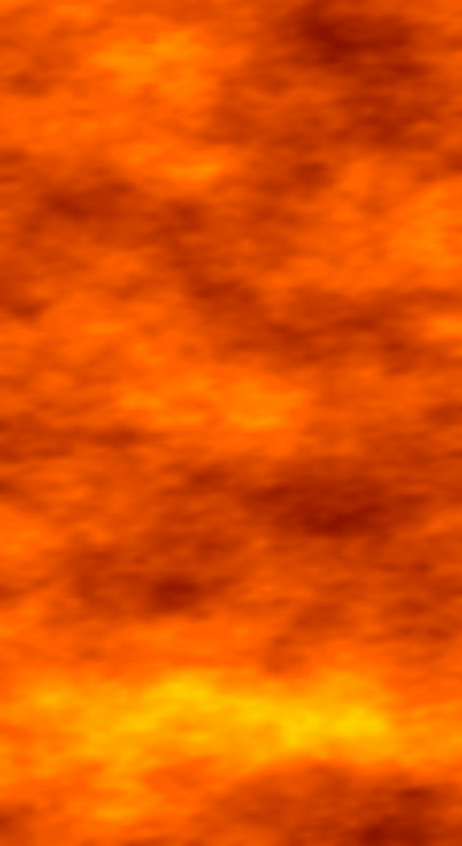
\includegraphics[width=0.9\linewidth, height=5cm]{figures/VisitScreenshots/SPE1000/SPE1000_PERM_t03.png}
% \caption{Oil saturation}
% \label{fig:subim2}
% \end{subfigure}
% \caption{Step 1 out of 20 for the SPE10 top layer, after 3000 days, .}
% \label{fig:image2}
 \end{figure}



\subsection{Example 1 - $\Pi$ obstacle}

In the first example we maximize cumulative oil recovery under CO$_2$ injection. The two-dimensional geological model is depicted in Fig.~\ref{fig:PImodelPermeabilityMapAndWells}. A $\Pi$-shaped region is located at the center of a homogeneous reservoir. The model is discretized on a grid of dimensions $80\times80$. The permeability in most of the domain (red cells) is set to 4000~mD, while the permeability for the blue cells that comprise the $\Pi$-shaped region is set to $10^{-4}$~mD. In all of our examples we describe the permeability with a diagonal tensor: $\tens{K} = \it{diag}(\tens{k}_x, \tens{k}_y, \tens{k}_z)$; here, in addition, the permeability is isotropic and uniform within each of the regions. Four injection wells are placed at the corners of the model, and the single production well is located inside the $\Pi$-shaped region. The model includes a total of four components (three hydrocarbon  components plus CO$_2$), as specified in Table~\ref{table:fluidForPImodel}. Further details on the reservoir model are provided in Table~\ref{table:PI}.

%
\begin{table}
\centering
\caption{Fluid description for Example 1}
\begin{tabular}{|l|r|r|r|r|}
\hline
Component            & CO$_2$ & C$_1$ & C$_4$ & C$_{10}$    \\
\hline
Initial composition (\%)  & 1    & 20  & 29    & 50 \\
Injection composition (\%)& 100   & - & - & - \\
\hline
\end{tabular}
\label{table:fluidForPImodel}
\end{table}
%

%
\begin{table}
\tabcolsep=0pt
\centering
\caption{Model parameters for example 1.}
\label{table:PI}
\begin{tabular*}{84mm}{@{\extracolsep\fill}lll}\toprule
Parameter                & Value    & Units \\
\midrule
Grid size                & 80 $\times$ 80 $\times$ 1 &  ---  \\
$\Delta x$               & 6 &m          \\
$\Delta y$               & 6 &m          \\
$\Delta z$               & 4&m         \\
Depth                    & 4000&m           \\
Initial pressure         & 100  & bar        \\
Temperature              &$100$ & $^\circ$C     \\
Rock compressibility     & $7.2 \times 10^{-5}$ & 1 / bar \\
Simulation time          &256 & d           \\
Pressure upper bound     & 120 & bar        \\
Pressure lower bound     &  90 & bar        \\
Residual gas saturation  & 0 & ---          \\
Residual oil saturation  & 0 & ---          \\ 
 End point rel perm gas   & 1 & ---          \\
End point rel perm oil   & 1 & ---          \\
Corey exponent gas       & 2 & ---          \\
Corey exponent oil       & 2 & ---          \\[2pt]
\bottomrule
Well locations [grid block no.] & $i$ & $j$ \\
\midrule
Injector 1               &   1&  1   \\
Injector 2               &   1& 80   \\
Injector 3               &  80&  1   \\
Injector 4               &  80& 80   \\
Producer 1               &  40& 48   \\[2pt]
\bottomrule
\end{tabular*}
\end{table}
%



The control parameters in the optimization problem are the well BHPs. These are constrained to lie between an
upper bound of 120~bar and a lower bound of 90~bar. We additionally specify a
maximum (per-well) gas injection rate of 500~m$^3/$d at reservoir conditions.
The total simulation period is 256~days, and the well controls are determined
at initial time and for every subsequent 32-day interval. There are thus a
total of eight control steps and 40 control parameters.

Two reference solutions are generated. First, we run the
simulation with the production wells operating at the minimum BHP and the
injection wells at the maximum BHP. This solution is infeasible because it
violates the nonlinear output constraints (maximum gas injection rate of 500~m$^3/$d). Next, we apply the heuristic
constraint handling approach described above, with the maximum gas injection
rate set to 500~m$^3/$d. The cumulative oil production for these two cases is
given in the first row (`Reference') of Table~\ref{table:PiC500Steps8}. 
The table headings refer to the treatment of the
nonlinear constraints -- bound constraints are satisfied in all cases.


We next perform optimizations that honor the bound constraints but not the
nonlinear constraints. The results for the nine runs, starting from different
initial guesses, are presented in Table~\ref{table:PiC500Steps8} in the column
labeled `Unconstr.' The best optimum achieved is a cumulative oil production of 190,200~m$^3$, obtained in Run~7.  This clearly exceeds the unconstrained reference result
of 163,900~m$^3$. Results using heuristic constraint handling are shown in
the third column. Here the best result is a cumulative oil production of 163,500~m$^3$ (Run~8), which exceeds the feasible reference solution (152,200~m$^3$) by 7.4\%. In the next set of runs we apply the formal constraint handling treatment. For
these runs, the best optimum is 160,600~m$^3$ of oil (Run~4). This value exceeds the feasible reference solution by 5.5\%, but it is about 2\% less than that achieved using heuristic constraint handling. We will show below that results using the formal procedure can be improved through use of more control steps.


The oil production profiles for the best runs, along with the reference
(heuristic) case, are shown in Fig.~\ref{fig:PIRevenue}. Recall that
we are maximizing cumulative oil, so the fact that early time production in the
reference case exceeds that of the optimized cases is not of concern. The
detailed BHP and gas rate profiles for each case are shown in Figs.~\ref{fig:PIReferencePlots},
\ref{fig:PIHeuristicControls40Plots} and \ref{fig:PIFormalControls40Plots}. The oil rates for all three cases are depicted in Fig.~\ref{fig:PIOilRates}. Although the BHPs for the two
optimized cases are clearly different, the oil rate profiles do show some general
similarity. For example, they both show less variation in oil rate over the course of the simulation than the reference case.

It is important to note that the heuristic constraint handling approach is
more efficient computationally than the formal treatment. In terms of computational requirements, for this case the formal approach required 49 forward simulations (on average) to converge to the optimal solution, while the heuristic procedure needed only an average of 27 forward simulations. This significant difference results from the need to enforce feasibility within the optimizer in the formal constraint handling approach.


We now assess the impact of using additional control variables. Theoretically, if the optimization problem remains sufficiently `tractable', as we increase the number of control variables the formal approach should (eventually) outperform the heuristic approach. However, if the optimization problem becomes significantly more difficult with increasing numbers of control variables (which may be related to the constraint lumping procedure), or if a large number of local optima associated with relatively poor objective function values appear, then the formal approach will not necessarily outperform the heuristic treatment. 

To test the performance of our procedures, we now consider optimizations with 64 control steps, which corresponds to 320 control variables (the results above used eight control steps and 40 control variables). Results for this case are presented in Table~\ref{table:PiC500Steps64}. The best result using heuristic constraint handling provides cumulative oil production of 159,400~m$^3$ (Run~7). This is slightly lower than that achieved using 40 controls, which presumably reflects the fact that this is a more difficult optimization problem. Using the formal constraint handling approach, however, we achieve cumulative oil production of 170,200~m$^3$ (Run~1). This exceeds the feasible reference solution (152,500~m$^3$) by 11.6\%, which represents a substantial improvement. It also exceeds the best solution found using heuristic constraint handling (163,500~m$^3$ in Run~8, using 40 controls) by 4.1\%. In fact, three of the nine local optima achieved in this case using formal constraint handling exceed the best result obtained using heuristic constraint handling. These findings suggest that, for this problem, the formal approach does indeed outperform the heuristic approach given a sufficient number of control variables. 


Finally, it is worth noting that the spread in the results from run to run for (optimized) cumulative oil is larger with 320 control variables than it is with 40 control variables. In fact, with 320 control variables, optimizations using both constraint handling procedures lead to some local optima that are below the corresponding lowest optima achieved using 40 control variables (Runs~3 and 5 for the heuristic approach; Runs~2, 3 and 4 for the formal approach). Again, we believe this is indicative of the challenges associated with performing constrained optimization with increasing numbers of control variables. These results suggest that it may be useful to explore the use of a sequence of optimizations, with increasing numbers of control periods, for production optimization problems.


\pgfplotstableset{% global config, for example in the preamble
        % these columns//.style={} things define a style
        % which applies to  only.
        columns/Run/.style={int detect,column type=r,column name=\textsc{Run}},
        columns/Unconstr./.style={column name=\textsc{Unconstr},fixed,sci zerofill,column type=r,sci sep align,precision=1,string replace={--}{}},
        columns/Heuristic/.style={column name=\textsc{Heuristic},fixed,sci zerofill,column type=r,sci sep align,precision=1,string replace={--}{}},
        columns/Formal/.style={column name=\textsc{Formal},fixed,sci zerofill,column type=r,sci sep align,precision=1,string replace={--}{}},
        empty cells with={--},
        every head row/.style={before row=\toprule,after row=\midrule},
        every last row/.style={after row=\bottomrule}
}
\begin{table}
\centering
\pgfplotstabletypeset[
columns={Run,Unconstr.,Heuristic,Formal},
]{Pi40.dat}
\caption{Oil production in $10^3$~m$^3$ (Example 1, {\bf 40 control variables}) for the optimized objective function
         without satisfying the nonlinear constraints (`Unconstr.'), satisfying the nonlinear constraints
         using the heuristic treatment (`Heuristic'), and satisfying the nonlinear constraints
         using the formal approach (`Formal'). Best feasible results shown in bold.}
\end{table}       

\begin{figure}[ht]
\begin{center}
     \begin{tabular}{cccccccc}
      0.0001 &  500 & 1000 & 1500 & 2000 & 2500 & 3000 &4000
      \end{tabular}
      
\includegraphics[width=8cm, height=0.5cm]{figures/VanEssenModelPermeabilityMapColorBar.png}
       
       \medskip

       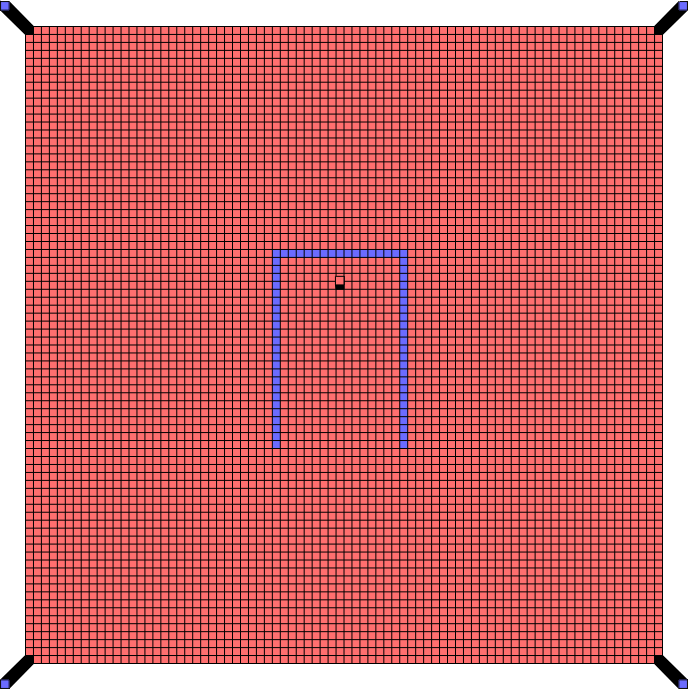
\includegraphics[totalheight=3.in]{figures/PiPermeabilityMapAndWells.png} 
       \end{center}
     \caption{Injection wells (blue) and production well (red) for Example~1. Background shows $\tens{k}_x$ ($ \tens{k}_x = \tens{k}_y$).}
  \label{fig:PImodelPermeabilityMapAndWells}
\end{figure}



\begin{table}
\centering
\caption{Oil production in $10^3$~m$^3$ (Example 1, {\bf 40 control variables}) for the optimized objective function
         without satisfying the nonlinear constraints (`Unconstr.'), satisfying the nonlinear constraints
         using the heuristic treatment (`Heuristic'), and satisfying the nonlinear constraints
         using the formal approach (`Formal'). Best feasible results shown in bold.}
\begin{tabular}{|c|c|c|c|}
\hline
   Run & Unconstr. & Heuristic & Formal                       \\
\hline
Reference    & 163.9         &  152.2                      &                           \\
1                     & 187.5         &  156.6                      &        158.2        \\
2                     & 189.1         &  162.0                      &        146.2        \\
3                     & 177.3         &  149.0                      &        149.2        \\
4                     & 183.4         &  150.2                      & \bf{ 160.6 }      \\
5                     & 186.1         &  152.2                      &        152.9        \\
6                     & 185.0         &  158.9                      &        160.2        \\
7                     & 190.2         &  162.3                      &        142.5        \\ 
8                     & 190.1         &\bf{163.5}                 &        158.5        \\
9                     & 190.1         &     162.0                   &        158.0        \\
\hline
\end{tabular}
  \label{table:PiC500Steps8}
\end{table}


   
          
             
\begin{table}
\centering
\caption{Oil production in $10^3$~m$^3$ (Example 1, {\bf 320 control variables}) for the optimized objective function
         without satisfying the nonlinear constraints (`Unconstr.'), satisfying the nonlinear constraints
         using the heuristic treatment (`Heuristic'), and satisfying the nonlinear constraints
         using the formal approach (`Formal'). Best feasible results shown in bold.}
\begin{tabular}{|c|c|c|c|}
\hline
   Run & Unconstr. & Heuristic & Formal                          \\
\hline
Reference             & 150.1         &  152.5                      &                     \\
1                     & 188.1         &  149.9                      &  \bf{ 170.2 }        \\
2                     & 192.4         &  155.6                      &         131.4            \\
3                     & 186.5         &  136.4                      &         117.8          \\
4                     & 186.8         &  149.9                      &         133.7          \\
5                     & 186.5         &  142.2                      &         156.1          \\
6                     & 192.5         &  157.8                      &         168.2          \\
7                     & 192.5         &  \bf{159.4}               &         158.8          \\ 
8                     & 192.4         &  156.9                      &         161.1          \\
9                     & 192.2         &  157.0                      &         165.8          \\
\hline
\end{tabular}
  \label{table:PiC500Steps64}
\end{table}
 
 
 
 

 



%\begin{figure}[htb]
%\begin{center}
%     \begin{tabular}{ccccccccc}
%      0 &  0.125 & 0.250 & 0.375 & 0.500 & 0.625 & 0.750 & 0.875 & 1
%      \end{tabular}
%      
\includegraphics[width=8cm, height=0.5cm]{VanEssenModelPermeabilityMapColorBar.png}
%       
%       \medskip
%
%       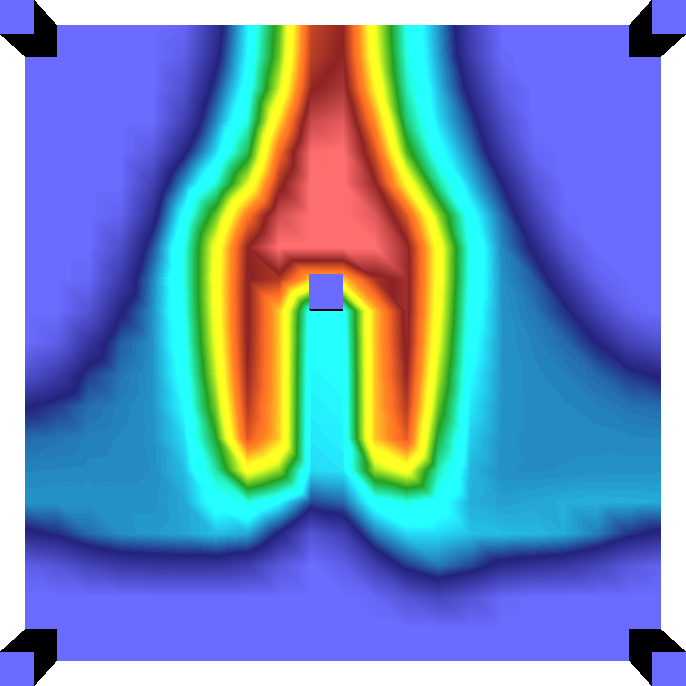
\includegraphics[totalheight=3.in]{PiBenchmarkSteps256RefenceC500T256.png} 
%
%       \medskip
%
%       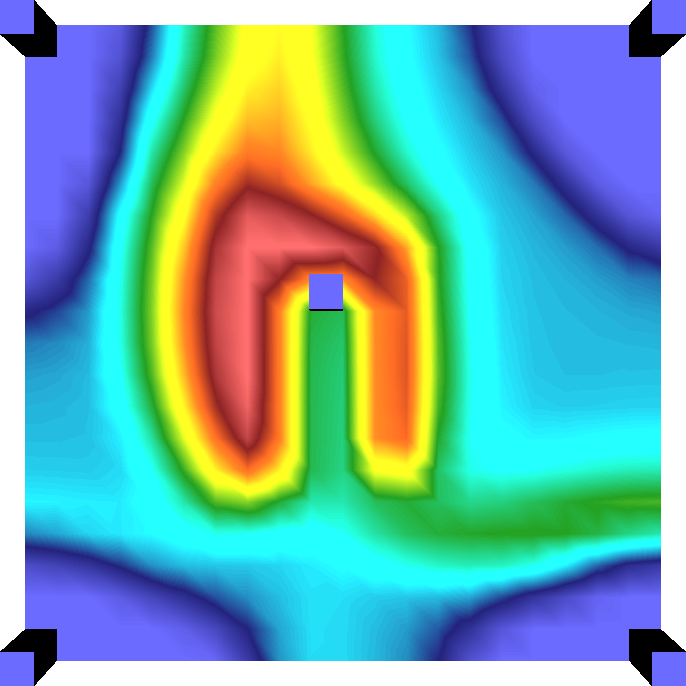
\includegraphics[totalheight=3.in]{PiBenchmarkSteps256HeuristicC500T256.png} 
%
%       \medskip
%
%       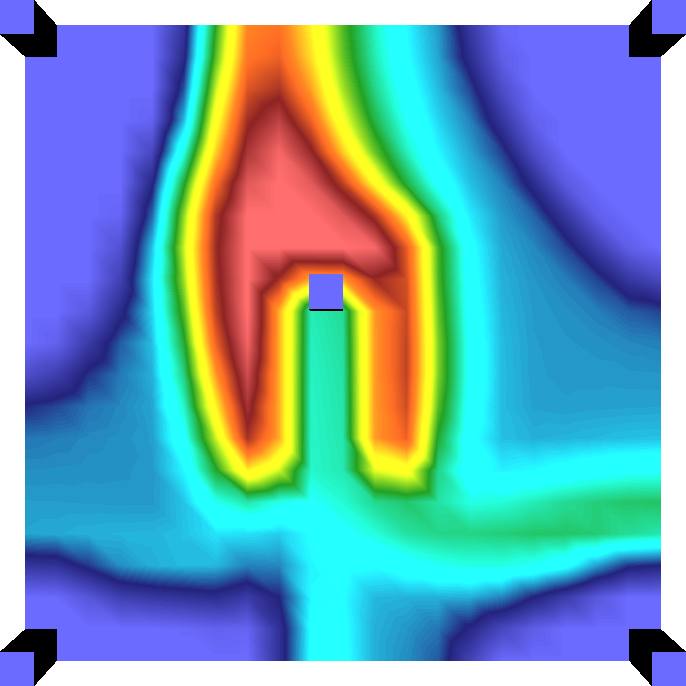
\includegraphics[totalheight=3.in]{PiBenchmarkSteps256FormalC500T256.png} 
%
%       \end{center}
%     \caption{Injection wells (blue) and production wells (red) for Example 1. Background shows $\tens{K}_x$ ($ \tens{K}_x = \tens{K}_y$).}
%  \label{fig:PImodelOilSaturation}
%\end{figure}

\begin{figure} [ht]
\begin{center}
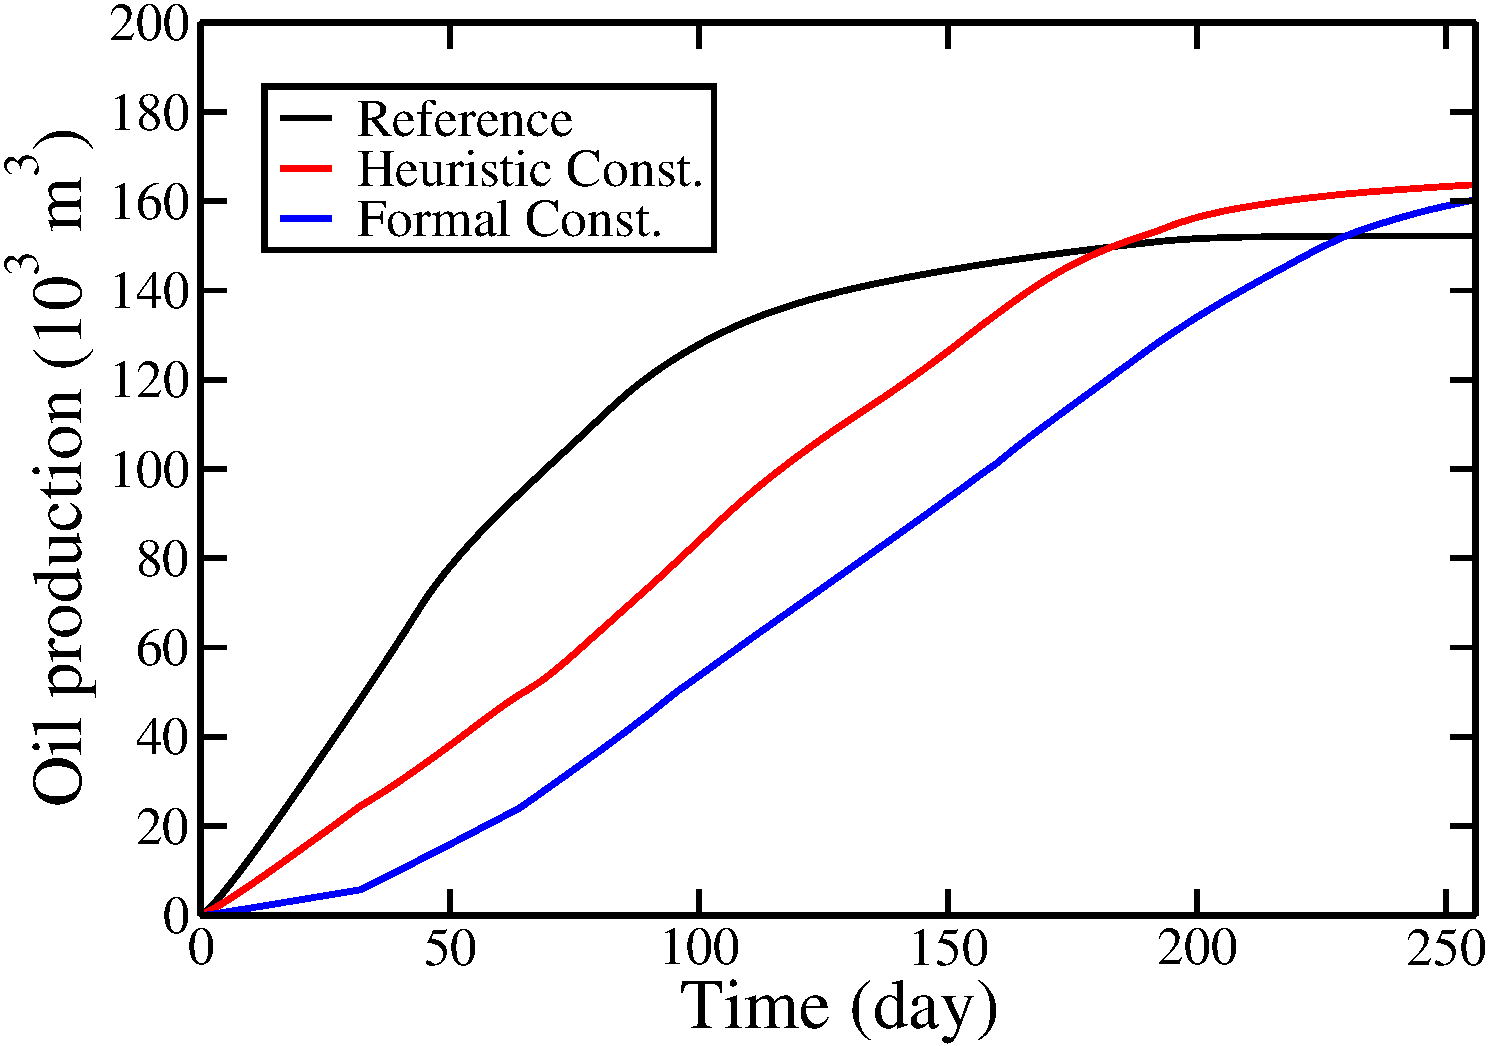
\includegraphics[totalheight=2.17in,angle=0]{figures/RevenuePI2.pdf}
\end{center}
\caption{Oil production versus time (Example 1, 40 control variables). Results are for
  feasible reference case (black curve), best heuristically constrained solution (Run 8, red curve)
  and best formally constrained solution (Run 4, blue curve).}
\label{fig:PIRevenue}
\end{figure}
\begin{figure}
\begin{center}
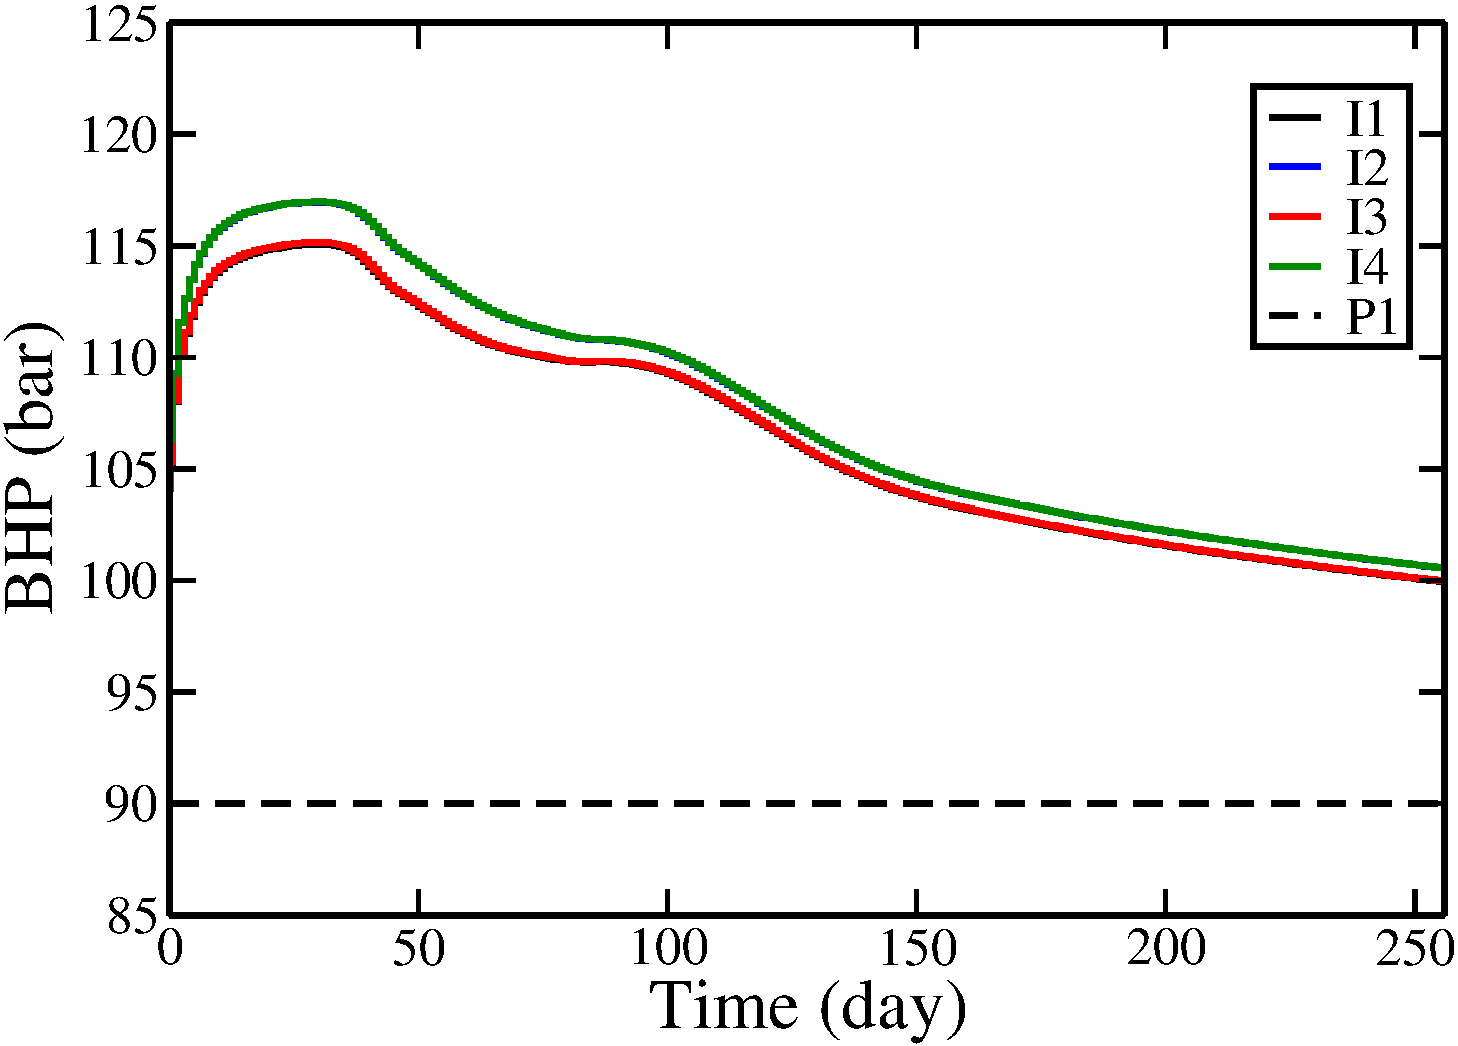
\includegraphics[totalheight=2.2in,angle=0]{figures/ReferenceC500HeuristicItPb_BHP.pdf}
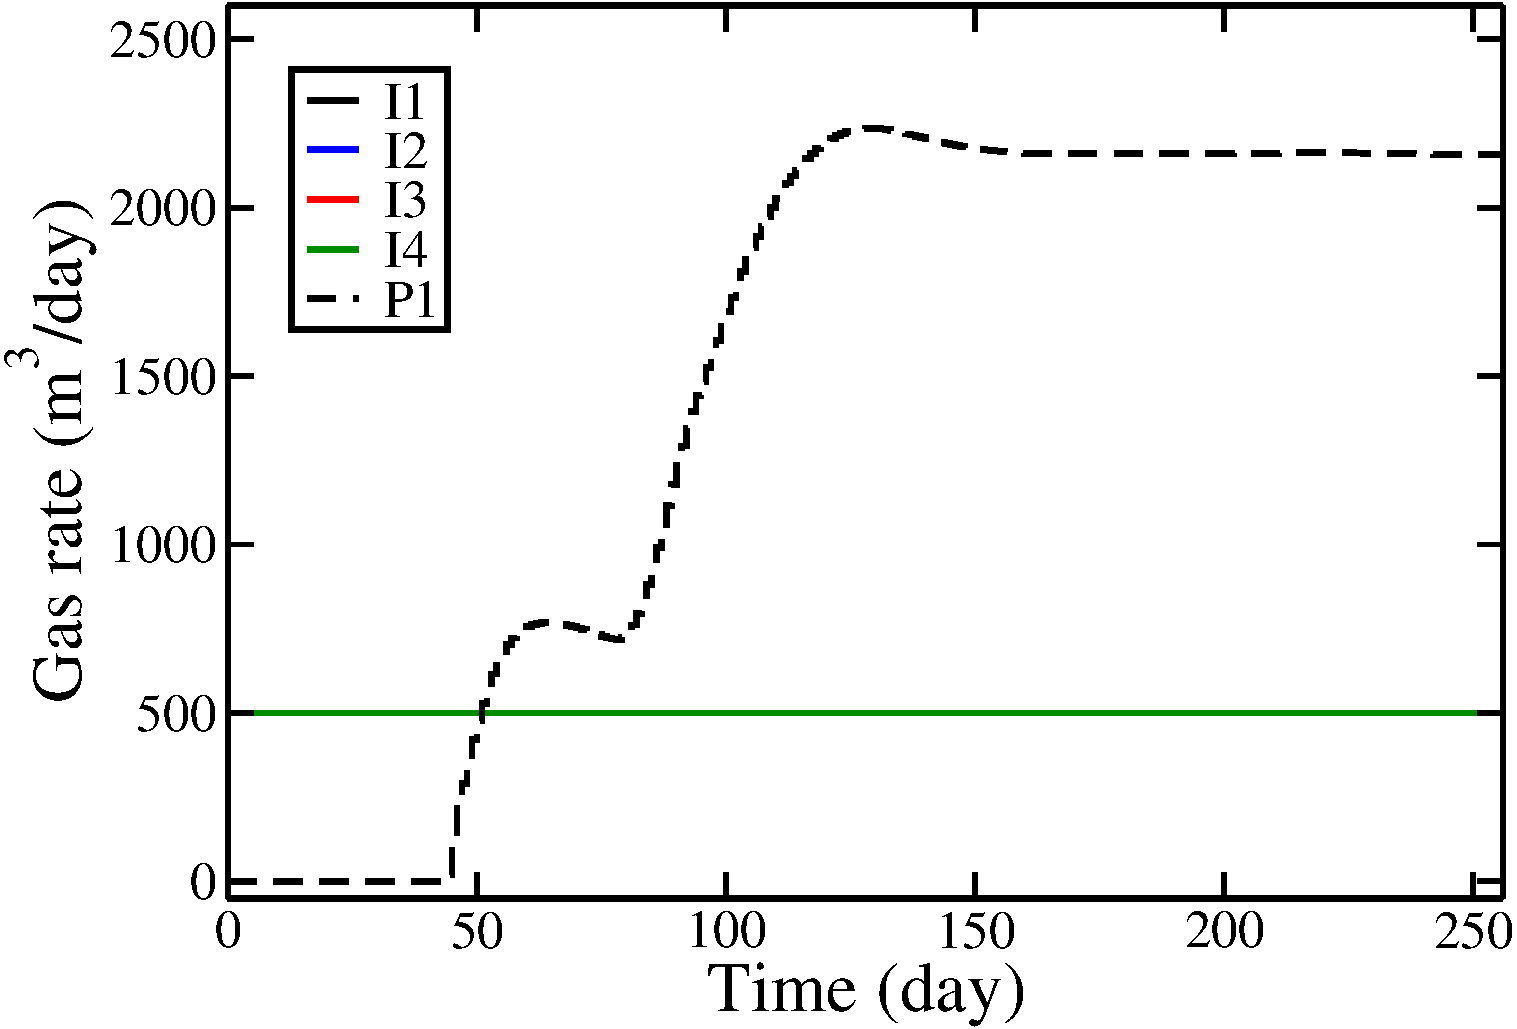
\includegraphics[totalheight=2.17in,angle=0]{figures/ReferenceC500HeuristicItPb_rate_gas.pdf}
\end{center}
\caption{BHPs (top) and gas rates (bottom) for the feasible reference solution (Example 1). 
  Gas injection rates are all equal to 500~m$^3$/d during the entire simulation period. }
\label{fig:PIReferencePlots}
\end{figure}




%%%%%%%%%%%%%%%%%%%%%%%%%%% Pi 40 controls    %%%%%%%%%%%%%%%%%%%%%%%%%%%%%%

\begin{figure}
\begin{center}
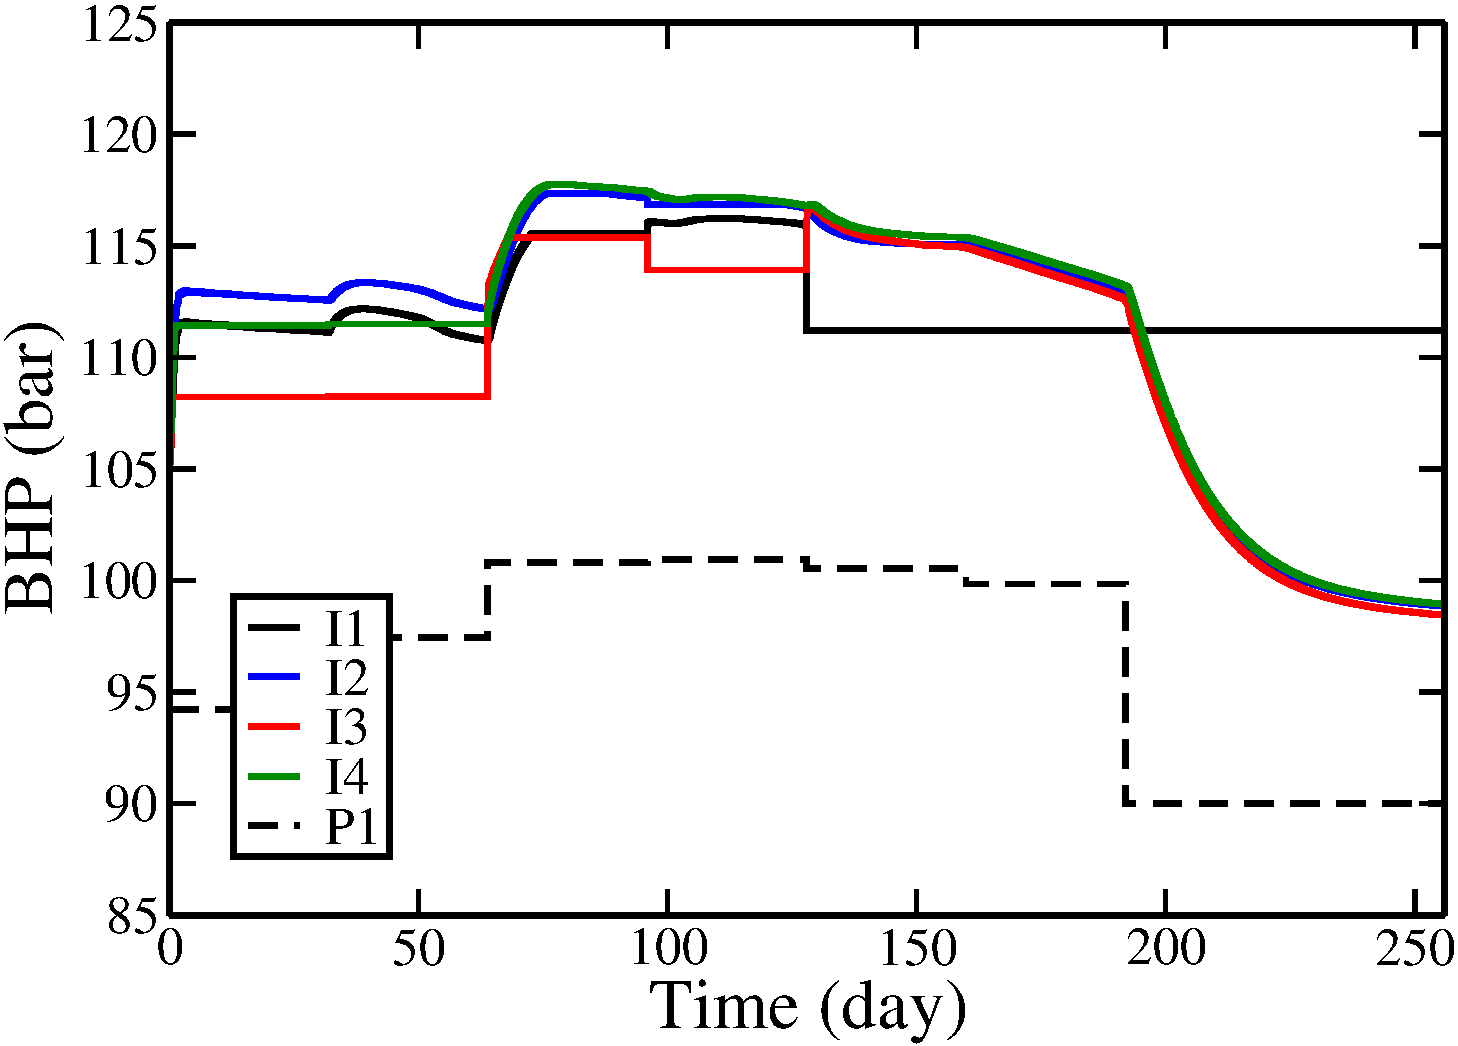
\includegraphics[totalheight=2.2in,angle=0]{figures/HeuristicC500Steps8OptimalItPm_BHP.pdf}
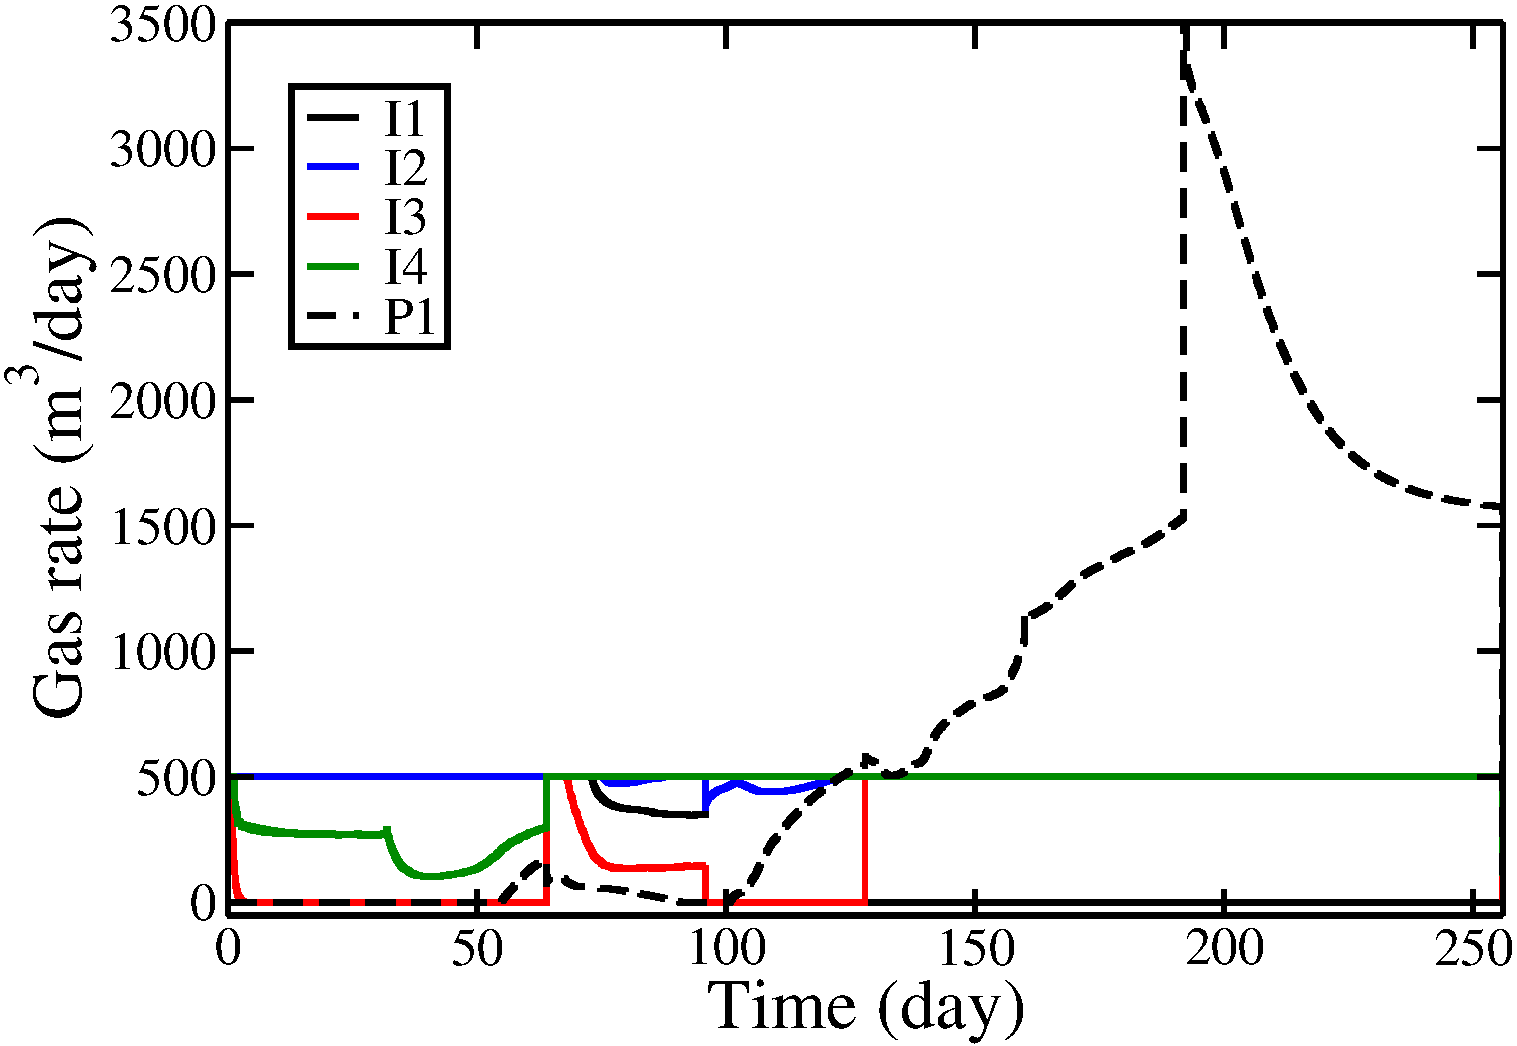
\includegraphics[totalheight=2.17in,angle=0]{figures/HeuristicC500Steps8OptimalItPm_rate_gas.pdf}
\end{center}
\caption{BHPs (top) and gas rates (bottom) for the best heuristically constrained solution using 40 controls (Example 1, Run 8).}
\label{fig:PIHeuristicControls40Plots}
\end{figure}

\begin{figure}
\begin{center}
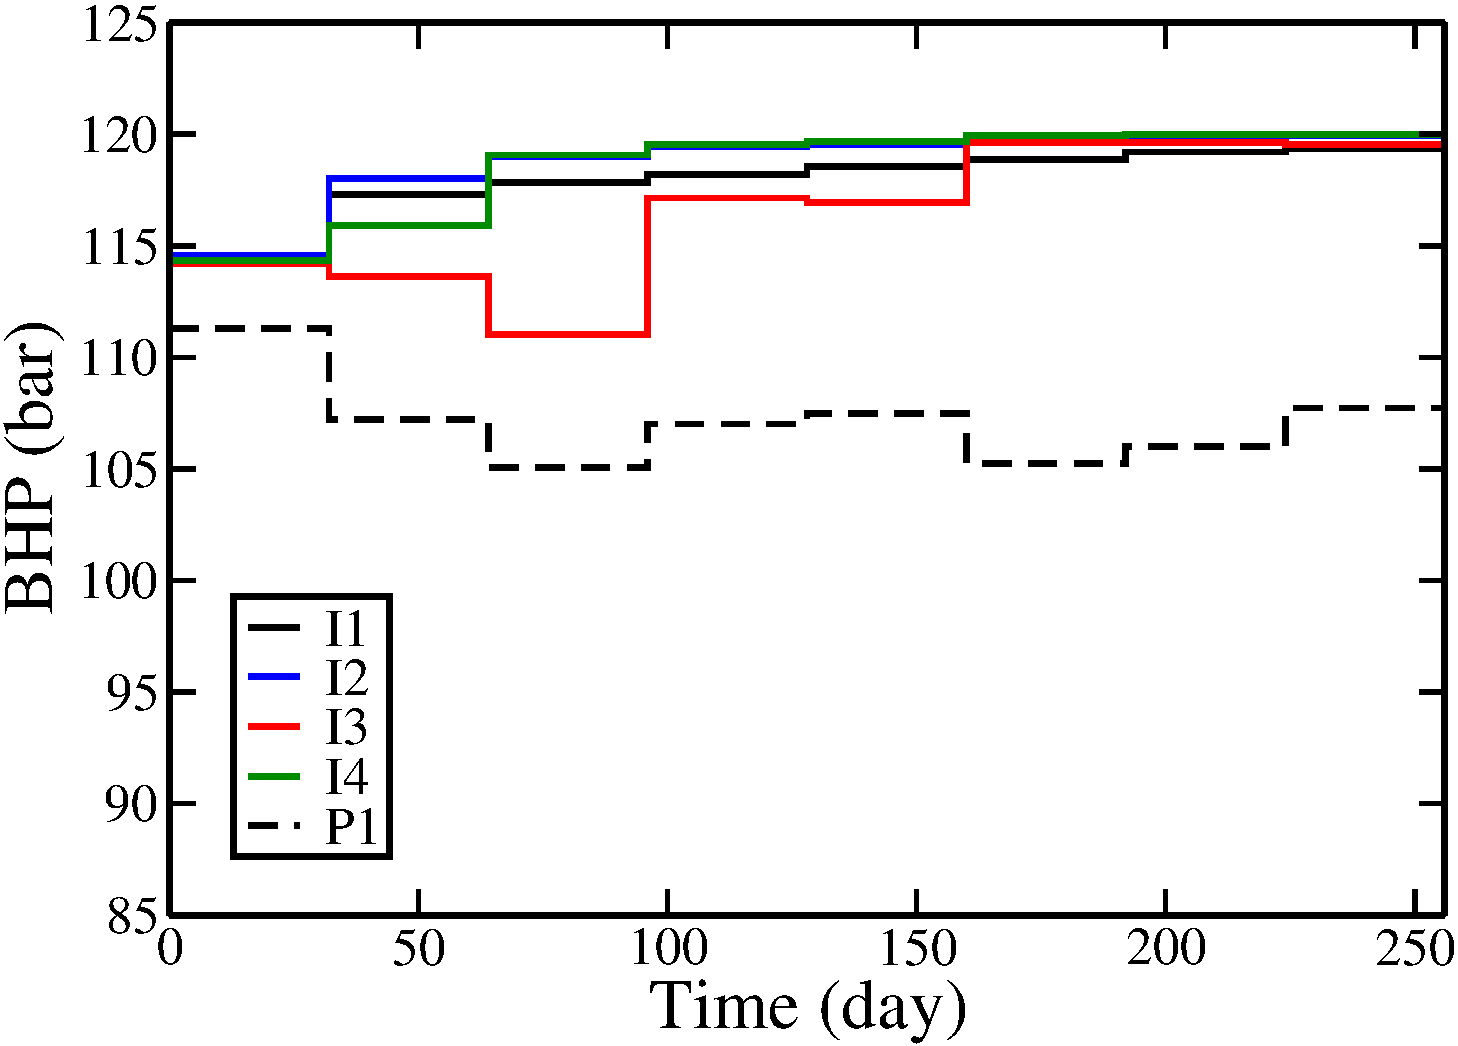
\includegraphics[totalheight=2.2in,angle=0]{figures/FormalC550Steps8OptimalImPb_BHP.pdf}
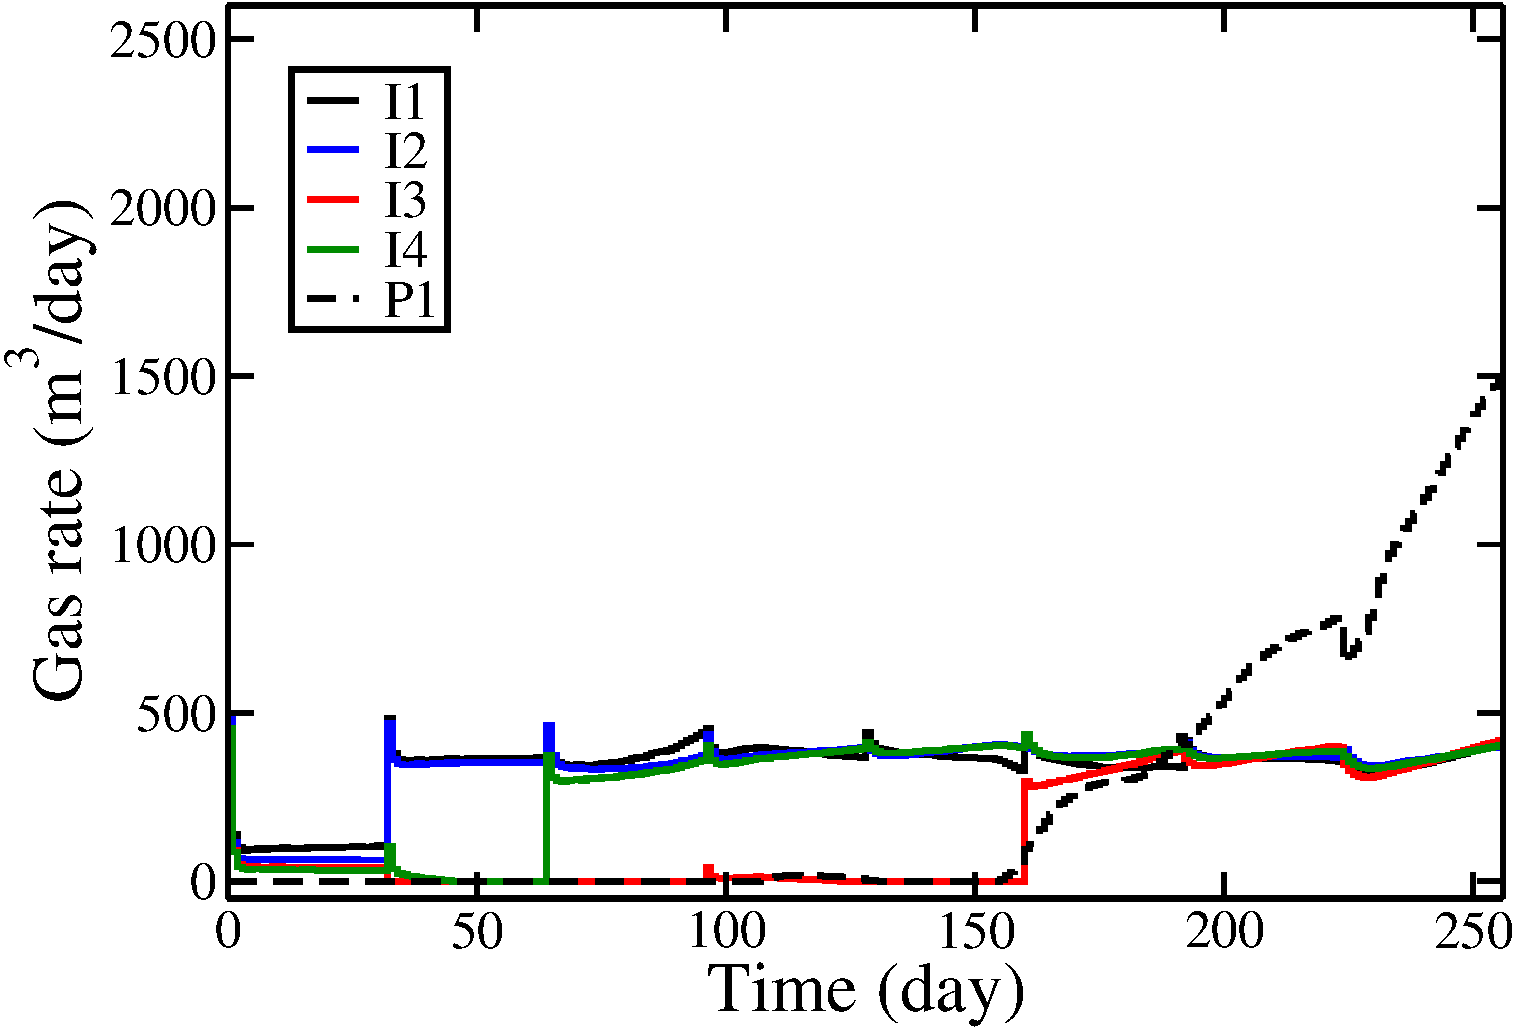
\includegraphics[totalheight=2.17in,angle=0]{figures/FormalC550Steps8OptimalImPb_rate_gas.pdf}
\end{center}
\caption{BHPs (top) and gas rates (bottom) for the best formally constrained solution using 40 controls (Example 1, Run 4).}
\label{fig:PIFormalControls40Plots}
\end{figure}




\begin{figure}
\begin{center}
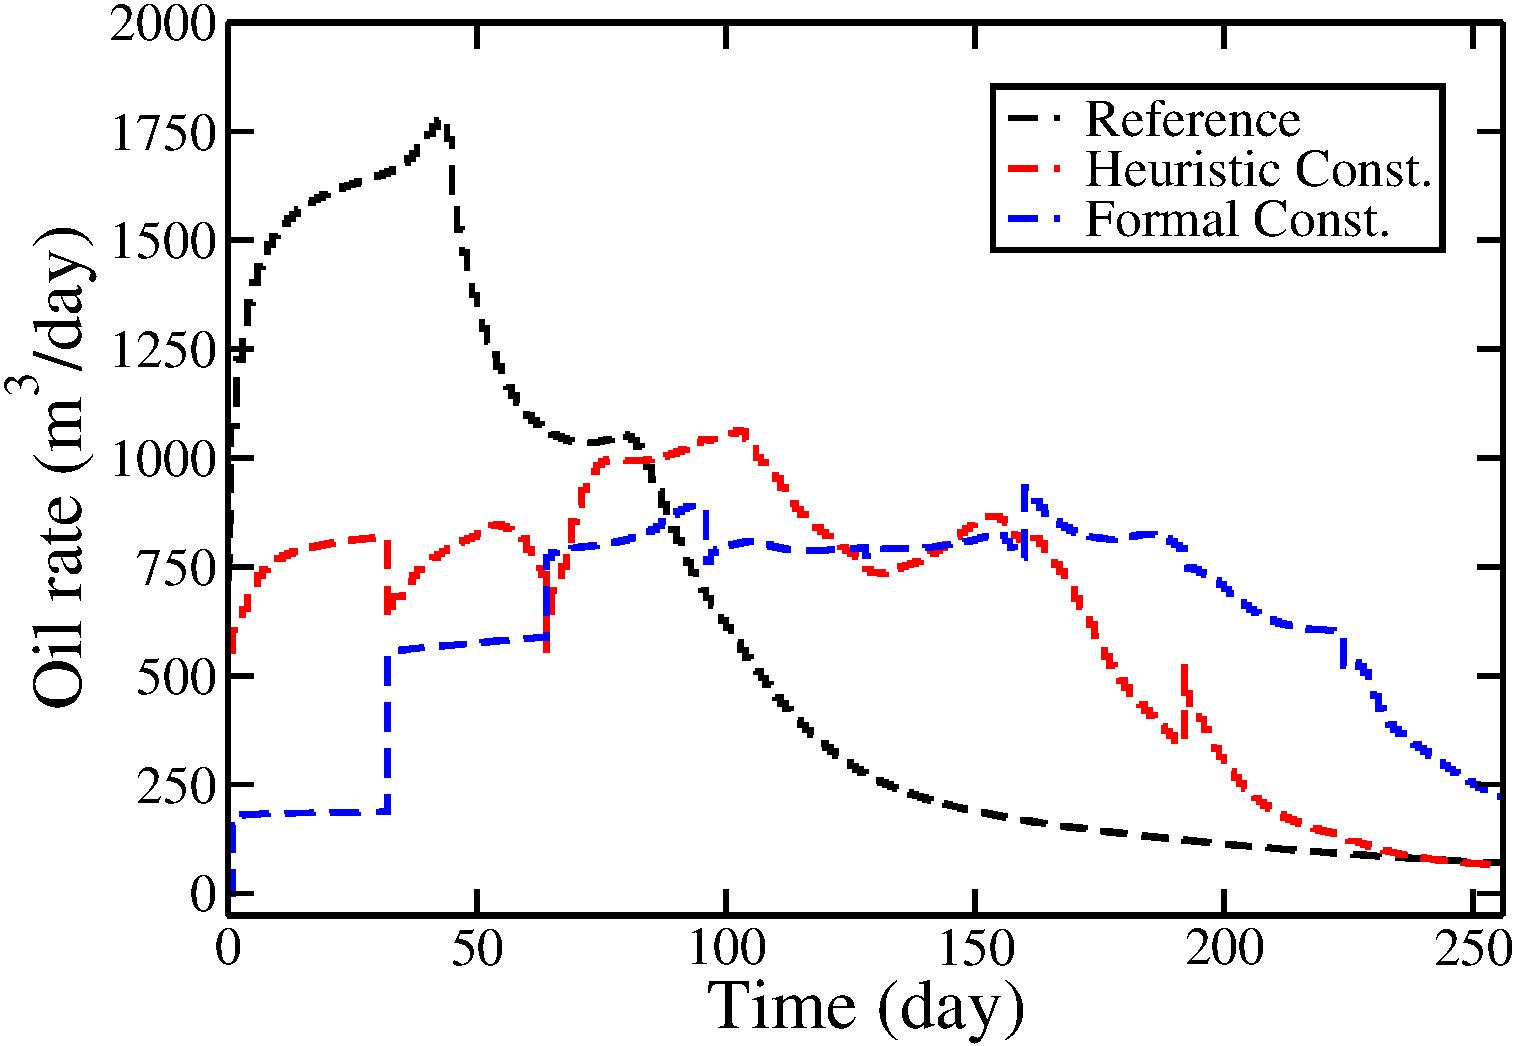
\includegraphics[totalheight=2.2in,angle=0]{figures/OilRatesSteps8.pdf}
%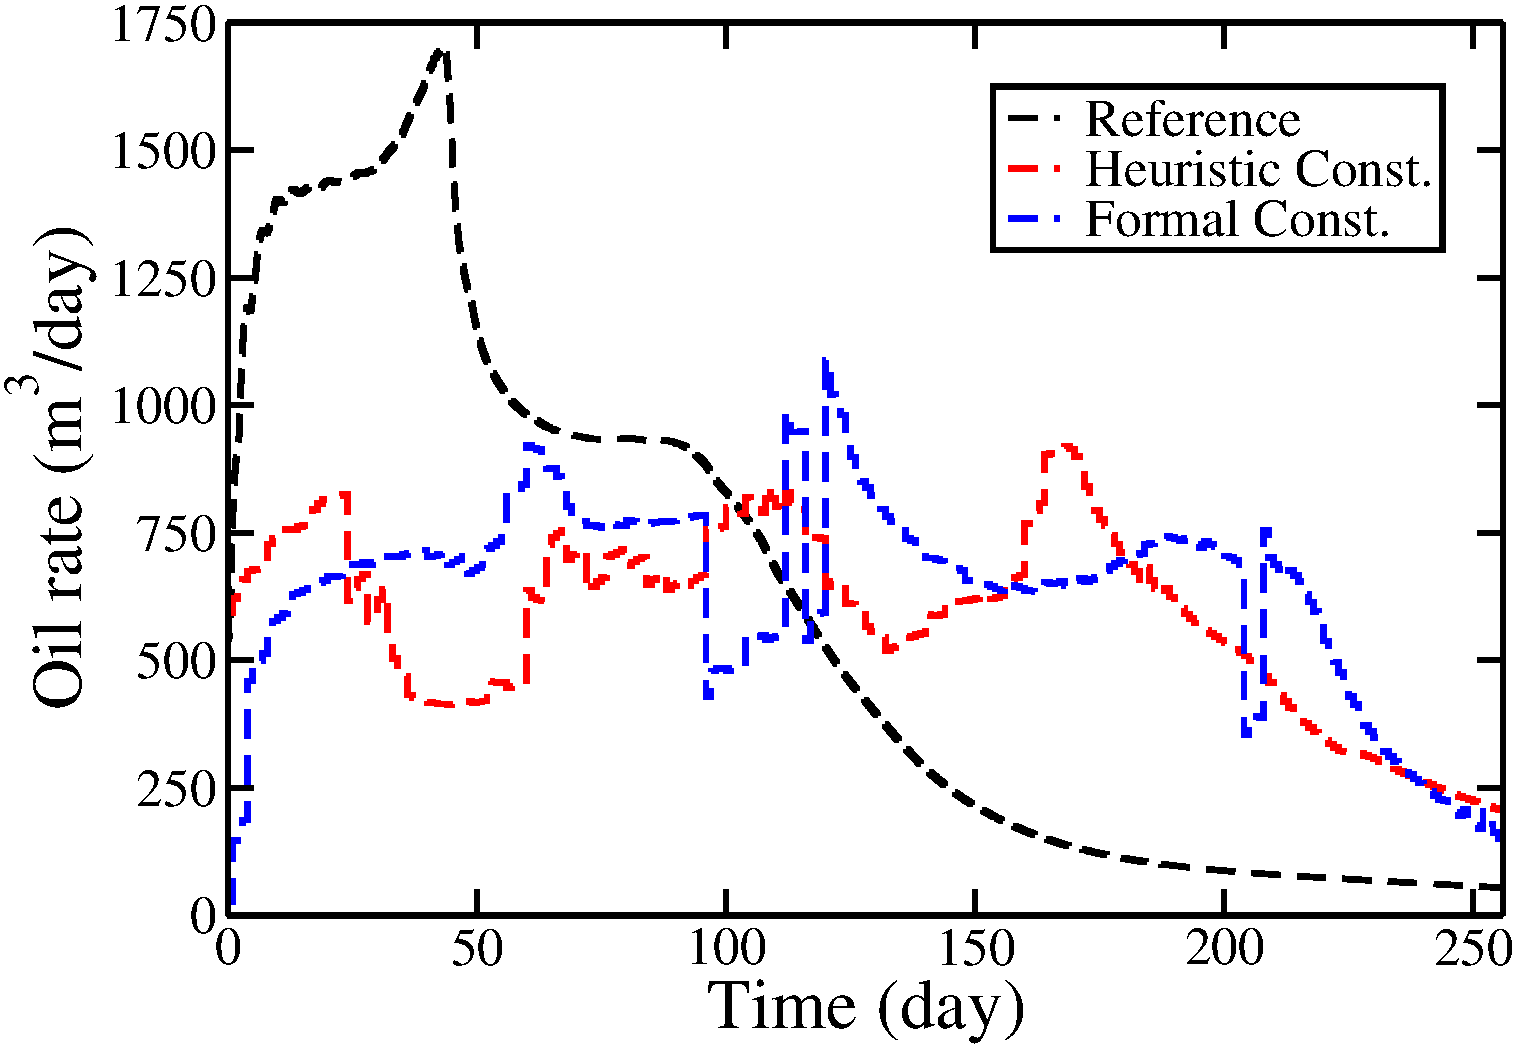
\includegraphics[totalheight=2.2in,angle=0]{OilRatesSteps64.pdf}
%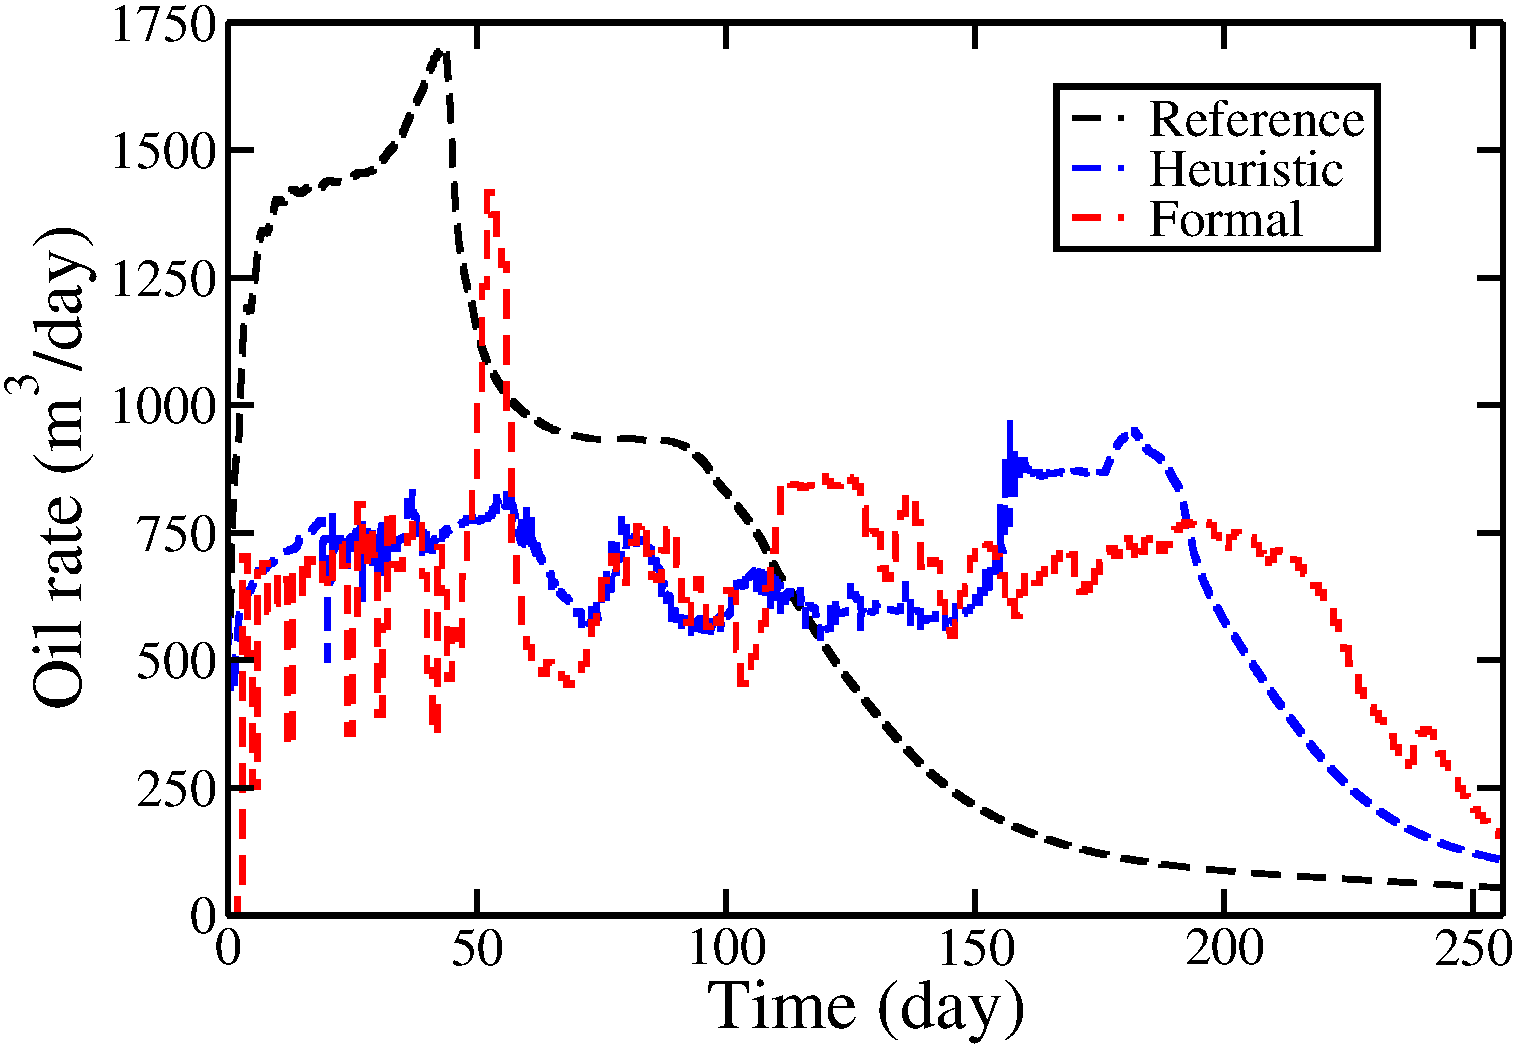
\includegraphics[totalheight=2.2in,angle=0]{OilRates.pdf}
\end{center}
\caption{Oil rates for Example 1 (40 controls), reference (black dashed line), heuristically constrained (red dashed line)
 and formally constrained (blue dashed line).} 
\label{fig:PIOilRates}
\end{figure}





\subsection{Example 2 - Top layer of SPE 10 model}
%
In the second example we again maximize cumulative oil recovery under CO$_2$
injection. The two-dimensional geological model is the top layer of the model
defined in the SPE comparative solution project~\cite{Christie}, referred to as
SPE~10. The model includes a total of four components, as specified in
Table~\ref{table:fluidForSPE10TopLayer}. Details on the
reservoir model are provided in
Table~\ref{table:spe10toplayer}.

%
\begin{table}
\centering
\caption{Fluid description for Example 2}
\begin{tabular}{|l|r|r|r|r|}
\hline
%\multicolumn{5}{|c|}{SPE10 top layer}    \\
%\hline
Component            & CO$_2$ & C$_1$ & C$_4$ & C$_{10}$    \\
\hline
Initial composition (\%)  & 1    & 20  & 29    & 50 \\
Injection composition (\%)& 90   & 10 & - & - \\
\hline
\end{tabular}
\label{table:fluidForSPE10TopLayer}
\end{table}
%


\begin{table}
\centering
\caption{Model parameters for Example 2}
\begin{tabular}{|l|rr|}
\hline
%\multicolumn{3}{|c|}{SPE10 top layer}  \\
%\hline
Grid size                & 60 $\times$ 220 $\times$ 1 &       \\
\hline\hline
Parameter                & Value    & Units \\
\hline
$\Delta x$               & 6.096&m          \\
$\Delta y$               & 3.048&m          \\
$\Delta z$               & 0.6096&m         \\
Depth                    & 2574&m           \\
Initial pressure         & 75  & bar        \\
Temperature              &$100$ & $^\circ$C     \\
\hline
Rock compressibility     & $7.2 \times 10^{-5}$ & 1 / bar \\
Simulation time          &1000 & d          \\
Pressure upper bound     & 150 & bar        \\
Pressure lower bound     &  50 & bar        \\
\hline
Residual gas saturation  & 0 & -            \\
Residual oil saturation  & 0 & -            \\
End point rel perm gas   & 1 & -            \\
End point rel perm oil   & 1 & -            \\
Corey exponent gas       & 2 & -            \\
Corey exponent oil       & 2 & -            \\
\hline\hline
Well locations [grid block no.] & $i$ & $j$     \\
\hline
Injector 1               &   58&   9   \\
Injector 2               &   58& 126   \\
Injector 3               &    2&  67   \\
Injector 4               &    2& 211   \\
Producer 1               &    2&   3   \\
Producer 2               &   58&  67   \\
Producer 3               &    2& 143   \\
Producer 4               &   58& 210   \\
\hline
\end{tabular}
\label{table:spe10toplayer}
\end{table}



The well locations, along with a map of the permeability field, are depicted in
Fig.~\ref{fig:PermeabilityMapAndWellsSpe10Top}. The control parameters in the
optimization problem are again well BHPs, constrained to lie between 150~bar and 50~bar. A
maximum (per well) gas production rate of 200~m$^3/$d at reservoir conditions is also specified.
The total simulation period is 1000~days. The well controls are determined
at initial time and then at every 100-day interval. There are a
total of ten control steps and 80 control parameters in this example.


%
\begin{figure}[ht]
\begin{center}
     \begin{tabular}{cccccccc}
      0.003 &  0.023 & 0.178 & 1.358 & 10.38 & 79.43 & 607.6 &4648
      \end{tabular}
      \includegraphics[width=8cm, height=0.5cm]{figures/VanEssenModelPermeabilityMapColorBar.png}
       
       \medskip

       \includegraphics[totalheight=3.2in]{figures/SPE10TopModelPermeabilityMapConstantRotated.png} %SPE10TopPermeabilityMapAndWells.png}

        %\medskip

       %\includegraphics[totalheight=3.2in, angle=270]{SPE10TopModelPermeabilityMapConstant.png} %SPE10TopPermeabilityMapAndWells.png}
\end{center}
     \caption{Injection wells (blue) and production wells (red) for Example~2. Background shows $\log \tens{k}_x$ ($\tens{k}_x = \tens{k}_y$).}
  \label{fig:PermeabilityMapAndWellsSpe10Top}
\end{figure}
%

\begin{table}
\centering
\caption{Oil production in $10^3$~m$^3$ (Example 2) for the optimized objective function
         without satisfying the nonlinear constraints (`Unconstr.'), satisfying the nonlinear constraints
         using the heuristic treatment (`Heuristic'), and satisfying the nonlinear constraints
         using the formal approach (`Formal'). Best feasible results shown in bold.}
\begin{tabular}{|c|c|c|c|}
\hline
  Run            &  Unconstr. & Heuristic & Formal      \\
\hline
Reference        & 20.29         &     20.28         & 	         \\
1 & 21.77      &     21.77         &       21.77    \\
2 & 22.01      &     22.01         &       22.01    \\
3 & 18.16      &     18.16         &       18.17    \\
4 & 21.68      &     21.68         &       21.68    \\
5 & 22.03      & \bf{22.03}      &       22.04    \\
6 & 22.13      &     20.67         &  \bf{22.20}    \\
7 & 21.68      &     21.68         &       21.99    \\
8 & 22.07      &     21.48         &       22.07    \\
9 & 22.03      & \bf{22.03}      &       22.03    \\
\hline
\end{tabular}
  \label{table:spe10top}
\end{table}

%1 & O25G16     &     21400         &       O78G57 \\
%2 & O25G16     & \bf{21980}        &       O46G35 \\
%3 & O48G34     &     16800         &       O31G22 \\
%4 & O25G17     &     21600         &       O79G46 \\
%5 & O21G17     &     19900         &       O140G62\\
%6 & O28G15     &     19800         &       O41G32 \\
%7 & O24G15     &     21000         &       O77G61 \\
%8 & O21G14     &     20500         &       O67G49 \\
%9 & O29G19     &     20900         &       O77G49 \\


We first generate two reference solutions as in the previous example. The cumulative oil production for these two cases, given in the first row (`Reference') of Table~\ref{table:spe10top}, are nearly identical because the nonlinear constraint violation in the
unconstrained case is small. We next perform (nine) optimizations that honor the bound constraints but not the nonlinear constraints. The best optimum achieved in this case provides a cumulative oil production of 22,130~m$^3$ (Run~6). Using the heuristic constraint handling procedure (third column), the best result is 22,030~m$^3$ of oil (Runs~5 and 9), which
exceeds the reference heuristic result by 8.8\%. The best optimum achieved using the formal constraint handling treatment is 22,200~m$^3$ of oil (Run~6). This value exceeds the reference solution by 9.5\% and the best result using the heuristic treatment by 0.8\%. It also exceeds the best unconstrained result (again, unconstrained here refers to the nonlinear constraints) of 22,130~m$^3$, which is presumably because the nonlinear constraints are not very important in this example.

Oil production profiles are shown in Fig.~\ref{fig:SPE10TopLayerRevenue}. These profiles are very similar for the runs using the heuristic and formal constraint handling procedures. The BHP, gas rate, and oil rate profiles for the three cases are shown in
Figs.~\ref{fig:SPE10TopLayerReferenceRates},
\ref{fig:SPE10TopLayerUnconstrainedOptimalChoppedRates} and
\ref{fig:SPE10TopLayerConstrainedOptimalRates}. We see that the gas production rates satisfy the nonlinear constraints (200~m$^3/$d) at all times for both constraint handling procedures. Consistent with Fig.~\ref{fig:SPE10TopLayerRevenue}, the oil production rates in Figs.~\ref{fig:SPE10TopLayerUnconstrainedOptimalChoppedRates} and
\ref{fig:SPE10TopLayerConstrainedOptimalRates} resemble one another, and they are clearly different than the reference solution in Fig.~\ref{fig:SPE10TopLayerReferenceRates}. 
For this example, the formal approach required an average of 56 forward simulations, while the heuristic approach required an average of only 24.


\begin{figure} [ht]
\begin{center}
\includegraphics[totalheight=2.17in,angle=0]{figures/spe10TopLayerRevenue.pdf}
\end{center}
\caption{Oil production versus time for Example 2. Results are for
  feasible reference case (black curve), best heuristically constrained solution (Run~9, red curve)
  and best formally constrained solution (Run~6, blue curve).}
\label{fig:SPE10TopLayerRevenue}
\end{figure}
\begin{figure}
\begin{center}
\includegraphics[totalheight=2.2in,angle=0]{figures/spe10topLayerReferenceC200_BHP.pdf}
\includegraphics[totalheight=2.17in,angle=0]{figures/spe10topLayerReferenceC200_rate_gas.pdf}
\includegraphics[totalheight=2.2in,angle=0]{figures/spe10topLayerReferenceC200_rate_oil.pdf}
\end{center}
\caption{BHPs (top), gas rates (middle) and oil rates
  (bottom) for the feasible reference solution (Example 2).}
\label{fig:SPE10TopLayerReferenceRates}
\end{figure}

\begin{figure}
\begin{center}
\includegraphics[totalheight=2.2in,angle=0]{figures/spe10topLayerOptimalChoppedIuPu_BHP.pdf}
\includegraphics[totalheight=2.17in,angle=0]{figures/spe10topLayerOptimalChoppedIuPu_rate_gas.pdf}
\includegraphics[totalheight=2.2in,angle=0]{figures/spe10topLayerOptimalChoppedIuPu_rate_oil.pdf}
\end{center}
\caption{BHPs (top), gas rates (middle) and oil rates
  (bottom) for the best heuristically constrained solution (Example 2, Run 9).}
\label{fig:SPE10TopLayerUnconstrainedOptimalChoppedRates}
\end{figure}
\begin{figure}
\begin{center}
\includegraphics[totalheight=2.2in,angle=0]{figures/spe10TopLayerConstrainedOptimalIuPa_BHP.pdf}
\includegraphics[totalheight=2.2in,angle=0]{figures/spe10TopLayerConstrainedOptimalIuPa_rate_gas.pdf}
\includegraphics[totalheight=2.2in,angle=0]{figures/spe10TopLayerConstrainedOptimalIuPa_rate_oil.pdf}
\end{center}
\caption{BHPs (top), gas rates (middle) and oil rates
  (bottom) for the best formally constrained solution (Example 2, Run 6).}
\label{fig:SPE10TopLayerConstrainedOptimalRates}
\end{figure}



\subsection{Example 3: Twelve-well channelized system}


Our third example uses the three-dimensional geological model introduced in
\cite{VanEssen}. We again consider CO$_2$ injection, though this model
contains a total of six components, defined in
Table~\ref{table:VanEssenModelFluid}. Further details are given in Table~\ref{table:VanEssenModelReservoir}.  A map of
the $x$-component of permeability (here $\tens{k}_x = \tens{k}_y = 10\tens{k}_z$), along with the
locations of the wells, is shown in Fig.~\ref{fig:VanEssenModelPermeabilityAndWells}.


\begin{figure}[ht]
     \begin{center}
      \begin{tabular}{cccccccc}
      53.90 & 108.0 & 216.5 & 433.9 & 569.6 & 1743 & 3493 & 7000 
      \end{tabular}
       \includegraphics[width=8cm,height=0.5cm]{figures/VanEssenModelPermeabilityMapColorBar.png}
                                                            
       \medskip
       
       \includegraphics[width=8cm]{figures/VanEssenModelPermeabilityMapConstant.png}%VanEssenModelPermeabilityMap.png}
%       \includegraphics[totalheight=10.5cm]{pdf/VanEssenModelPermeabilityXLogTransparent.pdf}
     \end{center}
     \caption{Reservoir model and wells for Example 3 (from \cite{VanEssen}). Background shows $\log \tens{k}_x$.}
  \label{fig:VanEssenModelPermeabilityAndWells}
\end{figure}



\begin{table}
\tabcolsep=0pt
\centering
\caption{Fluid description for example 2}
\begin{tabular*}{84mm}{@{\extracolsep\fill}lllllll}\toprule
Component            & CO$_2$ & C$_1$ & C$_2$ & C$_3$ & C$_4$  & C$_{10}$ \\[2pt]
\midrule
Initial comp. (\%)   & 1    & 20  & 30  & 19  & 10   & 20     \\
Injection comp. (\%) & 95   &  1  &  1  &  1  &  1   &  1     \\
\bottomrule
\end{tabular*}
\label{table:VanEssenModelFluid}
\end{table}


\begin{table}
\tabcolsep=0pt
\centering
\caption{Model parameters for example 2.}
\label{table:VanEssenModelReservoir}
\begin{tabular*}{84mm}{@{\extracolsep\fill}lll}\toprule
Parameter                      & Value           & Units     \\
\midrule
Grid size                      & 60 $\times$ 60 $\times$ 7 &  ---      \\
$\Delta x$                     & 24           & m            \\
$\Delta y$                     & 24           & m            \\
$\Delta z$                     &  4           & m            \\
Depth                          & 2538       & m              \\
Initial pressure               & 100          & bar          \\
Temperature                    & $372$     & $^\circ$C       \\
Rock compressibility           & $10^{-5}$    & 1 / bar      \\
Simulation time                & 300          & d            \\
Pressure upper bound           & 120          & bar          \\
Pressure lower bound           &  90          & bar          \\
Residual gas saturation  & 0 & ---                           \\
Residual oil saturation  & 0 & ---                           \\
End point rel perm gas   & 1 & ---                           \\
End point rel perm oil   & 1 & ---                           \\
Corey exponent gas       & 2 & ---                           \\
Corey exponent oil       & 2 & ---                           \\[2pt]
\bottomrule
Well locations [grid block no.] & $i$ & $j$                  \\
\midrule
Injector 1               &  5 &  57                          \\
Injector 2               &  30&  53                          \\
Injector 3               &   2&  35                          \\
Injector 4               &  27&  29                          \\
Injector 5               &  50&  35                          \\
Injector 6               &   8&   9                          \\
Injector 7               &  32&   2                          \\
Injector 8               &  57&   6                          \\
Producer 1               &  16&  43                          \\
Producer 2               &  35&  40                          \\
Producer 3               &  23&  16                          \\
Producer 4               &  43&  18                          \\[2pt]
\bottomrule
\end{tabular*}
\end{table}





The control parameters of our optimization problem are again the well BHPs.  The
wells are constrained to operate between an upper bound of 120~bar and a lower
bound of 90~bar. We also specify nonlinear constraints on both injection and
production in the form of maximum gas flow
rates of 200,000~m$^3/$d for the producers and 40,000~m$^3/$d for the injectors
(both at reservoir conditions). This model is run for a total of 100 days, and
we control the BHPs at initial time and then every ten days (the simulation time
frame is short in this case because the problem specification is such that oil
is produced quickly). There are a total of 120 control parameters in this
problem, and our objective is again to maximize cumulative oil production.

We simulate this model using the same procedures as in the previous examples.
Results for the nine runs for each case are presented in
Table~\ref{table:vanessen}. The feasible reference case yields 5.030$\times 10^6$~m$^3$ of
oil, while the best heuristically constrained case (Run~2) provides 5.457$\times 10^6$~m$^3$
of oil, an improvement of 8.5\%. The best formally constrained case (Run~3)
achieves an optimum of 5.306$\times 10^6$~m$^3$ of oil, which exceeds the reference case by
5.5\% but is less than the best heuristic case. The oil production profiles
for the best runs, along with the feasible reference case, are shown in
Fig.~\ref{fig:VanEssenRevenue}. We again see that the early time production in
the reference case exceeds that of the optimized cases, though the cumulative
oil produced in the optimized cases is of course higher. 

In this example, convergence of the optimizations using the formal constraint handling approach 
typically required about 48 forward simulations, while the heuristic treatment required only about 26. Our findings for this example clearly illustrate the potential advantages of the heuristic treatment for complex optimization problems involving multiple wells operating under nonlinear constraints.



\begin{table}
\centering
\caption{Oil production in $10^6$~m$^3$ (Example 3) for the optimized objective function
         without satisfying the nonlinear constraints (`Unconstr.'), satisfying the nonlinear constraints
         using the heuristic treatment (`Heuristic'), and satisfying the nonlinear constraints
         using the formal approach (`Formal'). Best feasible results shown in bold.}
\begin{tabular}{|c|c|c|c|}
\hline
 Run              & Unconstr. & Heuristic & Formal     \\
\hline
Reference         & 5.030 &  5.030    &          \\
1 & 5.450 &  5.449   &  5.284   \\
2 & 5.467 &\bf{5.457} &  5.294   \\
3 & 5.171 &  5.171   &\bf{5.306}\\
4 & 5.288 &  5.287   &  5.132   \\
5 & 5.424 &  5.423   &  5.224   \\
6 & 5.344 &  5.348   &  5.260   \\
7 & 5.321 &  5.230   &  4.994   \\
8 & 5.207 &  5.205   &  5.196   \\
9 & 5.353 &  5.349   &  4.986   \\
\hline
\end{tabular}
  \label{table:vanessen}
\end{table}


%1 & O30G23 5.450    &  5.2976    &  O41G30 5.284         \\
%2 & O47G27 5.467    &\bf{5.46} &  O46G30 5.294         \\
%3 & O22G12 5.171    &  5.02    &  O44G30 \bf{5.306}    \\
%4 & O25G18 5.288    &  5.02    &  O28G13 5.132         \\
%5 & O43G27 5.424    &  5.29    &  O35G30 5.224         \\
%6 & O43G19 5.344    &  5.35    &  O48G38 5.260         \\
%7 & O31G18 5.321    &  5.20    &  O43G29 4.994         \\
%8 & O19G10 5.207    &  5.21    &  O37G25 5.196         \\
%9 & O13G10 5.353    &  5.19    &  O91G26 4.986         \\


\begin{figure} [ht]
\begin{center}
\includegraphics[totalheight=2.2in,angle=0]{figures/vanEssenRevenue.pdf}
\end{center}
\caption{Oil production versus time for Example 3. Results are for
  feasible reference case (black curve), best heuristically constrained solution (Run 2, red curve)
  and best formally constrained solution (Run 3, blue curve).}
\label{fig:VanEssenRevenue}
\end{figure}



\section{Concluding remarks}  \label{sec:conclusions}
In this work we formulated and tested an adjoint-based optimization procedure
for compositional reservoir simulation. The method we employed was implemented into
Stanford's Automatic Differentiation-based General Purpose Research Simulator
(AD-GPRS). The use of automatic differentiation simplifies the adjoint
implementation and subsequent code enhancements. Two different treatments for
handling nonlinear constraints were presented. In the formal constraint handling
procedure, lumped constraints and their gradients are provided to the optimizer,
and feasibility is enforced by the optimization algorithm. In the second
(heuristic) procedure, an optimization satisfying only the bound and linear
constraints is performed first. Then, the forward model is run using the
controls from the first stage, but the simulator is allowed to switch from BHP
to rate control (for a problem in which BHPs are the control variables) as
required to satisfy the nonlinear rate constraints.


Numerical results were presented for four example cases of increasing
complexity. Nine runs, starting from different initial conditions, were
performed in all cases, for both the heuristic and the formal nonlinear
constraint treatments. In our examples, the control variables were the time-varying well BHPs, and maximum injection or production rate specifications entered as nonlinear
constraints. The total number of control variables ranged from 40 to 320. Improvement in cumulative oil produced (which was the objective function in all cases) using our optimization procedures ranged from 4.2\% to 11.6\% relative to the reference solutions. 

In the simplest case (Example~1), the formal constraint handling approach was shown to outperform the heuristic procedure when we increased the number of control variables from 40 to 320. In the next (somewhat more complicated) case, Example~2, the formal constraint treatment continued to outperform the heuristic procedure, though its advantage was very slight. In the other two cases, which were more challenging in terms of model size and number of wells (and they involved three-dimensional models, while the first two examples were two-dimensional), the heuristic treatment provided better objective function values than the formal approach. 

These observations suggest that, although the formal constraint handling approach is theoretically superior, complications related to constraint lumping and the existence of poor local optima (and the additional complexity inherent in problems with large numbers of optimization variables and nonlinear constraints) may render the formal procedure less effective than the heuristic approach in challenging cases. Thus, though we expect (and observe) the formal procedure to be the method of choice in relatively simple cases, the heuristic approach should be considered for use in more complex problems. It may even be beneficial to apply some type of hybrid technique, where the result from the heuristic method is used as the initial guess for the formal procedure. The use of a sequence of optimizations, with increasing numbers of control periods, should also be considered. Finally, it is important to note that the heuristic constraint treatment was found to be significantly more efficient than the formal approach. 


In addition to the discrete adjoint procedure, which was used for all of the
examples presented in this paper, we also derived and implemented a continuous
adjoint formulation. We showed that the two formulations use different
final time conditions and as a result the gradients do not
agree in general. However, the two boundary conditions become almost identical as the
size of the last time step approaches zero, in which case the gradients obtained by
both formulations are essentially the same.

There are a number of areas in which future research should be directed. Other
treatments for nonlinear constraints, both formal and heuristic, should be
considered, and the relative benefits of controlling rates instead of BHPs
should be assessed. It will be of interest to apply the general optimization
framework to larger and more realistic simulation models. Other types of wells
(horizontal, deviated, multilateral) should also be considered, along with the
optimization of downhole inflow control devices. The overall approach can be 
extended to perform robust control (to account for geological uncertainty) and hierarchical
(multi-objective) control to balance long-term and short-term objectives. Finally, our procedures could be applied for the optimization of CO$_2$ storage or for combined
EOR-CO$_2$ storage operations.



\section*{Acknowledgements}
We thank Denis Voskov and Oleg Volkov for useful discussions and assistance with AD-GPRS, and
Michael Saunders for his support 
on SNOPT. We are grateful
to the industrial affiliates of the Stanford University Smart Fields Consortium for partial
funding of this work.






\part{Numerical examples}
%%%%%%%%%%%%%%%% Apendices  %%%%%%%%%%%%%%%%%%
\appendix
\include{appendix1}
\include{appendix2}
\include{appendix3}
%%%%%%%%%%%%%%%%%%%%%%%%%%%%%%%%%%%%%%%%%%%%%%

%%%%%%%%%%% Back matter starts %%%%%%%%%%%%%%%
\backmatter
%%%%%%%%%%%%%%%%%%%%%%%%%%%%%%%%%%%%%%%%%%%%%%

\printindex

\clearpage

\addcontentsline{toc}{chapter}{Bibliography}
\bibliographystyle{apalike}      % mathematics and physical sciences
\bibliography{ptyxiakh}



\end{document}
%%% Local Variables: 
%%% mode: latex
%%% TeX-master: t
%%% End: 
